\documentclass[]{book}
\usepackage{lmodern}
\usepackage{amssymb,amsmath}
\usepackage{ifxetex,ifluatex}
\usepackage{fixltx2e} % provides \textsubscript
\ifnum 0\ifxetex 1\fi\ifluatex 1\fi=0 % if pdftex
  \usepackage[T1]{fontenc}
  \usepackage[utf8]{inputenc}
\else % if luatex or xelatex
  \ifxetex
    \usepackage{mathspec}
  \else
    \usepackage{fontspec}
  \fi
  \defaultfontfeatures{Ligatures=TeX,Scale=MatchLowercase}
\fi
% use upquote if available, for straight quotes in verbatim environments
\IfFileExists{upquote.sty}{\usepackage{upquote}}{}
% use microtype if available
\IfFileExists{microtype.sty}{%
\usepackage[]{microtype}
\UseMicrotypeSet[protrusion]{basicmath} % disable protrusion for tt fonts
}{}
\PassOptionsToPackage{hyphens}{url} % url is loaded by hyperref
\usepackage[unicode=true]{hyperref}
\hypersetup{
            pdftitle={R for everyone},
            pdfauthor={Matthew Gemmell},
            pdfborder={0 0 0},
            breaklinks=true}
\urlstyle{same}  % don't use monospace font for urls
\usepackage{natbib}
\bibliographystyle{apalike}
\usepackage{color}
\usepackage{fancyvrb}
\newcommand{\VerbBar}{|}
\newcommand{\VERB}{\Verb[commandchars=\\\{\}]}
\DefineVerbatimEnvironment{Highlighting}{Verbatim}{commandchars=\\\{\}}
% Add ',fontsize=\small' for more characters per line
\usepackage{framed}
\definecolor{shadecolor}{RGB}{248,248,248}
\newenvironment{Shaded}{\begin{snugshade}}{\end{snugshade}}
\newcommand{\KeywordTok}[1]{\textcolor[rgb]{0.13,0.29,0.53}{\textbf{#1}}}
\newcommand{\DataTypeTok}[1]{\textcolor[rgb]{0.13,0.29,0.53}{#1}}
\newcommand{\DecValTok}[1]{\textcolor[rgb]{0.00,0.00,0.81}{#1}}
\newcommand{\BaseNTok}[1]{\textcolor[rgb]{0.00,0.00,0.81}{#1}}
\newcommand{\FloatTok}[1]{\textcolor[rgb]{0.00,0.00,0.81}{#1}}
\newcommand{\ConstantTok}[1]{\textcolor[rgb]{0.00,0.00,0.00}{#1}}
\newcommand{\CharTok}[1]{\textcolor[rgb]{0.31,0.60,0.02}{#1}}
\newcommand{\SpecialCharTok}[1]{\textcolor[rgb]{0.00,0.00,0.00}{#1}}
\newcommand{\StringTok}[1]{\textcolor[rgb]{0.31,0.60,0.02}{#1}}
\newcommand{\VerbatimStringTok}[1]{\textcolor[rgb]{0.31,0.60,0.02}{#1}}
\newcommand{\SpecialStringTok}[1]{\textcolor[rgb]{0.31,0.60,0.02}{#1}}
\newcommand{\ImportTok}[1]{#1}
\newcommand{\CommentTok}[1]{\textcolor[rgb]{0.56,0.35,0.01}{\textit{#1}}}
\newcommand{\DocumentationTok}[1]{\textcolor[rgb]{0.56,0.35,0.01}{\textbf{\textit{#1}}}}
\newcommand{\AnnotationTok}[1]{\textcolor[rgb]{0.56,0.35,0.01}{\textbf{\textit{#1}}}}
\newcommand{\CommentVarTok}[1]{\textcolor[rgb]{0.56,0.35,0.01}{\textbf{\textit{#1}}}}
\newcommand{\OtherTok}[1]{\textcolor[rgb]{0.56,0.35,0.01}{#1}}
\newcommand{\FunctionTok}[1]{\textcolor[rgb]{0.00,0.00,0.00}{#1}}
\newcommand{\VariableTok}[1]{\textcolor[rgb]{0.00,0.00,0.00}{#1}}
\newcommand{\ControlFlowTok}[1]{\textcolor[rgb]{0.13,0.29,0.53}{\textbf{#1}}}
\newcommand{\OperatorTok}[1]{\textcolor[rgb]{0.81,0.36,0.00}{\textbf{#1}}}
\newcommand{\BuiltInTok}[1]{#1}
\newcommand{\ExtensionTok}[1]{#1}
\newcommand{\PreprocessorTok}[1]{\textcolor[rgb]{0.56,0.35,0.01}{\textit{#1}}}
\newcommand{\AttributeTok}[1]{\textcolor[rgb]{0.77,0.63,0.00}{#1}}
\newcommand{\RegionMarkerTok}[1]{#1}
\newcommand{\InformationTok}[1]{\textcolor[rgb]{0.56,0.35,0.01}{\textbf{\textit{#1}}}}
\newcommand{\WarningTok}[1]{\textcolor[rgb]{0.56,0.35,0.01}{\textbf{\textit{#1}}}}
\newcommand{\AlertTok}[1]{\textcolor[rgb]{0.94,0.16,0.16}{#1}}
\newcommand{\ErrorTok}[1]{\textcolor[rgb]{0.64,0.00,0.00}{\textbf{#1}}}
\newcommand{\NormalTok}[1]{#1}
\usepackage{longtable,booktabs}
% Fix footnotes in tables (requires footnote package)
\IfFileExists{footnote.sty}{\usepackage{footnote}\makesavenoteenv{long table}}{}
\usepackage{graphicx,grffile}
\makeatletter
\def\maxwidth{\ifdim\Gin@nat@width>\linewidth\linewidth\else\Gin@nat@width\fi}
\def\maxheight{\ifdim\Gin@nat@height>\textheight\textheight\else\Gin@nat@height\fi}
\makeatother
% Scale images if necessary, so that they will not overflow the page
% margins by default, and it is still possible to overwrite the defaults
% using explicit options in \includegraphics[width, height, ...]{}
\setkeys{Gin}{width=\maxwidth,height=\maxheight,keepaspectratio}
\IfFileExists{parskip.sty}{%
\usepackage{parskip}
}{% else
\setlength{\parindent}{0pt}
\setlength{\parskip}{6pt plus 2pt minus 1pt}
}
\setlength{\emergencystretch}{3em}  % prevent overfull lines
\providecommand{\tightlist}{%
  \setlength{\itemsep}{0pt}\setlength{\parskip}{0pt}}
\setcounter{secnumdepth}{5}
% Redefines (sub)paragraphs to behave more like sections
\ifx\paragraph\undefined\else
\let\oldparagraph\paragraph
\renewcommand{\paragraph}[1]{\oldparagraph{#1}\mbox{}}
\fi
\ifx\subparagraph\undefined\else
\let\oldsubparagraph\subparagraph
\renewcommand{\subparagraph}[1]{\oldsubparagraph{#1}\mbox{}}
\fi

% set default figure placement to htbp
\makeatletter
\def\fps@figure{htbp}
\makeatother

\usepackage{booktabs}
\usepackage{amsthm}
\makeatletter
\def\thm@space@setup{%
  \thm@preskip=8pt plus 2pt minus 4pt
  \thm@postskip=\thm@preskip
}
\makeatother
\usepackage{booktabs}
\usepackage{longtable}
\usepackage{array}
\usepackage{multirow}
\usepackage{wrapfig}
\usepackage{float}
\usepackage{colortbl}
\usepackage{pdflscape}
\usepackage{tabu}
\usepackage{threeparttable}
\usepackage{threeparttablex}
\usepackage[normalem]{ulem}
\usepackage{makecell}

\title{R for everyone}
\author{Matthew Gemmell}
\date{2020-12-09}

\begin{document}
\maketitle

{
\setcounter{tocdepth}{1}
\tableofcontents
}
\chapter{Introduction}\label{introduction}

\begin{center}
\includegraphics[width=0.2\linewidth]{figures/R} \end{center}

This 8 week course will teach you the fundamentals of R. The first 2
weeks will focus on the basics of R with foundations and objects. Next
we will look at how to read in files and write out files from R. In week
4 you will get further practice on the first 3 weeks whilst learning
some handy tips and tricks.

You will then get to apply your R skills to create plots and carry out
some statistics. In week 5 you will be creating line graphs and
histograms. Week 6 will be creating scatterplots and boxplots. Week 7
will then be carrying out some basic statistics, don't worry it won't be
a statistics lesson.

The final week will then be some harder coding where you'll learn to
make loops, use ifs, and create R functions.

These materials will involve theory, pratice, exercises, and solutions:

\begin{itemize}
\tightlist
\item
  The theory will explain R concepts and terminolgy. R terminolgy can be
  quite confusing but it is important to learn as it makes asking
  questions online a lot easier.
\item
  Practice will involve code to run whilst reading through the theory.
  This will allow you to see the output of R and hopefully help you
  understand how R works.
\item
  Exercises will give you a task to carry out based on the knowledge and
  skills you learned from the theory and practise.
\item
  Solutions for the exercise are after the exercise. Please try the
  exercise before looking at the solution, however make sure you read
  the solutions even if you completed the exercise successfully as there
  is extra information in these sections.
\end{itemize}

Commands are in the following font and colour and should be run in
RStudio (These should not be copied into R from this document):

\begin{Shaded}
\begin{Highlighting}[]
\NormalTok{This is a command }
\end{Highlighting}
\end{Shaded}

\chapter{Week 1 - Foundations of R}\label{week-1---foundations-of-r}

\begin{center}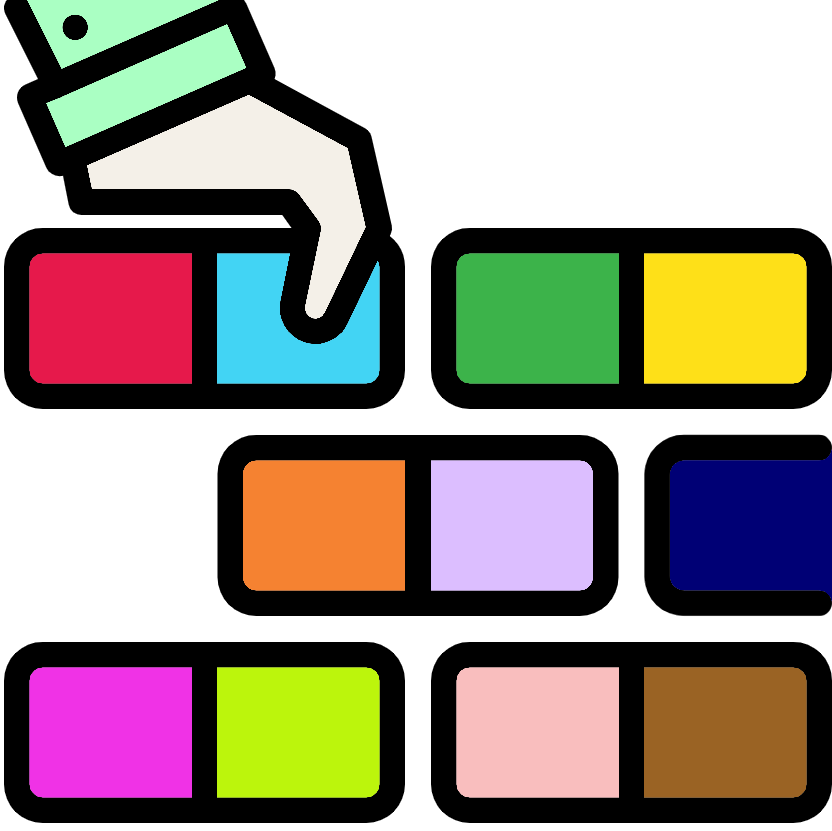
\includegraphics[width=0.2\linewidth]{figures/foundational} \end{center}

This week will cover the foundations of R. Understanding these concepts
is fundamental to becoming an R user. We'll start with
\textbf{operators}, these include \_\_+, -, *, and /\_\_, they allow us
to use R like a calculator. Then we will look at \textbf{variables}.
\textbf{Variables} allow us to save the output from commands so we can
use it in future commands.

A lot of the power of R comes from the vast array of \textbf{functions}
it contains. We will therefore look at some useful \textbf{functions} to
see the how they work. We will then look at how to interact with
directories in R.

We will end on some ways to use RStudio and the \textbf{script editor}.

\section{Operators}\label{operators}

\begin{center}
\includegraphics[width=0.2\linewidth]{figures/calculator} \end{center}

\textbf{Operators} are symbols in R that allow you to carry out many
common tasks. The 3 main types of \textbf{operators} in R are
arithmetic, logical, and bitwise. We will ignore logical and bitwise and
have a look at some arthimetic \textbf{operators}.

The four most commonly used arthimetic \textbf{opertors} are:

\begin{itemize}
\tightlist
\item
  \texttt{+} : Addition
\item
  \texttt{-} : Minus
\item
  \texttt{/} : Divide
\item
  \texttt{*} : Multiply
\end{itemize}

Run the following commands in your RStudio \textbf{console}.

\textbf{Note:} Each line below represents one command. Once a command is
typed out press enter to run the command.

\textbf{Note:} The amount of space between the integers/numbers and an
operator does not matter. It is a matter of preference and clarity.

\begin{Shaded}
\begin{Highlighting}[]
\DecValTok{2}\OperatorTok{+}\DecValTok{2}
\DecValTok{7}\OperatorTok{-}\DecValTok{7}
\DecValTok{10}\OperatorTok{/}\DecValTok{5}
\DecValTok{3}\OperatorTok{*}\DecValTok{3}
\DecValTok{6}\OperatorTok{+}\DecValTok{2}\OperatorTok{+}\DecValTok{4}
\DecValTok{8}\OperatorTok{-}\DecValTok{1}\OperatorTok{-}\DecValTok{3}
\end{Highlighting}
\end{Shaded}

R follows the BODMAS rules (Brackets, Orders (powers/roots), Division,
Multiplication, Addition, Subtraction). Try out the following commands
to demonstrate the usefulness of brackets.

\begin{Shaded}
\begin{Highlighting}[]
\DecValTok{3} \OperatorTok{+}\StringTok{ }\DecValTok{2} \OperatorTok{*}\StringTok{ }\DecValTok{2}\OperatorTok{/}\DecValTok{5}
\NormalTok{((}\DecValTok{3}\OperatorTok{+}\DecValTok{2}\NormalTok{) }\OperatorTok{*}\StringTok{ }\DecValTok{2}\NormalTok{) }\OperatorTok{/}\StringTok{ }\DecValTok{5}
\DecValTok{3} \OperatorTok{-}\StringTok{ }\DecValTok{2}\OperatorTok{*}\DecValTok{4} \OperatorTok{+}\StringTok{ }\DecValTok{1}
\NormalTok{(}\DecValTok{3}\OperatorTok{-}\DecValTok{2}\NormalTok{) }\OperatorTok{*}\StringTok{ }\NormalTok{(}\DecValTok{4}\OperatorTok{+}\DecValTok{1}\NormalTok{)}
\DecValTok{3} \OperatorTok{*}\StringTok{ }\DecValTok{3}\OperatorTok{/}\DecValTok{2} \OperatorTok{*}\StringTok{ }\DecValTok{2} \OperatorTok{-}\StringTok{ }\DecValTok{1}
\NormalTok{(}\DecValTok{3}\OperatorTok{*}\DecValTok{3}\NormalTok{) }\OperatorTok{/}\StringTok{ }\NormalTok{((}\DecValTok{2}\OperatorTok{*}\DecValTok{2}\NormalTok{) }\OperatorTok{-}\StringTok{ }\DecValTok{1}\NormalTok{)}
\end{Highlighting}
\end{Shaded}

When entering commands via the \textbf{console} the results/output is
printed to the screen (ignore the {[}1{]} at the moment). However, this
is no better than a normal calculator currently. R is a lot more
powerful as we shall see.

\section{Variables}\label{variables}

\begin{center}
\includegraphics[width=0.2\linewidth]{figures/boxes} \end{center}

The output/result of a command can be saved as a \textbf{variable}.
Below is the format for creating a \textbf{variable} in R (don't type
this into R).

\begin{Shaded}
\begin{Highlighting}[]
\NormalTok{variable_name <-}\StringTok{ }\NormalTok{variable_object}
\end{Highlighting}
\end{Shaded}

There are 3 parts to the above:

\begin{itemize}
\tightlist
\item
  The \textbf{variable name} (\texttt{variable\_name}). This is the name
  of the \textbf{variable} and is what will be used to refer to the
  \textbf{variable} in future commands. This name can be almost
  anything. There are some rules on what can be in a name:

  \begin{itemize}
  \tightlist
  \item
    Must start with a letter.
  \item
    Cannot contain spaces.
  \item
    Cannot start with a number.
  \item
    Cannot share the same name as a command or function in R.
  \item
    They are case sensitive. The \textbf{variable} name \texttt{BB} is
    differnet to the \textbf{variable} name \texttt{bb} which is
    differnet again to \texttt{bB}. I find it easiest to keep
    \textbf{variable names} in lower case.
  \end{itemize}
\item
  \texttt{\textless{}-} is called the assignment \textbf{operator}. It
  assigns the \textbf{variable object} to the \textbf{variable name}.

  \begin{itemize}
  \tightlist
  \item
    Tip you can press `ALT'+ `-' after a \textbf{variable name} as a
    shortcut for the assignment \textbf{operator}.
  \end{itemize}
\item
  The \textbf{variable object} (\texttt{variable\_object}). This can be
  many differnet objects including the output/results from commands,
  strings/words, numbers, and many other R data types.
\end{itemize}

A \textbf{variable} can be thought of as a box. The \textbf{variable
object} is held in the box but it can be replaced with any another
object. The \textbf{variable name} can then be thought as the label on
the box so you can tell which box is which.

Type the below commands into the RStudio \textbf{console}.

\textbf{Note.} Remember the amount of spaces between \textbf{operators}
and \textbf{integers} does not matter. I encourage you to experiment
with this spacing so you find what is best for you in terms of ease and
clarity.

\begin{Shaded}
\begin{Highlighting}[]
\NormalTok{bakers_dozen <-}\StringTok{ }\DecValTok{13}
\NormalTok{kilobyte <-}\StringTok{ }\DecValTok{1024}
\NormalTok{I <-}\StringTok{ }\DecValTok{1}
\NormalTok{II <-}\StringTok{ }\NormalTok{I }\OperatorTok{+}\StringTok{ }\DecValTok{1}
\NormalTok{V <-}\StringTok{ }\DecValTok{7} \OperatorTok{-}\StringTok{ }\NormalTok{II}
\NormalTok{X <-}\StringTok{ }\NormalTok{(II }\OperatorTok{/}\StringTok{ }\NormalTok{I) }\OperatorTok{*}\StringTok{ }\NormalTok{V}
\NormalTok{L <-}\StringTok{ }\NormalTok{X }\OperatorTok{*}\StringTok{ }\NormalTok{V}
\end{Highlighting}
\end{Shaded}

In the above commands the \textbf{variables} are not printed out to the
screen, this is as it should be. The \textbf{variables} are appearing in
the \textbf{environment} pane (Top right). This is very convenient to
see what variables are currently in the \textbf{environment} and to see
what they contain.

To print the contents of a \textbf{variable} to screen you can type the
\textbf{variable name} into the \textbf{console} and press enter. This
will print the \textbf{variable object} to the screen. This is not
needed for small \textbf{variable objects}, for which you can look at
the \textbf{environment} pane, but is useful for larger \textbf{variable
objects}.

\section{Functions}\label{functions}

\begin{center}
\includegraphics[width=0.2\linewidth]{figures/function} \end{center}

R \textbf{Functions} allow the user to carry out a specific task. R has
many inbuilt \textbf{functions} but you can also create your own.
Currently we will look at in built functions.

The basic layout of a \textbf{function} is:

\begin{Shaded}
\begin{Highlighting}[]
\KeywordTok{function_name}\NormalTok{(objects, options)}
\end{Highlighting}
\end{Shaded}

There are 3 main parts to the above:

\begin{itemize}
\tightlist
\item
  The \textbf{function name} (\texttt{function\_name})
\item
  The \textbf{object/s} to provide to the \textbf{function}.

  \begin{itemize}
  \tightlist
  \item
    This can be numbers, strings, \textbf{variables} we have created
    etc.
  \item
    Most \textbf{functions} require at least one \textbf{object}.
  \item
    Some \textbf{functions} can take multiple objects, if multiple
    \textbf{objects} are provided they must be seperated by \texttt{,}.
  \end{itemize}
\item
  \textbf{Function} options (\texttt{options}). Options can be provided
  to some \textbf{functions} to alter the way they will work.

  \begin{itemize}
  \tightlist
  \item
    Some \textbf{functions} don't have options.
  \item
    Most options have default modes. If the options is not specified the
    default mode will be used.
  \item
    Like \textbf{objects}, if using multiple options they must be
    sperated by \texttt{,}.
  \end{itemize}
\end{itemize}

Try running the below commands in your Rstudio \textbf{console}.

\begin{Shaded}
\begin{Highlighting}[]
\KeywordTok{ceiling}\NormalTok{(}\FloatTok{3.5}\NormalTok{)}
\KeywordTok{floor}\NormalTok{(}\FloatTok{3.5}\NormalTok{)}
\KeywordTok{sqrt}\NormalTok{(}\DecValTok{9}\NormalTok{)}
\KeywordTok{round}\NormalTok{(}\FloatTok{3.5555}\NormalTok{, }\DataTypeTok{digits =} \DecValTok{2}\NormalTok{)}
\KeywordTok{round}\NormalTok{(}\FloatTok{3.5555}\NormalTok{, }\DataTypeTok{digits =} \DecValTok{3}\NormalTok{)}
\KeywordTok{round}\NormalTok{(}\FloatTok{3.5555}\NormalTok{, }\DataTypeTok{digits =} \DecValTok{0}\NormalTok{)}
\NormalTok{two <-}\StringTok{ }\KeywordTok{sqrt}\NormalTok{(}\DecValTok{4}\NormalTok{)}
\end{Highlighting}
\end{Shaded}

The help page of \textbf{functions} can be accessed in 2 main ways:

\begin{itemize}
\tightlist
\item
  Click on the \textbf{function name} so your cursor is in it and press
  \textbf{F1}.
\item
  Type \texttt{?} followed by the \textbf{function name}. Example below:
\end{itemize}

\begin{Shaded}
\begin{Highlighting}[]
\NormalTok{?ceiling}
\end{Highlighting}
\end{Shaded}

\section{Directories}\label{directories}

\begin{center}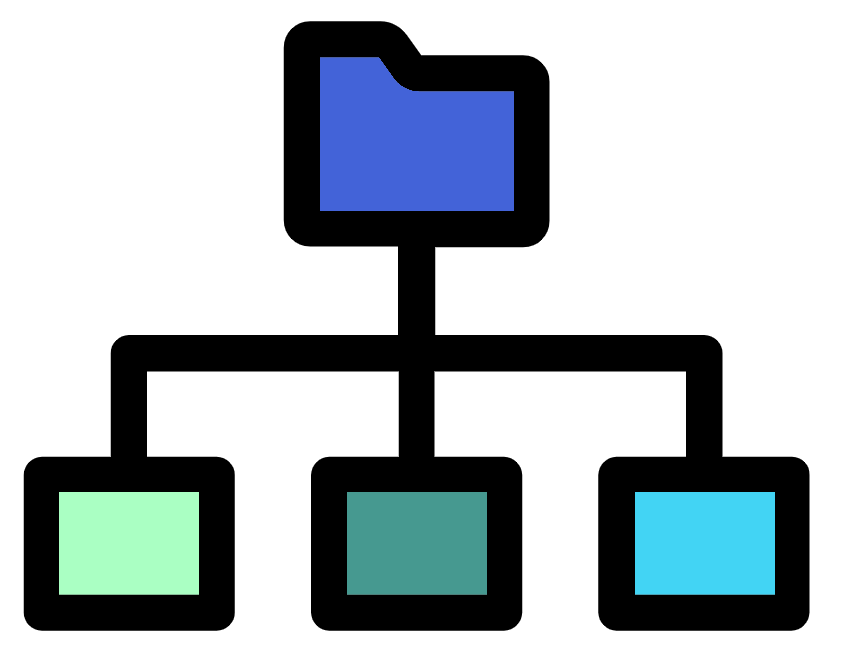
\includegraphics[width=0.2\linewidth]{figures/directories} \end{center}

It is important to know what directory you are working in and how to
change to different directories.

\subsection{Commands}\label{commands}

Below are commands you can run in the RStudio \textbf{console} or
\textbf{script editor} (use of script editor will be taught soon).

\begin{itemize}
\tightlist
\item
  Determine what directory you are currently in:
\end{itemize}

\begin{Shaded}
\begin{Highlighting}[]
\KeywordTok{getwd}\NormalTok{()}
\end{Highlighting}
\end{Shaded}

\begin{itemize}
\tightlist
\item
  Set working directory. The path of the directory must be in quotes
  like below. If you do run the below command make sure the path exists
  in your computer, as I am the sure the example below will not.
\end{itemize}

\begin{Shaded}
\begin{Highlighting}[]
\KeywordTok{setwd}\NormalTok{(}\StringTok{"/path/of/directory"")}
\end{Highlighting}
\end{Shaded}

\begin{itemize}
\tightlist
\item
  List the files in the current directory:
\end{itemize}

\begin{Shaded}
\begin{Highlighting}[]
\KeywordTok{list.files}\NormalTok{()}
\end{Highlighting}
\end{Shaded}

\subsection{RStudio Interface}\label{rstudio-interface}

The RStudio interface can also be used to carry out the above tasks.

To see what the current working directory is, you can look at the top
bar of the \textbf{console window}. The below shows I am in the
\textbf{``F:/R/CE/CE\_R\_for\_Everyone''} directory.

\begin{center}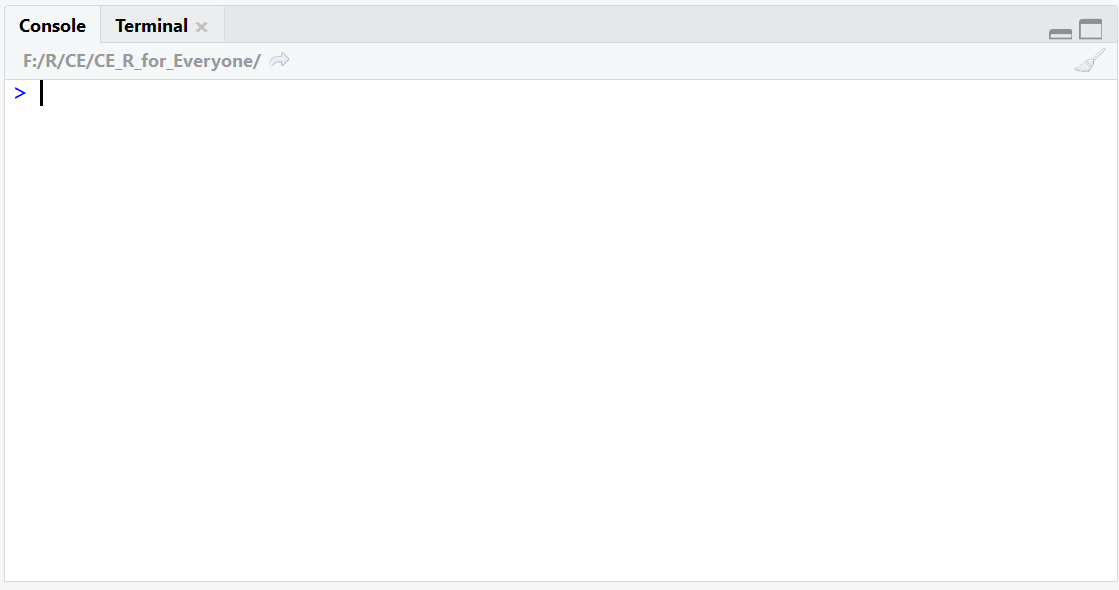
\includegraphics[width=0.6\linewidth]{figures/current_wd} \end{center}

There are two main ways to set your working directory.

\begin{enumerate}
\def\labelenumi{\arabic{enumi}.}
\tightlist
\item
  Via the tool bar:

  \begin{enumerate}
  \def\labelenumii{\arabic{enumii}.}
  \tightlist
  \item
    Click \textbf{``Session''}
  \item
    Go to the \textbf{``Set Working Directory''} drop down section
  \item
    Click \textbf{``Choose Directory..''}
  \item
    Use the pop-up browser to choose a directory
  \end{enumerate}
\item
  Via the \textbf{MISC window} (bottom left)

  \begin{enumerate}
  \def\labelenumii{\arabic{enumii}.}
  \tightlist
  \item
    Click the \textbf{Files pane}
  \item
    Navigate to the directory you would like to set as the working
    directory
  \item
    On the \textbf{MISC toolbar} click \textbf{``More''}
  \item
    On the drop down click \textbf{``Set As Working Directory''}
  \end{enumerate}
\end{enumerate}

To show the current working directory in the \textbf{Files} pane click
the arrow on the top bar of the \textbf{console window}. You can then
see what files and directories are in your working directory via the
\textbf{Files} pane in the \textbf{MISC} window.

\begin{center}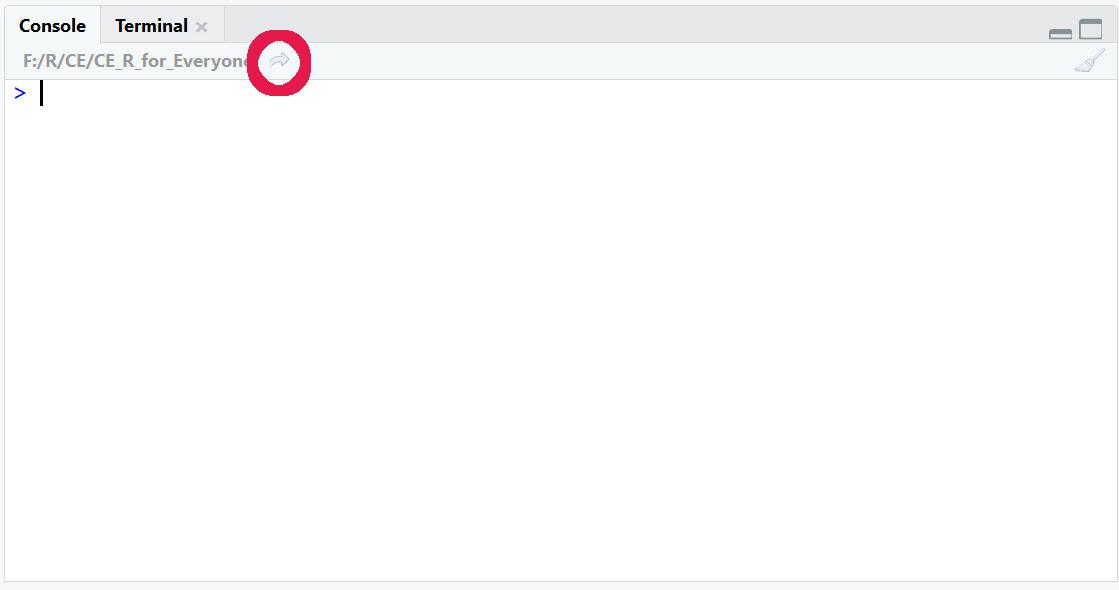
\includegraphics[width=0.8\linewidth]{figures/see_files} \end{center}

With this information create a directory you will use for this course.
This can be done outside of Rstudio or you can use the \textbf{Files
pane} in the \textbf{MISC window}. Once this is created set your working
directory to it. With that done we can go onto the next section.

\section{Script editor}\label{script-editor}

\begin{center}
\includegraphics[width=0.2\linewidth]{figures/editor} \end{center}

You can quickly type and run code using the \textbf{console window}.
However, to fully utilse Rstudio we will instead use the \textbf{script
editor} in the \textbf{source window}. This allows us to reuse and edit
code easier and it allows us to save our code so we can come back to it.

If you cannot see your \textbf{script editor}, click the multi window
button on the top of the \textbf{source window} or \textbf{console
window}.

\begin{center}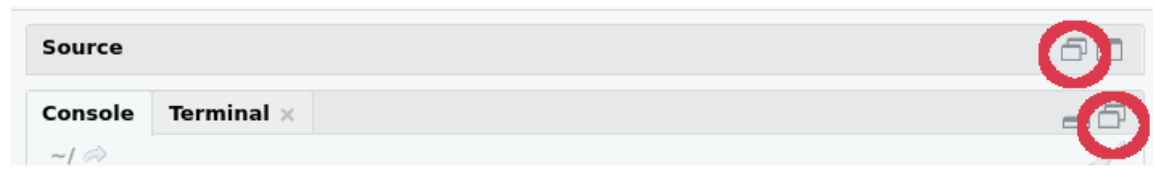
\includegraphics[width=0.8\linewidth]{figures/script_editor_expand} \end{center}

Type the below into the \textbf{script editor} and press
\textbf{``enter''}.

\begin{Shaded}
\begin{Highlighting}[]
\DecValTok{2} \OperatorTok{+}\StringTok{ }\DecValTok{2}
\end{Highlighting}
\end{Shaded}

Pressing enter goes to a new line without running the command, just like
other text editors (word, emails etc.).

On the new line type the below:

\begin{Shaded}
\begin{Highlighting}[]
\DecValTok{4} \OperatorTok{-}\StringTok{ }\DecValTok{1}
\end{Highlighting}
\end{Shaded}

\subsection{Running commands}\label{running-commands}

\begin{center}
\includegraphics[width=0.2\linewidth]{figures/command} \end{center}

You can run a command that is in the script editor by one of the two
following ways:

\begin{itemize}
\tightlist
\item
  Via cursor:

  \begin{itemize}
  \tightlist
  \item
    Move the cursor to the line you would like to run.
  \item
    Press \textbf{``Ctrl'' + ``enter''} ( \textbf{``cmd''} +
    \textbf{``enter''} for Mac)
  \end{itemize}
\item
  Highlighting:

  \begin{itemize}
  \tightlist
  \item
    Highlight the parts you would like and press \textbf{``Ctrl'' +
    ``enter''} ( \textbf{``cmd''} + \textbf{``enter''} for Mac)
  \item
    You can highlight a part of a line, a whole line, and even multiple
    lines.
  \end{itemize}
\end{itemize}

Run the commands you currently have in your \textbf{script editor}.

The \textbf{script editor} is unaffected with only the cursor moving if
you used the cursor method. Instead what is actually happening is your
commands are being copied to the \textbf{console window} and are being
run there.

I would encourage to primarily use the script editor to write your code.
It is brilliant for editing, reusing, and documenting your code.

\subsection{Annotations}\label{annotations}

\begin{center}
\includegraphics[width=0.2\linewidth]{figures/hashtag} \end{center}

Annotations can be added to your code in the \textbf{script editor}. If
a line starts with a \texttt{\#} it will not be run as a command, this
line is then an annotation. This is extremely useful to leave
information for your future self. It is much harder to go back to old
code and figure out what it does if it is just code.

Be a mate, annotate.

Edit the contents of your \textbf{script editor} so it looks like below.
Then run all the lines.

\textbf{Tip}: If you have selected the \textbf{script editor} you can
use \textbf{``Ctrl''} + \textbf{``a''} to highlight all.

\begin{Shaded}
\begin{Highlighting}[]
\CommentTok{#Command 1}
\DecValTok{2} \OperatorTok{+}\StringTok{ }\DecValTok{2}
\CommentTok{#Command 2}
\DecValTok{4} \OperatorTok{-}\StringTok{ }\DecValTok{1}
\end{Highlighting}
\end{Shaded}

\subsection{Saving scripts}\label{saving-scripts}

\begin{center}
\includegraphics[width=0.2\linewidth]{figures/r_save} \end{center}

Finally, one of the best aspects of using the \textbf{script editor} is
that you can save your scripts. I use this so I can have scripts for
specific projects and template scripts for certain tasks I routinely
carry out.

\begin{itemize}
\tightlist
\item
  To save a script you can click the floppy disk on the toolbar of the
  \textbf{source window}.
\item
  To save as, go to the RStudio toolbar and click \textbf{``File''}
  \textgreater{} \textbf{``Save As\ldots{}''}.
\end{itemize}

\subsection{Open a saved script}\label{open-a-saved-script}

You can open a previously saved script in 2 main ways:

\begin{itemize}
\tightlist
\item
  Via the \textbf{Files pane} in the \textbf{MISC window}

  \begin{itemize}
  \tightlist
  \item
    Navigate to the directory with the script (you do not need to set
    the working directory to this directory)
  \item
    Click the name of the script you would like to open
  \end{itemize}
\item
  Via the Rstudio toolbar

  \begin{itemize}
  \tightlist
  \item
    Click \textbf{``File''}
  \item
    Click \textbf{``Open file''}
  \item
    With the popup browser navigate to the location of the script and
    open it
  \end{itemize}
\end{itemize}

\subsection{New script}\label{new-script}

You can have multiple scripts open at one time and switch between these
scripts with the tabs at the top of the \textbf{script editor window}.

To create and open a new script, click on the button on the RStudio
toolbar shown below and select \textbf{``R script''}.

\begin{center}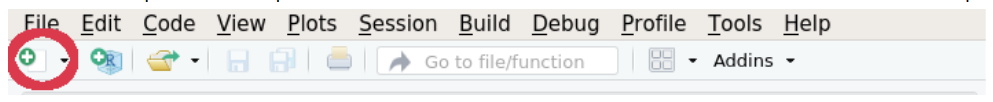
\includegraphics[width=0.8\linewidth]{figures/new_script_button} \end{center}

\chapter{Week 1 exercises}\label{week-1-exercises}

\begin{center}
\includegraphics[width=0.2\linewidth]{figures/kettle_bell} \end{center}

This will be the simplest of the weekly exercises but will be a good
oppurtunity to reinforce what you have learnt. In fact there is no
solution section for this week as it is unneeded.

The first task is to add the below text annotation to the top of your
current script.

\begin{Shaded}
\begin{Highlighting}[]
\CommentTok{# Foundations ####}
\end{Highlighting}
\end{Shaded}

Now save the file as \textbf{``Week1\_practice.R''} within the course
directory.

For the next part you will need to create a new script and save it as
\textbf{``Exercises.R''}.

On the first line of this script type the following annotation:

\begin{Shaded}
\begin{Highlighting}[]
\CommentTok{# Exercise 1 ####}
\end{Highlighting}
\end{Shaded}

The \texttt{\#\#\#\#} creates a code section, these will be explained in
a later week. You could also \texttt{-\/-\/-\/-} or \texttt{====} at the
end of an annotation to create a code section.

The next step is the most tedious, unfortunately tedious repetition is
one of the best ways to learn.

Please fill in the \textbf{``Exercises.R''} script with the commands
from the \textbf{operators} and \textbf{variables} section from chapter
2. Additionally, add in annotations so you can easily tell which
sections the commands come from and brief lines on their purposes.

Annotations require a balance of enough info but not too much info, you
don't always need a line of annotation for each line of code. However,
with some complex code sometimes you will need multiple lines of
annotattion for one line of code. It is all about how much annotation
you and possibly others will need for the code at hand. Knowing this
requires experience.

Next save the script, ensuring it is called
\textbf{``Day1\_Exercises.R''}"

Finally, close your script by clicking the \textbf{``x''}" icon on the
tab of the script.

That is the end of Week 1! If you have any questions please ask me
(Matthew Gemmell) and I am more than happy to try to answer.

\chapter{Week 2 - R objects}\label{week-2---r-objects}

\begin{center}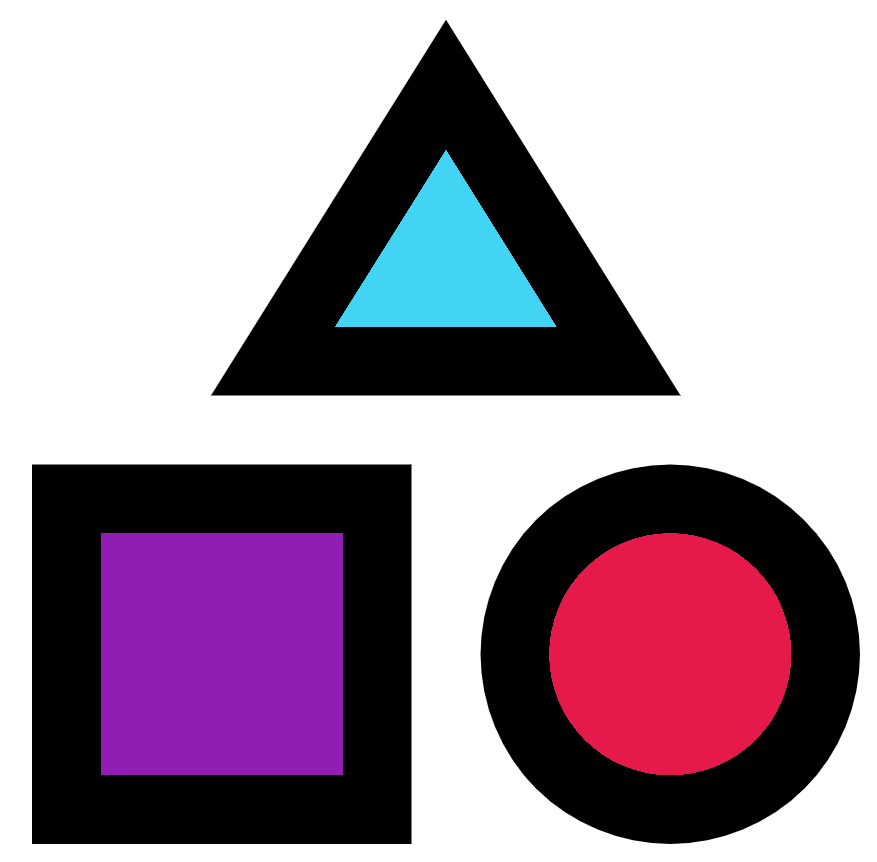
\includegraphics[width=0.2\linewidth]{figures/RObjects} \end{center}

Last week we learnt how to create a \textbf{variable}. This consisted of
assigning (\texttt{\textless{}-}) an \textbf{object} a name. This week
we will learn about \textbf{R objects}. There are two major R
terminologies to learn to fully understand \textbf{R objects}.

\begin{itemize}
\tightlist
\item
  \textbf{Class}: An \textbf{R object} will have a specific class. The
  \textbf{class} determines what the \textbf{object} is. It could be
  numbers, text, or other types of \textbf{classess}.
\item
  \textbf{Data structure}: This determines the structure of an \textbf{R
  object}.
\end{itemize}

Today's plan is to learn about \textbf{classes} and \textbf{data
structures}.

\section{Code sections}\label{code-sections}

Today, and for the rest of the course, you will use code sections in
your R scripts to seperate sections in this book.

First set your working directory to the course directory, create a
script, and save it as \textbf{``Week2\_practice.R''}.

Next create a code section at the top of this script called
\textbf{``Classes''}.

In other words have the below at the top of your script:

\begin{Shaded}
\begin{Highlighting}[]
\CommentTok{# Classes ####}
\end{Highlighting}
\end{Shaded}

\section{Classes}\label{classes}

There are six basic \textbf{classes} in R (Also known as the
\textbf{atomic classes}).

The four we will learn are:

\begin{itemize}
\tightlist
\item
  \textbf{Integer}
\item
  \textbf{Double}
\item
  \textbf{String}
\item
  \textbf{Logical}.
\end{itemize}

There are also the classes \textbf{complex} and \textbf{raw}.

\subsection{Numeric}\label{numeric}

\begin{center}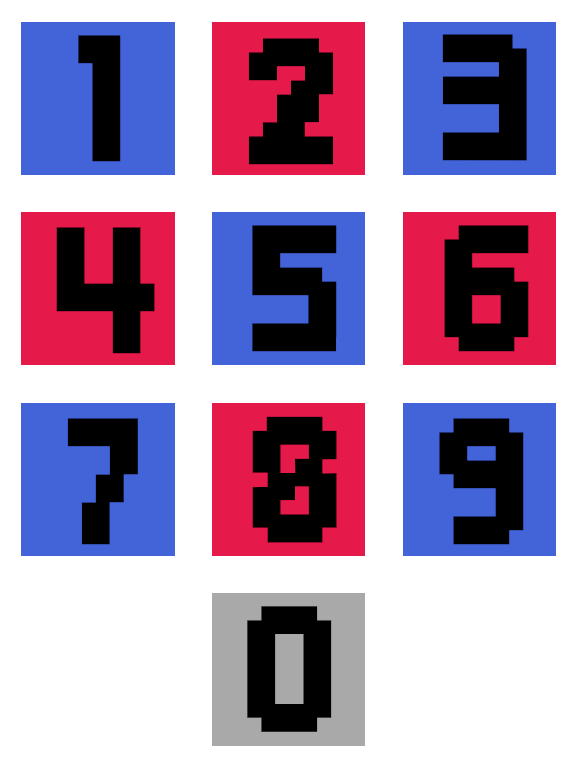
\includegraphics[width=0.2\linewidth]{figures/numbers} \end{center}

\textbf{Numeric} \textbf{classes} come in two types, \textbf{integer}
and \textbf{double}. \textbf{Integers} and \textbf{doubles} are almost
identical. However, \textbf{doubles} contain decimal point information
whilst \textbf{integers} do not.

Most of the time you will only need to know if your data is
\textbf{numeric} and you will not need to worry about \textbf{doubles}
or \textbf{integers}. The exception being if you are working with
decimals and your decimals are not showing up. This probably means that
your \textbf{object} has the \textbf{integer class}.

Type and run the following, using the provided annotation to understand
what the commands are doing.

\textbf{Note:} Remember you can copy and paste old script.

Use the \textbf{function} \texttt{class()} to show the \textbf{class} of
an R \textbf{object}:

\begin{Shaded}
\begin{Highlighting}[]
\CommentTok{#Numeric}
\CommentTok{#Class of 2}
\KeywordTok{class}\NormalTok{(}\DecValTok{2}\NormalTok{)}
\CommentTok{#class of 3.14}
\KeywordTok{class}\NormalTok{(}\FloatTok{3.14}\NormalTok{)}
\CommentTok{#class of 6}
\KeywordTok{class}\NormalTok{(}\DecValTok{6}\NormalTok{)}
\end{Highlighting}
\end{Shaded}

Create a \textbf{variable} with the \textbf{name} ``pie''" containing
the \textbf{numeric} 3.14:

\begin{Shaded}
\begin{Highlighting}[]
\CommentTok{#Creating a variable using the assignment operator}
\NormalTok{pie <-}\StringTok{ }\FloatTok{3.14}
\end{Highlighting}
\end{Shaded}

Use the \textbf{functions} \texttt{as.numeric()}, \texttt{as.integer()},
\texttt{as.double()} to print the \textbf{variable} as a
\textbf{numeric}, as an \textbf{integer}, and as a \textbf{double}:

\begin{Shaded}
\begin{Highlighting}[]
\CommentTok{#Printing out previously made variable as numeric, integer, and double}
\KeywordTok{as.numeric}\NormalTok{(pie)}
\KeywordTok{as.integer}\NormalTok{(pie)}
\KeywordTok{as.double}\NormalTok{(pie)}
\end{Highlighting}
\end{Shaded}

You can put a \textbf{function} as the \textbf{variable} within a
\textbf{function}.

Below we will first check the \textbf{class} of the \textbf{object}
within the ``pie'' \textbf{variable}. You will note that the
\textbf{functions} we used previously did not permanently change the
\textbf{variable's object}. We can only change a \textbf{variable} if we
use the \textbf{assignment operator}.

Then we will check the \textbf{class} of the \textbf{object} as it is
altered by the various \texttt{as.} \textbf{functions}.

\begin{Shaded}
\begin{Highlighting}[]
\CommentTok{#Checking the class of our variable}
\KeywordTok{class}\NormalTok{(pie)}
\KeywordTok{class}\NormalTok{(}\KeywordTok{as.numeric}\NormalTok{(pie))}
\KeywordTok{class}\NormalTok{(}\KeywordTok{as.integer}\NormalTok{(pie))}
\KeywordTok{class}\NormalTok{(}\KeywordTok{as.double}\NormalTok{(pie))}
\end{Highlighting}
\end{Shaded}

\textbf{Note:} Remember to ask for help if you need it!

On a side note, R comes with some inbuilt variables such as pi:

\begin{Shaded}
\begin{Highlighting}[]
\CommentTok{#The R pi is equal to 3.141593}
\NormalTok{pi}
\CommentTok{#assign pi to 3.14}
\NormalTok{pi <-}\StringTok{ }\FloatTok{3.14}
\CommentTok{#print out pi to see you have changed the variable's object}
\NormalTok{pi}
\CommentTok{#in this case if you want the original R pi object back, we can remove the one we made}
\KeywordTok{rm}\NormalTok{(pi)}
\end{Highlighting}
\end{Shaded}

Have you been annotating your scripts?

\subsection{Logical}\label{logical}

\begin{center}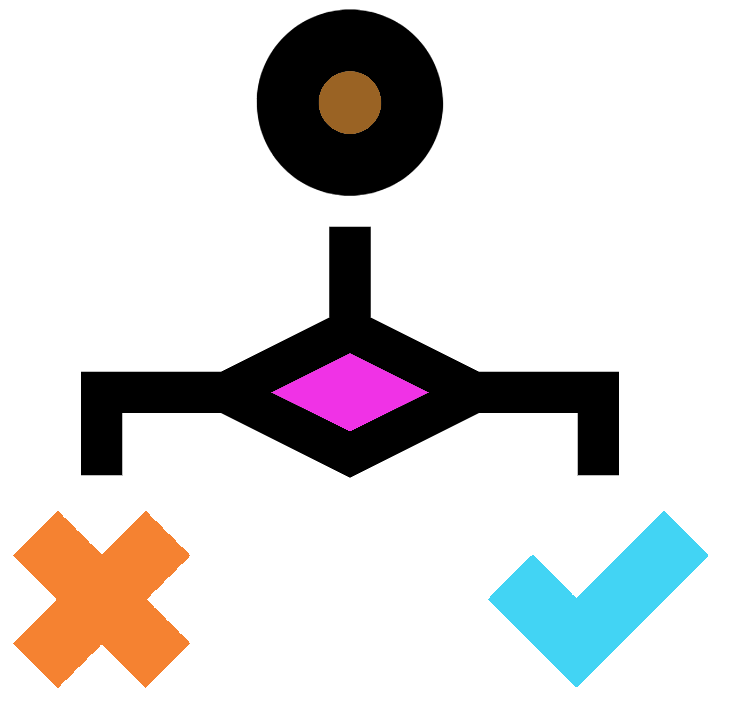
\includegraphics[width=0.2\linewidth]{figures/logical} \end{center}

\textbf{Logical} values can be \textbf{TRUE} or \textbf{FALSE}.

They are primarily used when comparing objects.

Run the below commands to output \textbf{Logical} values using the
various \textbf{logical operators}.

Note: when \texttt{!} is used in \textbf{operators} it means ``not''.
When used, \texttt{!} always goes at the front of the operator.

\begin{Shaded}
\begin{Highlighting}[]
\CommentTok{#Logical}
\CommentTok{# 2 less than 4 }
\DecValTok{2} \OperatorTok{<}\StringTok{ }\DecValTok{2}
\CommentTok{# 2 greater than 4}
\DecValTok{2} \OperatorTok{>}\StringTok{ }\DecValTok{2}
\CommentTok{# 2 less than or equal to 4}
\DecValTok{2} \OperatorTok{<=}\StringTok{ }\DecValTok{4}
\CommentTok{# greater than or equal}
\DecValTok{2} \OperatorTok{>=}\StringTok{ }\DecValTok{2}
\CommentTok{# equal}
\DecValTok{2} \OperatorTok{==}\StringTok{ }\DecValTok{4}
\CommentTok{# not equal}
\DecValTok{2} \OperatorTok{!=}\StringTok{ }\DecValTok{4}
\end{Highlighting}
\end{Shaded}

It is probably not immediately obvious how useful \textbf{logicals} but
you'll see how they are later in the course.

\subsection{String}\label{string}

\begin{center}
\includegraphics[width=0.2\linewidth]{figures/string_bubble} \end{center}

\textbf{Strings} are text and can be modified in R in ways you would
normaly want to modify text. They are called \textbf{strings} as they
are strings of characters. \textbf{Strings} are flanked by quote marks.
Double quotes (\texttt{""}) are prefferred but single quotes can also be
used (\texttt{\textquotesingle{}\textquotesingle{}}).

Type and run the below examples to get some practice with
\textbf{strings}.

A \textbf{string object} can consist of a string containing one
\textbf{character}:

\begin{Shaded}
\begin{Highlighting}[]
\CommentTok{#String}
\NormalTok{one_character_string <-}\StringTok{ "A"}
\NormalTok{one_character_string}
\end{Highlighting}
\end{Shaded}

A \textbf{string object} can consist of a string containing multiple
\textbf{characters}:

\begin{Shaded}
\begin{Highlighting}[]
\NormalTok{word_string <-}\StringTok{ "alphabet"}
\NormalTok{word_string}
\end{Highlighting}
\end{Shaded}

A \textbf{string} can contain all the different characters and any
number of them. The only exception is that if you try to put a double
quote in your string it will cause an issue.

\begin{Shaded}
\begin{Highlighting}[]
\NormalTok{long_string <-}\StringTok{ "Strings can be long and contain more than letters. }\CharTok{\textbackslash{}\textbackslash{}}\StringTok{.("}
\NormalTok{long_string}
\end{Highlighting}
\end{Shaded}

A \textbf{string} doesn't need letters, it can consist of only numbers.
Note the terms \textbf{string} and \textbf{character} can be used
interchangeably.

\begin{Shaded}
\begin{Highlighting}[]
\NormalTok{number_string <-}\StringTok{ "1066"}
\NormalTok{number_string}
\KeywordTok{class}\NormalTok{(number_string)}
\end{Highlighting}
\end{Shaded}

You can convert a \textbf{numeric} to a \textbf{string/character}.

\begin{Shaded}
\begin{Highlighting}[]
\NormalTok{number <-}\StringTok{ }\DecValTok{1066}
\NormalTok{numeric_to_string <-}\StringTok{ }\KeywordTok{as.character}\NormalTok{(number)}
\NormalTok{numeric_to_string}
\KeywordTok{class}\NormalTok{(numeric_to_string)}
\end{Highlighting}
\end{Shaded}

An appropriate \textbf{string} can be converted to a \textbf{numeric}.
This is useful as mathematical \textbf{operators} will not work with
\textbf{strings}.

\begin{Shaded}
\begin{Highlighting}[]
\CommentTok{#will get an error as strings and maths don't mix}
\StringTok{"6"} \OperatorTok{-}\StringTok{ }\DecValTok{3}
\CommentTok{#will work as maths and numerics work}
\KeywordTok{as.numeric}\NormalTok{(}\StringTok{"6"}\NormalTok{) }\OperatorTok{-}\StringTok{ }\DecValTok{4}
\CommentTok{#Below will not work as only strings containing numbers can be converted to numeric}
\KeywordTok{as.numeric}\NormalTok{(}\StringTok{"not_a_number_12"}\NormalTok{)}
\end{Highlighting}
\end{Shaded}

You can use certain \textbf{logical operators} to compare
\textbf{strings} though:

\begin{Shaded}
\begin{Highlighting}[]
\StringTok{"character"} \OperatorTok{==}\StringTok{ "character"}
\StringTok{"1066"} \OperatorTok{!=}\StringTok{ "character"}
\StringTok{"numeric"} \OperatorTok{==}\StringTok{ "string"}
\end{Highlighting}
\end{Shaded}

The \textbf{paste() function} is very useful to combine two or more
\textbf{strings} into one.

\begin{Shaded}
\begin{Highlighting}[]
\KeywordTok{paste}\NormalTok{(}\StringTok{"The following is a string:"}\NormalTok{, long_string) }
\KeywordTok{paste}\NormalTok{(number_string, }\StringTok{"is a"}\NormalTok{, word_string)}
\CommentTok{#By default paste will put a spaces between each string you provide}
\CommentTok{#You can use the sep option to specific your own}
\KeywordTok{paste}\NormalTok{(}\StringTok{"However"}\NormalTok{, }\StringTok{" this is seperated by a comma"}\NormalTok{, }\DataTypeTok{sep =} \StringTok{","}\NormalTok{)}
\CommentTok{#Or you can make it so there is no seperator}
\KeywordTok{paste}\NormalTok{(}\StringTok{"no seperator"}\NormalTok{,numeric_to_string, }\DataTypeTok{sep =} \StringTok{""}\NormalTok{)}
\end{Highlighting}
\end{Shaded}

\section{Code section continued}\label{code-section-continued}

After all that you will have some nice code and annotations in your
script editor for the \textbf{Classes} code section.

Making a code section is not very useful until you have multiple code
sections. To show this create a new code section at the bottom of your
script called \textbf{``Data structures''}. This new code section will
be used for the next section.

\begin{Shaded}
\begin{Highlighting}[]
\CommentTok{# Data structures ####}
\end{Highlighting}
\end{Shaded}

With the new code section created we can now see why code sections are
so useful. Go to the text that denotes the first code section
(\textbf{``Classes''}). Look between the numbers on the left that
signify the line number, and the text. You will see an arrow pointing
downwards. You can click that arrow and it will collapse the code
section. Click the arrow, now pointing right, and it will expand the
code section. This is super useful so you can hide code sections in your
script that you don't currently need to look at.

\begin{center}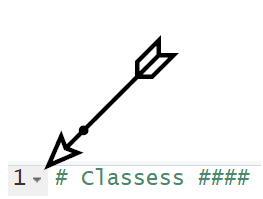
\includegraphics[width=0.2\linewidth]{figures/R_code_section_collapse} \end{center}

With the \textbf{``Classes''} code section collapsed let us continue to
the next section. There will be less annotations in this book as I
expect you will make your own now.

\section{Data structures}\label{data-structures}

\textbf{Data structures} describe how data is structured in an
\textbf{object}. We will go into 3 main types of \textbf{data
structures}.

\begin{itemize}
\tightlist
\item
  \textbf{Scalar}
\item
  \textbf{Vectors} \& \textbf{Lists}
\item
  \textbf{Matrices} \& \textbf{Data frames}
\end{itemize}

\subsection{Scalar}\label{scalar}

\begin{center}
\includegraphics[width=0.2\linewidth]{figures/Rscalar} \end{center}

A \textbf{scalar} consists of one value in an object. This can be one
\textbf{string}, one \textbf{numeric}, one \textbf{logical} etc. We have
only been working with \textbf{scalars} thus far but this is about to
change.

\subsection{Vectors \& Lists}\label{vectors-lists}

\begin{center}
\includegraphics[width=0.2\linewidth]{figures/Rvector} \end{center}

A \textbf{R object} can hold multiple values.Many \textbf{data}
structures can do this with the simplest being a \textbf{vector}.

A \textbf{vector} can be created with the \texttt{c()}
\textbf{function}. This function will combine the provided objects into
a single \textbf{vector} or \textbf{list}.

\textbf{Vectors} and \textbf{lists} are both 1-dimensional \textbf{data
structures}. \textbf{Vectors} can only contain one \textbf{class}
(homogeneous) whilst \textbf{lists} can contain multiple
(heterogeneous). There is more to \textbf{lists} but we will not go into
them.

Run the following commands to produce \textbf{variables} which contain
\textbf{vectors}.

\begin{Shaded}
\begin{Highlighting}[]
\NormalTok{number_vec <-}\StringTok{ }\KeywordTok{c}\NormalTok{(}\DecValTok{1}\NormalTok{,}\DecValTok{2}\NormalTok{,}\DecValTok{4}\NormalTok{,}\DecValTok{8}\NormalTok{,}\DecValTok{16}\NormalTok{)}
\NormalTok{number_vec}
\NormalTok{number_series_vec <-}\StringTok{ }\DecValTok{1}\OperatorTok{:}\DecValTok{6}
\NormalTok{number_series_vec}
\NormalTok{animals <-}\StringTok{ }\KeywordTok{c}\NormalTok{(}\StringTok{"Whale"}\NormalTok{,}\StringTok{"Seal"}\NormalTok{,}\StringTok{"Hedgehog"}\NormalTok{,}\StringTok{"Mouse"}\NormalTok{,}\StringTok{"Owl"}\NormalTok{,}\StringTok{"Squirrel"}\NormalTok{,}\StringTok{"Vole"}\NormalTok{,}\StringTok{"Shrew"}\NormalTok{)}
\NormalTok{animals}
\end{Highlighting}
\end{Shaded}

Elements of a \textbf{vector} can be accessed through their indices:

\begin{Shaded}
\begin{Highlighting}[]
\NormalTok{birds <-}\StringTok{ }\NormalTok{animals[}\DecValTok{5}\NormalTok{]}
\NormalTok{birds}
\NormalTok{aquatic <-}\StringTok{ }\NormalTok{animals[}\DecValTok{1}\OperatorTok{:}\DecValTok{2}\NormalTok{]}
\NormalTok{aquatic}
\NormalTok{rodents <-}\StringTok{ }\NormalTok{animals[}\KeywordTok{c}\NormalTok{(}\DecValTok{3}\NormalTok{,}\DecValTok{6}\NormalTok{,}\DecValTok{7}\NormalTok{)]}
\NormalTok{rodents}
\NormalTok{mammals <-}\StringTok{ }\NormalTok{animals[}\OperatorTok{-}\DecValTok{5}\NormalTok{]}
\NormalTok{mammals}
\end{Highlighting}
\end{Shaded}

You can use \textbf{operators} and \textbf{functions} on a
\textbf{vector}. When you do each \textbf{scalar} within the
\textbf{vector} will be acted upon.

\begin{Shaded}
\begin{Highlighting}[]
\NormalTok{number_vec }\OperatorTok{-}\StringTok{ }\DecValTok{1}
\NormalTok{number_vec }\OperatorTok{*}\StringTok{ }\DecValTok{2}
\KeywordTok{log}\NormalTok{(number_vec)}
\KeywordTok{length}\NormalTok{(rodents)}
\end{Highlighting}
\end{Shaded}

Some \textbf{functions} are specifically used for \textbf{vectors}:

\begin{Shaded}
\begin{Highlighting}[]
\KeywordTok{mean}\NormalTok{(number_vec)}
\KeywordTok{summary}\NormalTok{(number_vec)}
\end{Highlighting}
\end{Shaded}

We can also test the values within \textbf{vectors}:

\begin{Shaded}
\begin{Highlighting}[]
\NormalTok{aquatic }\OperatorTok{==}\StringTok{ "Whale"}
\NormalTok{number_vec }\OperatorTok{>}\StringTok{ }\DecValTok{4}
\NormalTok{number_vec[number_vec }\OperatorTok{>}\StringTok{ }\DecValTok{4}\NormalTok{]}
\end{Highlighting}
\end{Shaded}

The \texttt{paste()} \textbf{function} can be used to paste
\textbf{string scalars} to other \textbf{string scalars} or to
\textbf{string vectors}:

\begin{Shaded}
\begin{Highlighting}[]
\KeywordTok{paste}\NormalTok{(}\StringTok{"Animals"}\NormalTok{, animals)}
\NormalTok{bird_or_mammal <-}\StringTok{ }\KeywordTok{c}\NormalTok{(}\StringTok{"mammal"}\NormalTok{,}\StringTok{"mammal"}\NormalTok{,}\StringTok{"mammal"}\NormalTok{,}\StringTok{"mammal"}\NormalTok{,}\StringTok{"bird"}\NormalTok{,}\StringTok{"mammal"}\NormalTok{,}\StringTok{"mammal"}\NormalTok{,}\StringTok{"mammal"}\NormalTok{)}
\KeywordTok{paste}\NormalTok{(animals, bird_or_mammal, }\DataTypeTok{sep =} \StringTok{":"}\NormalTok{)}
\KeywordTok{paste}\NormalTok{(animals, }\StringTok{" is a "}\NormalTok{, bird_or_mammal, }\DataTypeTok{sep =} \StringTok{""}\NormalTok{)}
\end{Highlighting}
\end{Shaded}

\subsection{Data frames \& Matrices}\label{data-frames-matrices}

\begin{center}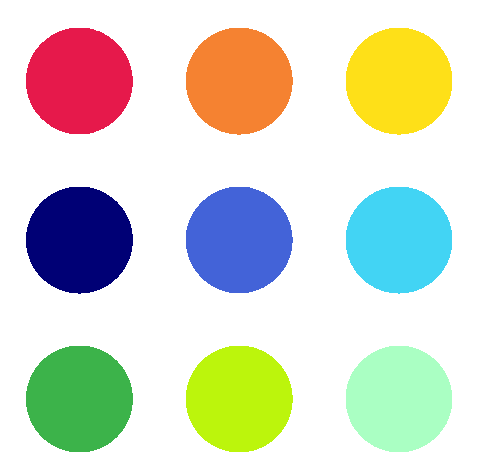
\includegraphics[width=0.2\linewidth]{figures/Rmatrix} \end{center}

\textbf{Data frames} \& \textbf{matrices} are 2-dimensional data
structures as they have rows and columns.

A \textbf{matrix} only contains 1 \textbf{class} (homogeneous). A
\textbf{data frame} can contain multiple classes (heterogenous), but
each column can only contain one \textbf{class}.

Most of the time \textbf{data frames} and \textbf{matrices} can be
treated the same. Because of this I generally use \textbf{data frames}
and so we will focus on them.

R comes with a set of pre-loaded data. If you are interested you can use
the \textbf{function} \texttt{data()} to see the full list.

We will have a quick look at the dataset ``mtcars''. This is a
\textbf{data frame} containing information on various cars. To look at
the \textbf{data frame} in the \textbf{console window} run the below.

\begin{Shaded}
\begin{Highlighting}[]
\NormalTok{mtcars}
\end{Highlighting}
\end{Shaded}

To get a better look save the \textbf{data frame} as a
\textbf{variable}. The above shows the info in the \textbf{console
window}. However we can have a better look at it in RStudio if we save
it as a variable in our \textbf{environment} and then click the variable
on the \textbf{Environment pane} of the \textbf{``environment and
history''} \textbf{window}.

\begin{Shaded}
\begin{Highlighting}[]
\NormalTok{cars_info <-}\StringTok{ }\NormalTok{mtcars}
\end{Highlighting}
\end{Shaded}

Now the \textbf{variable} will be listed in your \textbf{Environment
pane} in the \textbf{``environment and history'' window} . Click on the
name ``cars\_info'' in the \textbf{Environment pane}. A tab in your
\textbf{script editor} will open so you can have a good look at the
contents of the \textbf{data frame}.

When you are ready, close the ``cars\_info'' tab and remove the
\textbf{variable} with the below command.

\begin{Shaded}
\begin{Highlighting}[]
\KeywordTok{rm}\NormalTok{(cars_info)}
\end{Highlighting}
\end{Shaded}

Now it is time to create our own \textbf{data frame}.

First we will create three \textbf{variables} containing
\textbf{vectors}. These will be our three columns.

\begin{Shaded}
\begin{Highlighting}[]
\NormalTok{Crab <-}\StringTok{ }\KeywordTok{c}\NormalTok{(}\DecValTok{10}\NormalTok{,}\DecValTok{1}\NormalTok{,}\DecValTok{1}\NormalTok{)}
\NormalTok{Oystercatcher <-}\StringTok{ }\KeywordTok{c}\NormalTok{(}\DecValTok{5}\NormalTok{,}\DecValTok{6}\NormalTok{,}\DecValTok{4}\NormalTok{)}
\NormalTok{Starfish <-}\StringTok{ }\KeywordTok{c}\NormalTok{(}\DecValTok{3}\NormalTok{,}\DecValTok{3}\NormalTok{,}\DecValTok{7}\NormalTok{)}
\end{Highlighting}
\end{Shaded}

Now let us create the \textbf{data frame}.

\begin{Shaded}
\begin{Highlighting}[]
\CommentTok{#Using the function data.frame to create a data frame}
\NormalTok{beach_df <-}\StringTok{ }\KeywordTok{data.frame}\NormalTok{(Crab,Oystercatcher,Starfish)}
\end{Highlighting}
\end{Shaded}

Look at the \textbf{variable} ``beach\_df'' (it is useful to use ``df''
in \textbf{variable names} to signify it is a \textbf{data frame}) and
you will see that each \textbf{vector} has become a column. The
\textbf{variable names} have become the column names (this is why we
used capital letters in the \textbf{variable names}).

You can think of \textbf{data frames} in three differnet ways:

\begin{itemize}
\tightlist
\item
  A list of columns
\item
  A list of rows
\item
  A table
\end{itemize}

Look at the column and row names with two new \textbf{functions}.

\begin{Shaded}
\begin{Highlighting}[]
\KeywordTok{colnames}\NormalTok{(beach_df)}
\KeywordTok{row.names}\NormalTok{(beach_df)}
\end{Highlighting}
\end{Shaded}

We can use the \textbf{function} \texttt{row.names()} and the
\textbf{assignment operator} to change the row names to something more
useful.

\begin{Shaded}
\begin{Highlighting}[]
\KeywordTok{row.names}\NormalTok{(beach_df) <-}\StringTok{ }\KeywordTok{c}\NormalTok{(}\StringTok{"Formby"}\NormalTok{,}\StringTok{"West Kirby"}\NormalTok{,}\StringTok{"Crosby"}\NormalTok{)}
\end{Highlighting}
\end{Shaded}

Now look at your ``beach\_df'' \textbf{data frame} to see the
difference.

That is quite a lot to go through so let us reinforce it all with
exercise!

\chapter{Week 2 exercises}\label{week-2-exercises}

\begin{center}
\includegraphics[width=0.2\linewidth]{figures/beach} \end{center}

For this exercise simply produce the following tables as \textbf{data
frames} in R. Please carry this out in your \textbf{``Exercises.R''}
script and remember about code sections and annotations.

Tip: You can either write completely new code or reuse and alter
previous code.

\section{df}\label{df}

\textbf{Note}: The top row is the column names and the left-most column
is the row names.

\begin{tabular}{l|r|r|r}
\hline
  & One & Three & Five\\
\hline
Two & 2 & 6 & 10\\
\hline
Four & 4 & 12 & 20\\
\hline
Six & 6 & 18 & 30\\
\hline
\end{tabular}

\section{beach\_df\_2}\label{beach_df_2}

\textbf{Note}: The top row is the column names and the left-most column
is the row names.

\begin{tabular}{l|r|r|r|r}
\hline
  & Crab & Oystercatcher & Sandpiper & Starfish\\
\hline
Formby & 10 & 5 & 1 & 3\\
\hline
West Kirby & 1 & 6 & 1 & 3\\
\hline
Crosby & 1 & 4 & 2 & 7\\
\hline
New Brighton & 4 & 4 & 3 & 4\\
\hline
\end{tabular}

\chapter{Week 2 exercise solutions}\label{week-2-exercise-solutions}

\begin{center}
\includegraphics[width=0.2\linewidth]{figures/week2_solutions} \end{center}

\section{df solution}\label{df-solution}

\subsection{Step 1}\label{step-1}

Create \textbf{vectors} for columns and row names:

\begin{Shaded}
\begin{Highlighting}[]
\NormalTok{One <-}\StringTok{ }\KeywordTok{c}\NormalTok{(}\DecValTok{2}\NormalTok{,}\DecValTok{4}\NormalTok{,}\DecValTok{6}\NormalTok{)}
\NormalTok{Three <-}\StringTok{ }\KeywordTok{c}\NormalTok{(}\DecValTok{6}\NormalTok{,}\DecValTok{12}\NormalTok{,}\DecValTok{18}\NormalTok{)}
\NormalTok{Five <-}\StringTok{ }\KeywordTok{c}\NormalTok{(}\DecValTok{10}\NormalTok{,}\DecValTok{20}\NormalTok{,}\DecValTok{30}\NormalTok{)}
\NormalTok{row_names <-}\StringTok{ }\KeywordTok{c}\NormalTok{(}\StringTok{"Two"}\NormalTok{, }\StringTok{"Four"}\NormalTok{, }\StringTok{"Six"}\NormalTok{)}
\end{Highlighting}
\end{Shaded}

\subsection{Step 2a}\label{step-2a}

Create the \textbf{data frame} from vectors:

\begin{Shaded}
\begin{Highlighting}[]
\NormalTok{df <-}\StringTok{ }\KeywordTok{data.frame}\NormalTok{(One,Three,Five)}
\end{Highlighting}
\end{Shaded}

Add row names:

\begin{Shaded}
\begin{Highlighting}[]
\KeywordTok{row.names}\NormalTok{(df) <-}\StringTok{ }\NormalTok{row_names}
\end{Highlighting}
\end{Shaded}

\subsection{Step 2b}\label{step-2b}

Alternatively you can define the row names in the \texttt{data.frame()}
\texttt{function} as an option:

\begin{Shaded}
\begin{Highlighting}[]
\NormalTok{df <-}\StringTok{ }\KeywordTok{data.frame}\NormalTok{(One,Three,Five, }\DataTypeTok{row.names =}\NormalTok{ row_names)}
\end{Highlighting}
\end{Shaded}

\section{beach\_df\_2 solution}\label{beach_df_2-solution}

\subsection{Step 1}\label{step-1-1}

Create \textbf{vectors} for columns and row names:

\begin{Shaded}
\begin{Highlighting}[]
\NormalTok{Crab <-}\StringTok{ }\KeywordTok{c}\NormalTok{(}\DecValTok{10}\NormalTok{,}\DecValTok{1}\NormalTok{,}\DecValTok{1}\NormalTok{,}\DecValTok{4}\NormalTok{)}
\NormalTok{Oystercatcher <-}\StringTok{ }\KeywordTok{c}\NormalTok{(}\DecValTok{5}\NormalTok{,}\DecValTok{6}\NormalTok{,}\DecValTok{4}\NormalTok{,}\DecValTok{4}\NormalTok{)}
\NormalTok{Sandpiper <-}\StringTok{ }\KeywordTok{c}\NormalTok{(}\DecValTok{1}\NormalTok{,}\DecValTok{1}\NormalTok{,}\DecValTok{2}\NormalTok{,}\DecValTok{3}\NormalTok{)}
\NormalTok{Starfish <-}\StringTok{ }\KeywordTok{c}\NormalTok{(}\DecValTok{3}\NormalTok{,}\DecValTok{3}\NormalTok{,}\DecValTok{7}\NormalTok{,}\DecValTok{4}\NormalTok{)}
\NormalTok{row_names_}\DecValTok{2}\NormalTok{ <-}\StringTok{ }\KeywordTok{c}\NormalTok{(}\StringTok{"Formby"}\NormalTok{,}\StringTok{"West Kirby"}\NormalTok{,}\StringTok{"Crosby"}\NormalTok{,}\StringTok{"New Brighton"}\NormalTok{)}
\end{Highlighting}
\end{Shaded}

\subsection{Step 2a}\label{step-2a-1}

Create the \textbf{data frame} from \textbf{vectors}:

\begin{Shaded}
\begin{Highlighting}[]
\NormalTok{beach_df_}\DecValTok{2}\NormalTok{ <-}\StringTok{ }\KeywordTok{data.frame}\NormalTok{(Crab,Oystercatcher,Sandpiper,Starfish)}
\end{Highlighting}
\end{Shaded}

Add row names:

\begin{Shaded}
\begin{Highlighting}[]
\KeywordTok{row.names}\NormalTok{(beach_df_}\DecValTok{2}\NormalTok{) <-}\StringTok{ }\NormalTok{row_names_}\DecValTok{2}
\end{Highlighting}
\end{Shaded}

\subsection{Step 2b}\label{step-2b-1}

Alternatively you can define the row names in the \texttt{data.frame()}
\textbf{function} as an option:

\begin{Shaded}
\begin{Highlighting}[]
\NormalTok{beach_df_}\DecValTok{2}\NormalTok{ <-}\StringTok{ }\KeywordTok{data.frame}\NormalTok{(Crab,Oystercatcher,Sandpiper,Starfish, }\DataTypeTok{row.names =}\NormalTok{ row_names_}\DecValTok{2}\NormalTok{)}
\end{Highlighting}
\end{Shaded}

\chapter{Week 3 - Files and subsetting
data}\label{week-3---files-and-subsetting-data}

\begin{center}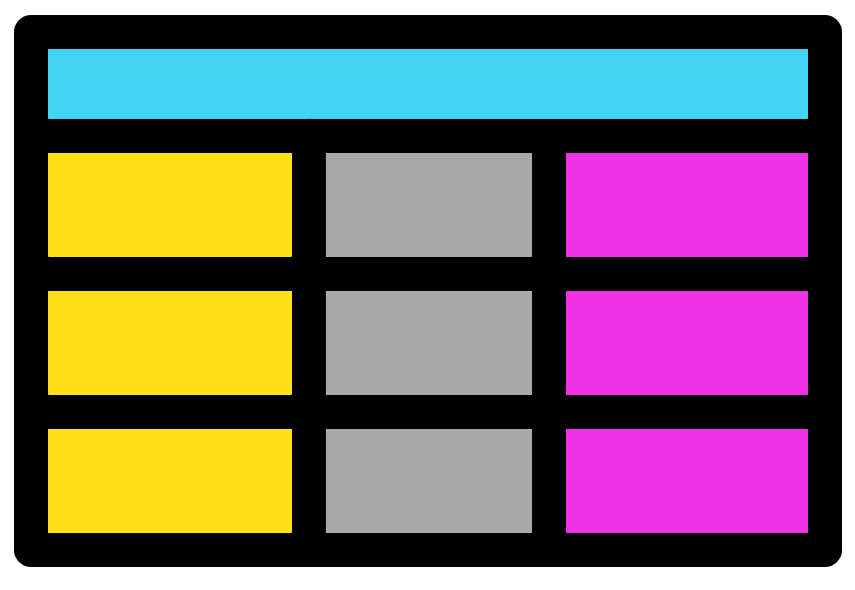
\includegraphics[width=0.2\linewidth]{figures/R_df} \end{center}

\section{Reading from a file}\label{reading-from-a-file}

\begin{center}
\includegraphics[width=0.2\linewidth]{figures/r_read} \end{center}

Last week we created \textbf{data frames} with R \textbf{functions}.
This was useful to help understand how \textbf{data frames} work in R.
However, in real life you will most likely not do this very often.
Instead you are more likely going to have data files you need to analyse
with R.

You can get your data into R by having R \textbf{read} your file.

The first task to carry out this week is to \textbf{read} in the file
``Liverpool\_beaches.csv''. Before \textbf{reading} in the file we can
check the contents of the file. This can be carried out by opening it
with notepad (or similar text tool) or viewing the file with RStudio.

To view the file with RStudio:

\begin{itemize}
\tightlist
\item
  Use the \textbf{Files pane} of the \textbf{MISC window} to navigate to
  the directory containing the file.
\item
  Click on the file name and then click ``View File''
\item
  This will open a tab in the \textbf{Source window} matching the file
  name
\end{itemize}

You will notice that the values are sperarated by commas as this is a
``comma seperated value'' (.csv) file. Additionally, this is the same
data as the ``beach\_df\_2'' \textbf{data frame} you created in last
week's exercises.

There are various \textbf{functions} to \textbf{read} in files into R.
My favourite that I find most consistent is `read.csv(). Use this
function to \textbf{read} in the file ``Liverpool\_beaches.csv'':

\begin{Shaded}
\begin{Highlighting}[]
\NormalTok{liv_beaches_df <-}\StringTok{ }\KeywordTok{read.csv}\NormalTok{(}\StringTok{"Liverpool_beaches.csv"}\NormalTok{)}
\end{Highlighting}
\end{Shaded}

Have a look at the newly created \textbf{data frame}. Is it how you
would like it?

The row names are empty and the beach names are in the first column. Let
us fix this and make it so the beach names are the row names. This can
be carried out by including the option \texttt{row.names\ =\ 1} to
specify the 1st column will be the row names:

\begin{Shaded}
\begin{Highlighting}[]
\NormalTok{liv_beaches_df <-}\StringTok{ }\KeywordTok{read.csv}\NormalTok{(}\StringTok{"Liverpool_beaches.csv"}\NormalTok{, }\DataTypeTok{row.names =} \DecValTok{1}\NormalTok{)}
\end{Highlighting}
\end{Shaded}

We know how to \textbf{read} in a csv file with \texttt{read.csv}, now
let us \textbf{read} in a tab seperated file with \texttt{read.csv}. As
before first look at the file contents before \textbf{reading} them in.
It contains the sales figures of fictional clothing stores through the
seasons.

Now use \texttt{read.csv()} to \textbf{read} in the file. We'll set
\texttt{row.names\ =\ 1} again but we will also include the option
\texttt{sep\ =\ "\textbackslash{}t"}. This option specifies the columns
are sperated (sep) by tabs (\texttt{"\textbackslash{}t"}).

\begin{Shaded}
\begin{Highlighting}[]
\NormalTok{clothing_df <-}\StringTok{ }\KeywordTok{read.csv}\NormalTok{(}\StringTok{"Clothing_stores.txt"}\NormalTok{, }\DataTypeTok{row.names =} \DecValTok{1}\NormalTok{, }\DataTypeTok{sep =} \StringTok{"}\CharTok{\textbackslash{}t}\StringTok{"}\NormalTok{)}
\end{Highlighting}
\end{Shaded}

Look at the resulting \textbf{data frame} and you will notice the column
names have been changed by R. This is annoying but thankfully there is
an easy fix. \textbf{Read} in the data again with the inclusion of the
parameter \texttt{check.names\ =\ FALSE}. This will stop the function
\texttt{read.csv()} from `checking' and `fixing' the column names. I
always use this option.

\begin{Shaded}
\begin{Highlighting}[]
\NormalTok{clothing_df <-}\StringTok{ }\KeywordTok{read.csv}\NormalTok{(}\StringTok{"Clothing_stores.txt"}\NormalTok{, }\DataTypeTok{row.names =} \DecValTok{1}\NormalTok{, }
                        \DataTypeTok{sep =} \StringTok{"}\CharTok{\textbackslash{}t}\StringTok{"}\NormalTok{, }\DataTypeTok{check.names =} \OtherTok{FALSE}\NormalTok{)}
\end{Highlighting}
\end{Shaded}

You may want to open excel files with R. Normally to do this I open the
file in excel and save it as a .csv or a tab seperated file and
\textbf{read} this into R. Alternatively there are R packages that can
directly \textbf{read} in excel files. If this is something you would
like to do you can look at the following package:

\url{https://readxl.tidyverse.org/}

An important note is that \textbf{reading} in a file into R will not
change the file. You are creating a new R \textbf{object}. Modifying
this \textbf{object} will not alter the original file. Later in the
materials we will look into how to create new files or overwrite files
by \textbf{writing}.

\section{Subsetting data}\label{subsetting-data}

\begin{center}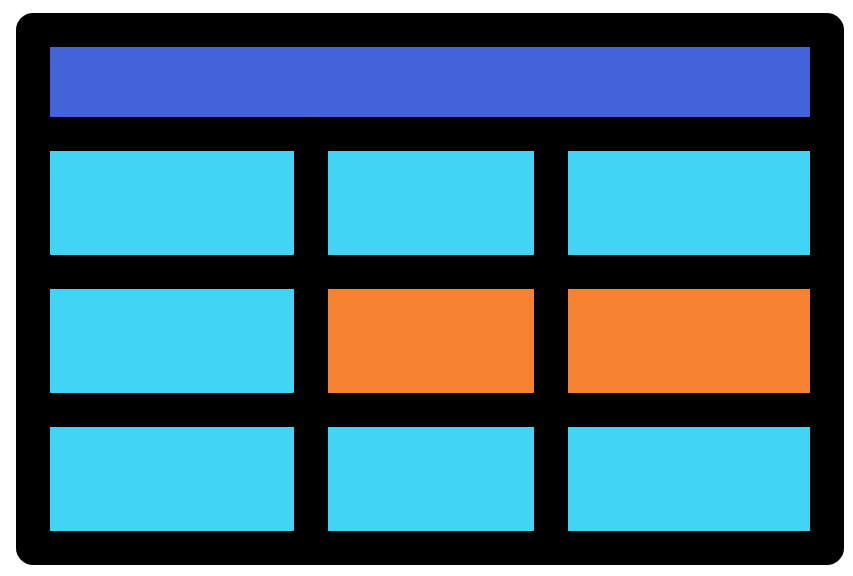
\includegraphics[width=0.2\linewidth]{figures/R_subset} \end{center}

R allows you to specify specific points in \textbf{R objects}. This is
one of the primary reasons R is so useful and flexible. With good use of
\textbf{assignment operators} this allows for the subsetting of
\textbf{variables}.

\subsection{Vectors}\label{vectors}

\begin{center}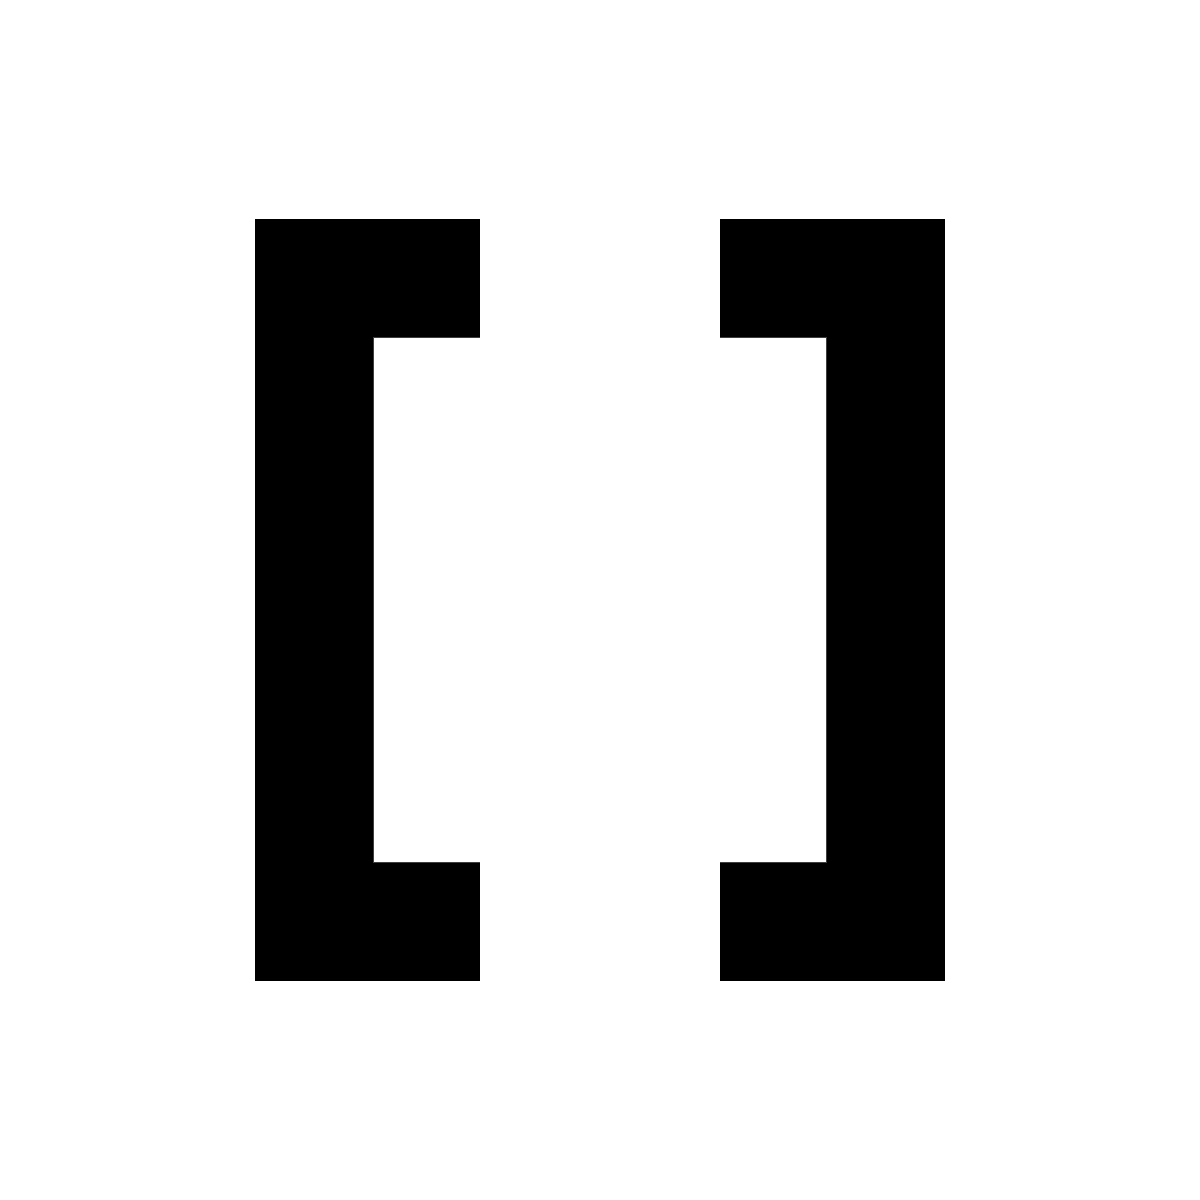
\includegraphics[width=0.2\linewidth]{figures/R_square_bracket} \end{center}

We will start with \textbf{vectors}. Before carrying out and subsetting
let us create some new \textbf{vectors}. We will use a new
\textbf{function} to create these, \texttt{seq()}.

\textbf{Tip}: Look at the resulting \textbf{vectors} and, use
\texttt{?seq()} or search online to understand the \texttt{seq()}
\textbf{function} better.

\begin{Shaded}
\begin{Highlighting}[]
\NormalTok{even_seq <-}\StringTok{ }\KeywordTok{seq}\NormalTok{(}\DataTypeTok{from =} \DecValTok{0}\NormalTok{, }\DataTypeTok{to =} \DecValTok{8}\NormalTok{, }\DataTypeTok{by =} \DecValTok{2}\NormalTok{)}
\NormalTok{odd_seq <-}\StringTok{ }\KeywordTok{seq}\NormalTok{(}\DataTypeTok{from =} \DecValTok{1}\NormalTok{, }\DataTypeTok{to =} \DecValTok{9}\NormalTok{, }\DataTypeTok{by =} \DecValTok{2}\NormalTok{)}
\NormalTok{long_seq <-}\StringTok{ }\KeywordTok{seq}\NormalTok{(}\DataTypeTok{from =} \DecValTok{10}\NormalTok{, }\DataTypeTok{to =} \DecValTok{300}\NormalTok{, }\DataTypeTok{by =} \DecValTok{10}\NormalTok{)}
\end{Highlighting}
\end{Shaded}

Grand! Now let us subset the \textbf{vectors} with square brackets
\texttt{{[}{]}}.

\textbf{Vectors} are one-dimensional, we therefore provide the square
brackets with one number or one range of numbers. The number/s we
provide in the square brackets are the index.

Try out indexxing/subsetting the \textbf{vectors}.

\begin{Shaded}
\begin{Highlighting}[]
\NormalTok{even_seq[}\DecValTok{2}\NormalTok{]}
\NormalTok{odd_seq[}\DecValTok{1}\NormalTok{]}
\NormalTok{long_seq[}\DecValTok{10}\NormalTok{]}
\NormalTok{even_seq[}\DecValTok{2}\OperatorTok{:}\DecValTok{3}\NormalTok{]}
\NormalTok{odd_seq[}\DecValTok{1}\OperatorTok{:}\DecValTok{4}\NormalTok{]}
\NormalTok{long_seq[}\DecValTok{21}\OperatorTok{:}\DecValTok{24}\NormalTok{]}
\NormalTok{long_seq[}\DecValTok{24}\OperatorTok{:}\DecValTok{21}\NormalTok{]}
\NormalTok{even_seq[}\KeywordTok{c}\NormalTok{(}\DecValTok{2}\NormalTok{,}\DecValTok{3}\NormalTok{)]}
\NormalTok{odd_seq[}\KeywordTok{c}\NormalTok{(}\DecValTok{1}\NormalTok{,}\DecValTok{3}\NormalTok{,}\DecValTok{2}\NormalTok{,}\DecValTok{5}\NormalTok{)]}
\NormalTok{long_seq[}\KeywordTok{c}\NormalTok{(}\DecValTok{1}\NormalTok{,}\DecValTok{21}\NormalTok{,}\DecValTok{21}\OperatorTok{:}\DecValTok{24}\NormalTok{,}\DecValTok{24}\OperatorTok{:}\DecValTok{21}\NormalTok{,}\DecValTok{1}\NormalTok{)]}
\CommentTok{#As long as the contents within the [] equal numbers they will work}
\NormalTok{even_seq[}\KeywordTok{seq}\NormalTok{(}\DataTypeTok{from =} \DecValTok{1}\NormalTok{, }\DataTypeTok{to =} \DecValTok{3}\NormalTok{, }\DataTypeTok{by =} \DecValTok{2}\NormalTok{)]}
\NormalTok{even_seq[}\KeywordTok{seq}\NormalTok{(}\DataTypeTok{from =} \DecValTok{0}\NormalTok{, }\DataTypeTok{to =} \DecValTok{5}\NormalTok{, }\DataTypeTok{by =} \DecValTok{3}\NormalTok{)]}
\NormalTok{long_seq[}\KeywordTok{seq}\NormalTok{(}\DataTypeTok{from =} \DecValTok{1}\NormalTok{, }\DataTypeTok{to =} \DecValTok{19}\NormalTok{, }\DataTypeTok{by =} \DecValTok{2}\NormalTok{)]}
\NormalTok{even_seq[}\DecValTok{1}\OperatorTok{*}\DecValTok{2}\NormalTok{]}
\NormalTok{odd_seq[}\DecValTok{2}\OperatorTok{/}\DecValTok{1}\NormalTok{]}
\NormalTok{long_seq[(}\DecValTok{1}\OperatorTok{:}\DecValTok{10}\NormalTok{)}\OperatorTok{*}\DecValTok{2}\NormalTok{]}
\end{Highlighting}
\end{Shaded}

The \textbf{vectors} even\_seq and odd\_seq have the indexes 1,2,3,4,
and 5 as they each contain 5 \textbf{scalars}. What if we try to use a
higher number to index than is avalable?

\begin{Shaded}
\begin{Highlighting}[]
\NormalTok{even_seq[}\DecValTok{6}\NormalTok{]}
\NormalTok{even_seq[}\KeywordTok{c}\NormalTok{(}\DecValTok{4}\NormalTok{,}\DecValTok{7}\NormalTok{)]}
\NormalTok{odd_seq[}\DecValTok{3}\OperatorTok{:}\DecValTok{9}\NormalTok{]}
\end{Highlighting}
\end{Shaded}

As you can see the above all work with no complaints. Any indexes that
are out of range will return a \texttt{NA} value. \texttt{NA} stands for
`Not Available'. We will not go into how \texttt{NA} works in R too
much. The most important thing to know about \texttt{NA} is that you
will most likely get \texttt{NA} if you use \textbf{operators} or
\textbf{functions} with \texttt{NA}. Below are a few examples:

\begin{Shaded}
\begin{Highlighting}[]
\CommentTok{#Will give NA}
\DecValTok{1} \OperatorTok{+}\StringTok{ }\OtherTok{NA}
\DecValTok{2} \OperatorTok{-}\StringTok{ }\OtherTok{NA}
\NormalTok{even_seq[}\DecValTok{2}\NormalTok{] }\OperatorTok{*}\StringTok{ }\OtherTok{NA}
\NormalTok{odd_seq[}\DecValTok{5}\NormalTok{] }\OperatorTok{/}\StringTok{ }\OtherTok{NA}
\CommentTok{#mean() function without NA}
\KeywordTok{mean}\NormalTok{(even_seq[}\DecValTok{2}\OperatorTok{:}\DecValTok{5}\NormalTok{])}
\CommentTok{#mean() function with NA}
\KeywordTok{mean}\NormalTok{(}\KeywordTok{c}\NormalTok{(}\DecValTok{1}\NormalTok{,}\DecValTok{2}\NormalTok{,}\DecValTok{3}\NormalTok{,}\DecValTok{4}\NormalTok{,}\DecValTok{5}\NormalTok{,}\OtherTok{NA}\NormalTok{))}
\KeywordTok{mean}\NormalTok{(even_seq[}\DecValTok{2}\OperatorTok{:}\DecValTok{7}\NormalTok{])}
\end{Highlighting}
\end{Shaded}

Above we subsetted \textbf{vectors} by specifying which indexes we want.
We can also specify which indexes we don't want:

\begin{Shaded}
\begin{Highlighting}[]
\NormalTok{even_seq[}\OperatorTok{-}\DecValTok{2}\NormalTok{]}
\NormalTok{odd_seq[}\OperatorTok{-}\DecValTok{3}\OperatorTok{:-}\DecValTok{5}\NormalTok{]}
\NormalTok{long_seq[}\KeywordTok{c}\NormalTok{(}\OperatorTok{-}\DecValTok{1}\NormalTok{,}\OperatorTok{-}\DecValTok{2}\NormalTok{,}\OperatorTok{-}\DecValTok{6}\NormalTok{)]}
\end{Highlighting}
\end{Shaded}

The \texttt{rep()} \textbf{function} will replicate a
\textbf{scalar/vector} a specified amount of times. We will use this
\textbf{function} to overwrite our previously created \textbf{variables}
with longer versions:

\begin{Shaded}
\begin{Highlighting}[]
\CommentTok{#Replicate vector even_seq 2 times}
\KeywordTok{rep}\NormalTok{(}\DataTypeTok{x =}\NormalTok{ even_seq, }\DecValTok{2}\NormalTok{)}
\CommentTok{#Replicate vector even_seq 4 times and then assign even_seq as the newly created vector}
\NormalTok{even_seq <-}\StringTok{ }\KeywordTok{rep}\NormalTok{(}\DataTypeTok{x =}\NormalTok{ even_seq, }\DecValTok{4}\NormalTok{)}
\CommentTok{#More examples}
\NormalTok{odd_seq <-}\StringTok{ }\KeywordTok{rep}\NormalTok{(}\DataTypeTok{x =}\NormalTok{ odd_seq, }\DecValTok{4}\NormalTok{)}
\NormalTok{long_seq <-}\StringTok{ }\KeywordTok{rep}\NormalTok{(}\DataTypeTok{x =}\NormalTok{ long_seq, }\DecValTok{3}\NormalTok{)}
\end{Highlighting}
\end{Shaded}

\textbf{Logical} \textbf{operators} can be used as indexes to subset
\textbf{vectors}. Having a logical expression (i.e.~1 \textgreater{} 2)
as the index will cause all TRUE positions to be included and all FALSE
positions to be excluded.

\textbf{Tip}: If it is difficult to deduce what the below commands are
doing you can run the part in the square brackets by itself. Remember if
you highlight code in the \textbf{script editor} it will only run that
part, including parts of script in the same line.

\begin{Shaded}
\begin{Highlighting}[]
\NormalTok{even_seq }\OperatorTok{>}\StringTok{ }\DecValTok{3}
\NormalTok{even_seq[even_seq  }\OperatorTok{>}\StringTok{ }\DecValTok{2}\NormalTok{]}
\NormalTok{odd_seq[odd_seq }\OperatorTok{<=}\StringTok{ }\DecValTok{1}\NormalTok{ ]}
\NormalTok{long_seq <-}\StringTok{ }\NormalTok{long_seq[long_seq }\OperatorTok{<}\StringTok{ }\DecValTok{50}\NormalTok{]}
\end{Highlighting}
\end{Shaded}

We will quickly look at a new \textbf{operator}, \texttt{\%\%}. This is
the modulus \textbf{operator}, it divides two numbers and gives the
remainder of the division.

With the modulus \textbf{operator}, logical expressions, and subsetting
we can extract even or odd numbers from a \textbf{vector}:

\begin{Shaded}
\begin{Highlighting}[]
\CommentTok{#First some basic modulus examples}
\DecValTok{2}\OperatorTok\DecValTok{2}
\DecValTok{3}\OperatorTok\DecValTok{2}
\CommentTok{#Create a vector with numbers 0 to 9}
\NormalTok{single_digit_vec <-}\StringTok{ }\DecValTok{0}\OperatorTok{:}\DecValTok{9}
\CommentTok{#Extract even numbers then odd numbers from the vector}
\CommentTok{#We carry this out by determining if numbers are divisible by 2 or not}
\NormalTok{even_seq <-}\StringTok{ }\NormalTok{single_digit_vec[(single_digit_vec }\OperatorTok\StringTok{ }\DecValTok{2}\NormalTok{) }\OperatorTok{==}\StringTok{ }\DecValTok{0}\NormalTok{ ]}
\NormalTok{odd_seq <-}\StringTok{ }\NormalTok{single_digit_vec[(single_digit_vec }\OperatorTok\StringTok{ }\DecValTok{2}\NormalTok{) }\OperatorTok{!=}\StringTok{ }\DecValTok{0}\NormalTok{]}
\CommentTok{#We can determine which numbers in a vector are divisible by any specific number}
\CommentTok{#Divisible by 3}
\CommentTok{#remember variable names cannot start with numbers}
\NormalTok{divis_3_vec <-}\StringTok{ }\NormalTok{single_digit_vec[(single_digit_vec }\OperatorTok\StringTok{ }\DecValTok{3}\NormalTok{) }\OperatorTok{==}\StringTok{ }\DecValTok{0}\NormalTok{]}
\CommentTok{#Divisible by 7}
\NormalTok{divis_7_vec <-}\StringTok{ }\NormalTok{single_digit_vec[(single_digit_vec }\OperatorTok\StringTok{ }\DecValTok{7}\NormalTok{) }\OperatorTok{==}\StringTok{ }\DecValTok{0}\NormalTok{]}
\CommentTok{#Try out other numbers!}
\end{Highlighting}
\end{Shaded}

\subsection{Data frames}\label{data-frames}

\begin{center}
\includegraphics[width=0.2\linewidth]{figures/envelope} \end{center}

\textbf{Data frames} can be subset similar to \textbf{vectors}. As with
\textbf{vectors} you can use \texttt{{[}{]}}. Additonally \texttt{\$}
can be used to subset \textbf{data frames}.

Square brackets must be provided indexes for rows and for columns. The
structure for this is \texttt{df{[}row,column{]}}. It is very useful to
remember that R always wants rows first then columns second.

To practice subsetting \textbf{data frames} with square brackets we will
\textbf{read} in a new file called ``Census\_2011\_L\_postcodes.csv''.
This contains UK 2011 census information on total residents for
postcodes that start with the letter L. Data can be found:

\url{https://www.nomisweb.co.uk/census/2011/postcode_headcounts_and_household_estimates}

\begin{Shaded}
\begin{Highlighting}[]
\NormalTok{L_2011_census_df <-}\StringTok{ }\KeywordTok{read.csv}\NormalTok{(}\StringTok{"Census_2011_L_postcodes_counts.csv"}\NormalTok{, }\DataTypeTok{check.names =} \OtherTok{FALSE}\NormalTok{,}
                             \DataTypeTok{row.names =} \DecValTok{1}\NormalTok{)}
\end{Highlighting}
\end{Shaded}

Now for some subset commands:

\begin{Shaded}
\begin{Highlighting}[]
\CommentTok{#Scalar from the 1st row and 1st column}
\NormalTok{L_2011_census_df[}\DecValTok{1}\NormalTok{,}\DecValTok{1}\NormalTok{]}
\CommentTok{#Row names and column names can be used for indexxing}
\CommentTok{#Scalar from the row called L10 1LD: E00033706 and the column called Postcode}
\NormalTok{L_2011_census_df[}\StringTok{"L10 1LD"}\NormalTok{,}\StringTok{"Area"}\NormalTok{]}
\CommentTok{#More examples}
\NormalTok{L_2011_census_df[}\DecValTok{1}\OperatorTok{:}\DecValTok{10}\NormalTok{,}\DecValTok{2}\NormalTok{]}
\NormalTok{L_2011_census_df[}\DecValTok{1}\OperatorTok{:}\DecValTok{10}\NormalTok{,}\StringTok{"District"}\NormalTok{]}
\NormalTok{L_2011_census_df[}\DecValTok{3}\NormalTok{,}\DecValTok{2}\OperatorTok{:}\DecValTok{4}\NormalTok{]}
\NormalTok{L_2011_census_df[}\StringTok{"L10 1LD"}\NormalTok{,}\DecValTok{2}\NormalTok{]}
\NormalTok{L_2011_census_df[}\DecValTok{1}\OperatorTok{:}\DecValTok{10}\NormalTok{,}\StringTok{"Total"}\NormalTok{]}
\NormalTok{L_2011_census_df[}\KeywordTok{c}\NormalTok{(}\DecValTok{1}\NormalTok{,}\DecValTok{3}\NormalTok{,}\DecValTok{5}\NormalTok{,}\DecValTok{6}\NormalTok{),}\KeywordTok{c}\NormalTok{(}\StringTok{"Total"}\NormalTok{,}\StringTok{"Occupied_Households"}\NormalTok{)]}
\end{Highlighting}
\end{Shaded}

Depending on how you subset a \textbf{data frame} you may get a
\textbf{scalar}, \textbf{vector}, or \textbf{data frame}. Below
describes which you will get based on the subsetting.

\begin{itemize}
\tightlist
\item
  \textbf{Scalar}:

  \begin{itemize}
  \tightlist
  \item
    Indexxing to get a single value by choosing one row and one column.
  \item
    E.g. \texttt{L\_2011\_census\_df{[}1,1{]}}
  \end{itemize}
\item
  \textbf{Vector}:

  \begin{itemize}
  \tightlist
  \item
    Indexxing so you get multiple values from one column. This occurs as
    each column is in essence a \textbf{vector}.
  \item
    E.g. \texttt{L\_2011\_census\_df{[}1:10,2{]}}
  \end{itemize}
\item
  \textbf{Data frame}:

  \begin{itemize}
  \tightlist
  \item
    Indexxing so you get multiple values from a row or multiple rows.
    Subsetting a \textbf{data frame} like this provides you a
    \textbf{data frame}.
  \item
    E.g. \texttt{L\_2011\_census\_df{[}3,2:4{]}} or
    \texttt{L\_2011\_census\_df{[}3:4,2:4{]}}
  \end{itemize}
\end{itemize}

A quick \textbf{function} to subset a \textbf{data frame} is
\texttt{head()}. By default it will return the first 6 rows.

\begin{Shaded}
\begin{Highlighting}[]
\CommentTok{#Return first 6 rows}
\KeywordTok{head}\NormalTok{(L_2011_census_df)}
\CommentTok{#Return first 10 rows}
\KeywordTok{head}\NormalTok{(L_2011_census_df, }\DecValTok{10}\NormalTok{)}
\end{Highlighting}
\end{Shaded}

The \textbf{data frame} is quite large. We will therefore use the
\texttt{head()} \textbf{function} and the \textbf{assignment operator}
to make the \textbf{data frame} smaller for further examples.

\begin{Shaded}
\begin{Highlighting}[]
\NormalTok{L_2011_census_df <-}\StringTok{ }\KeywordTok{head}\NormalTok{(L_2011_census_df, }\DecValTok{20}\NormalTok{)}
\end{Highlighting}
\end{Shaded}

To return all the rows of the specified columns you can leave the part
before the comma empty. Similarly you can leave the part after the comma
empty to return all of the columns of the specified rows. Leave both
sides empty and you will get the entire \textbf{data frame}.

\begin{Shaded}
\begin{Highlighting}[]
\NormalTok{L_2011_census_df[,]}
\NormalTok{L_2011_census_df[,}\DecValTok{2}\NormalTok{]}
\NormalTok{L_2011_census_df[}\DecValTok{3}\NormalTok{,]}
\NormalTok{L_2011_census_df[,}\StringTok{"District"}\NormalTok{]}
\NormalTok{L_2011_census_df[}\DecValTok{2}\OperatorTok{:}\DecValTok{4}\NormalTok{,]}
\end{Highlighting}
\end{Shaded}

The sign \texttt{\$} allows you to indicate which column you would like
from the \textbf{data frame}. This is done like so:

\begin{Shaded}
\begin{Highlighting}[]
\NormalTok{L_2011_census_df}\OperatorTok{$}\NormalTok{Area}
\NormalTok{L_2011_census_df}\OperatorTok{$}\NormalTok{District}
\NormalTok{L_2011_census_df}\OperatorTok{$}\NormalTok{Total}
\end{Highlighting}
\end{Shaded}

You will notice that the above commands return \textbf{vectors}. We can
therefore subset these \textbf{vectors} with \texttt{{[}{]}}:

\begin{Shaded}
\begin{Highlighting}[]
\NormalTok{L_2011_census_df}\OperatorTok{$}\NormalTok{Area[}\DecValTok{2}\NormalTok{]}
\NormalTok{L_2011_census_df}\OperatorTok{$}\NormalTok{District[}\DecValTok{2}\NormalTok{]}
\NormalTok{L_2011_census_df}\OperatorTok{$}\NormalTok{Total[}\DecValTok{4}\OperatorTok{:}\DecValTok{7}\NormalTok{]}
\end{Highlighting}
\end{Shaded}

Below are a selection of useful \textbf{functions} that can be used on
\textbf{vectors}.

\begin{Shaded}
\begin{Highlighting}[]
\CommentTok{#Sum the values of a numeric vector}
\KeywordTok{sum}\NormalTok{(L_2011_census_df}\OperatorTok{$}\NormalTok{Total)}
\CommentTok{#Mean of the values of a numeric vector}
\KeywordTok{mean}\NormalTok{(L_2011_census_df}\OperatorTok{$}\NormalTok{Total)}
\end{Highlighting}
\end{Shaded}

The above \textbf{functions} are useful but limiting if you are working
with \textbf{data frames}. Thankfully there are also many
\textbf{functions} used specifically for \textbf{data frames} (they can
also be used for matrices).

\begin{Shaded}
\begin{Highlighting}[]
\CommentTok{#Sum numeric columns}
\KeywordTok{colSums}\NormalTok{(L_2011_census_df[,}\DecValTok{3}\OperatorTok{:}\DecValTok{6}\NormalTok{])}
\CommentTok{#Sum numeric rows}
\KeywordTok{rowSums}\NormalTok{(L_2011_census_df[,}\DecValTok{4}\OperatorTok{:}\DecValTok{5}\NormalTok{])}
\CommentTok{#Mean of numeric columns}
\KeywordTok{colMeans}\NormalTok{(L_2011_census_df[,}\DecValTok{3}\OperatorTok{:}\DecValTok{6}\NormalTok{])}
\CommentTok{#Mean of numeric rows}
\KeywordTok{rowMeans}\NormalTok{(L_2011_census_df[,}\DecValTok{4}\OperatorTok{:}\DecValTok{5}\NormalTok{])}
\CommentTok{#Summary information for each column}
\CommentTok{#This works for string and numeric columns with different outputs}
\KeywordTok{summary}\NormalTok{(L_2011_census_df)}
\end{Highlighting}
\end{Shaded}

Try out some of the above commands with the entire \textbf{data frame}.
Do they give an error? Is so, why?

Before we learn how to \textbf{write} data to a file I will introduce
one more \textbf{data frame} associated \textbf{function}. \texttt{t()}
which stands for transpose:

\begin{Shaded}
\begin{Highlighting}[]
\NormalTok{L_2011_census_df[}\DecValTok{3}\OperatorTok{:}\DecValTok{5}\NormalTok{]}
\KeywordTok{t}\NormalTok{(L_2011_census_df[,}\DecValTok{3}\OperatorTok{:}\DecValTok{5}\NormalTok{])}
\KeywordTok{summary}\NormalTok{(}\KeywordTok{t}\NormalTok{(L_2011_census_df[,}\DecValTok{3}\OperatorTok{:}\DecValTok{5}\NormalTok{]))}
\end{Highlighting}
\end{Shaded}

Try the above commands without subsetting the \textbf{data frame}. What
is happening and why?

\section{Writing to a file}\label{writing-to-a-file}

\begin{center}
\includegraphics[width=0.2\linewidth]{figures/R_writing} \end{center}

Before we \textbf{write} data to a file we will create a new
\textbf{data frame} from ``L\_2011\_census\_df''.

First I like to create a new \textbf{variable} from our old
\textbf{variable} if there are many steps. This means if we make a
mistake we can go back and recreate the new \textbf{variable}.

\begin{Shaded}
\begin{Highlighting}[]
\NormalTok{L_2011_census_t_df <-}\StringTok{ }\NormalTok{L_2011_census_df}
\end{Highlighting}
\end{Shaded}

Next step we will create a new column called
``Average\_per\_occupied\_households''.

\textbf{NOTE}: I am including many ways to subset columns as reminders.
Normally I wouldn't have so many different ways in one command.

\textbf{NOTE}: We are using ``\_" instead of spaces as R doesn't
particularly like spaces in column names. We will see how to use spaces
later.

\begin{Shaded}
\begin{Highlighting}[]
\NormalTok{L_2011_census_t_df}\OperatorTok{$}\NormalTok{Average_per_occupied_households <-}\StringTok{ }
\StringTok{  }\NormalTok{L_2011_census_t_df[,}\DecValTok{3}\NormalTok{] }\OperatorTok{/}\StringTok{ }\NormalTok{L_2011_census_t_df[,}\StringTok{"Occupied_Households"}\NormalTok{]}
\end{Highlighting}
\end{Shaded}

Have a look at the current \textbf{data frame}. You may notice an
\texttt{Inf} value. This appears as when you divide a number by 0 in R
you will get \texttt{Inf}. I am not sure how a Post code has 174
residents and 0 Occupied households but it doesn't matter for us.

The final step before writing is to transpose the \textbf{data frame}
leaving out the Area and District columns:

\begin{Shaded}
\begin{Highlighting}[]
\CommentTok{#Transpose dataframe}
\NormalTok{L_2011_census_t_df <-}\StringTok{ }\KeywordTok{t}\NormalTok{(L_2011_census_t_df[,}\DecValTok{3}\OperatorTok{:}\DecValTok{7}\NormalTok{])}
\CommentTok{#Check structure}
\KeywordTok{str}\NormalTok{(L_2011_census_t_df)}
\CommentTok{#It is not a dataframe}
\CommentTok{#Let us therefore convert it to a data frame}
\NormalTok{L_2011_census_t_df <-}\StringTok{ }\KeywordTok{as.data.frame}\NormalTok{(L_2011_census_t_df)}
\CommentTok{#Structure check}
\KeywordTok{str}\NormalTok{(L_2011_census_t_df)}
\end{Highlighting}
\end{Shaded}

After all that let us \textbf{write} the \textbf{data frame} to a file
called ``Census\_info\_2011.csv''. When \textbf{reading} from a file a
prefer \texttt{read.csv()}, however when writing to a file I prefer
\texttt{write.table()}. With this \textbf{function} we will include the
option \texttt{sep=","} to have commas as the column seperators. We will
also include the option \texttt{col.names=NA} to create an empty space
above the row names. If this was not included then the first column name
would be above the row names.

\begin{Shaded}
\begin{Highlighting}[]
\KeywordTok{write.table}\NormalTok{(L_2011_census_t_df, }\DataTypeTok{file =} \StringTok{"Census_info_2011.csv"}\NormalTok{, }\DataTypeTok{sep =} \StringTok{","}\NormalTok{, }\DataTypeTok{col.names=}\OtherTok{NA}\NormalTok{)}
\end{Highlighting}
\end{Shaded}

Have a look at the file contents with RStudio.

Let us do it one more time with the clothing store info. First let us
\textbf{read} in the file again in case you do not have it. Then we will
create a total sales column and finally transpose the \textbf{data
frame}:

\begin{Shaded}
\begin{Highlighting}[]
\CommentTok{#Read in}
\NormalTok{clothing_df <-}\StringTok{ }\KeywordTok{read.csv}\NormalTok{(}\StringTok{"Clothing_stores.txt"}\NormalTok{, }\DataTypeTok{row.names =} \DecValTok{1}\NormalTok{, }
                        \DataTypeTok{sep =} \StringTok{"}\CharTok{\textbackslash{}t}\StringTok{"}\NormalTok{, }\DataTypeTok{check.names =} \OtherTok{FALSE}\NormalTok{)}
\CommentTok{#Create total column}
\CommentTok{#We are referring to a column name with spaces}
\CommentTok{#Therefore we must surround the name with `}
\CommentTok{#The button for ` is left of the 1 key and below the esc key}
\NormalTok{clothing_df}\OperatorTok{$}\StringTok{`}\DataTypeTok{Total sales}\StringTok{`}\NormalTok{ <-}\StringTok{ }\KeywordTok{rowSums}\NormalTok{(clothing_df)}
\CommentTok{#Transpose ensuring output is a data frame}
\NormalTok{clothing_t_df <-}\StringTok{ }\KeywordTok{as.data.frame}\NormalTok{(}\KeywordTok{t}\NormalTok{(clothing_df))}
\end{Highlighting}
\end{Shaded}

\textbf{Write} the \textbf{data frame} to a tab delimited file (.tsv).
This time we will make it so the row and column names are not surrounded
by quotes:

\begin{Shaded}
\begin{Highlighting}[]
\KeywordTok{write.table}\NormalTok{(clothing_t_df, }
            \StringTok{"Clothing_stores_transposed.tsv"}\NormalTok{, }
            \DataTypeTok{sep =} \StringTok{"}\CharTok{\textbackslash{}t}\StringTok{"}\NormalTok{,  }
            \DataTypeTok{col.names=}\OtherTok{NA}\NormalTok{, }
            \DataTypeTok{quote =} \OtherTok{FALSE}\NormalTok{)}
\end{Highlighting}
\end{Shaded}

With the fundamentals of \textbf{reading}, subsetting \textbf{data
frames}, and writing covered it is time to carry out some exercises.

\chapter{Week 3 exercises}\label{week-3-exercises}

This exercise will look at two files. You will be assigned tasks
requiring you to \textbf{read} and \textbf{write} files as well as index
\textbf{data frames}

\section{Bats}\label{bats}

\begin{center}
\includegraphics[width=0.2\linewidth]{figures/bat} \end{center}

First we will look at the file ``bat\_roosts.csv''. This contains
information on the max number of roosts for different Bat species in
different UK regions.

The data is from: ``Bat Conservation Trust 2020. Roost Count peak counts
summary data. Available from
\url{https://www.bats.org.uk/our-work/national-bat-monitoring-programme/reports/nbmp-annual-report}''

For this file carry out the below tasks:

\begin{enumerate}
\def\labelenumi{\arabic{enumi}.}
\tightlist
\item
  \textbf{Read} in the file ``bat\_roosts.csv'' as a \textbf{data frame}
  \textbf{variable} called ``bat\_df''. Ensure the row names contain the
  Regions (Channel Islands, East Midlands, etc.)
\item
  Inspect the \textbf{variable} and ensure there are only numerics
  within the \textbf{data frame} with all strings only being in column
  and row names.
\item
  Add a row to ``bat\_df'' called ``UK'' that contains the totals for
  each Species.
\item
  Add a column to ``bat\_df'' called ``All\_Bat\_Species'' that contains
  the totals for each Region.
\item
  Create a transposed \textbf{data frame} of ``bat\_df'' called
  ``bat\_t\_df''.
\item
  \textbf{Write} the \textbf{data frame} ``bat\_t\_df'' to a comma
  seperated file called ``bat\_roosts\_t.csv''. Ensure there are no
  quotes surrounding the row or column names.
\end{enumerate}

Now that you have carried that out, can you answer the following
questions?

\begin{enumerate}
\def\labelenumi{\arabic{enumi}.}
\tightlist
\item
  Which region has no roosts?
\item
  Which Bat species has the highest number of roosts across the UK?
\item
  Which Bat species has the lowest number of roosts across the UK?
\end{enumerate}

\section{UK retail}\label{uk-retail}

\begin{center}
\includegraphics[width=0.2\linewidth]{figures/UKPounds} \end{center}

Next we have a file (``UK\_retail.txt'') containing UK retail
information for each month from September 2017 to September 2020. The
values are seasonally adjusted volume sales. The data comes from:
\url{https://www.ons.gov.uk/businessindustryandtrade/retailindustry/bulletins/retailsales/september2020}.

Carry out the below tasks:

\begin{enumerate}
\def\labelenumi{\arabic{enumi}.}
\tightlist
\item
  \textbf{Read} in the file ``UK\_retail.txt'' as a \textbf{data frame}
  \textbf{variable} called ``uk\_retail\_df''. Ensure the row names
  contain the YearMonth info (2017SEP, 2017OCT, etc.).
\item
  Create a \textbf{data frame} called ``retail\_2020\_df'' containing
  the rows for 2020 from ``uk\_retail\_df''.
\item
  For each month in 2020 print out the phrase ``The Food retail index
  for \textless{}YearMonth\textgreater{} was
  \textless{}Food\textgreater{}''. For example the first phrase will be
  ``The Food retail index for 2020JAN was 101.9''. This can be done with
  one line of code using the \texttt{paste()} function.
\item
  Make a total row and an average (mean) row for ``retail\_2020\_df''.
  Ensure you are not including the total in the mean.
\item
  Finally write out the \textbf{data frame} ``retail\_2020\_df'' as a
  tab seperated file called ``UK\_retail\_2020.tsv''.
\end{enumerate}

Now that you have carried that out, can you answer the following
questions?

\begin{enumerate}
\def\labelenumi{\arabic{enumi}.}
\tightlist
\item
  Which retail sectors have a lower average than their February 2020
  value?
\item
  Which retail sector was the highest for 2020?
\item
  Which sector was the most stable?
\end{enumerate}

Great! Have a look at the solution, ask any questions you would like,
then that is the end of this week.

\chapter{Week 3 exercise solutions}\label{week-3-exercise-solutions}

Before looking at these solutions keep in mind that there are many
different ways to do the same thing in R. Therefore if your scripts are
different than the ones below it does not mean they are wrong. As long
as they produce the intended output they are correct.

\section{Bats solution}\label{bats-solution}

\begin{center}
\includegraphics[width=0.2\linewidth]{figures/bat} \end{center}

Read in the file as a \textbf{data frame}:

\begin{Shaded}
\begin{Highlighting}[]
\NormalTok{bat_df <-}\StringTok{ }\KeywordTok{read.csv}\NormalTok{(}\StringTok{"bat_roosts.csv"}\NormalTok{, }\DataTypeTok{row.names =} \DecValTok{1}\NormalTok{, }\DataTypeTok{check.names =} \OtherTok{FALSE}\NormalTok{)}
\end{Highlighting}
\end{Shaded}

Add a row with column totals:

\begin{Shaded}
\begin{Highlighting}[]
\NormalTok{bat_df[}\StringTok{"UK"}\NormalTok{,] <-}\StringTok{ }\KeywordTok{colSums}\NormalTok{(bat_df) }
\end{Highlighting}
\end{Shaded}

Add a column with row totals:

\begin{Shaded}
\begin{Highlighting}[]
\NormalTok{bat_df}\OperatorTok{$}\NormalTok{All_Bat_Species <-}\StringTok{ }\KeywordTok{rowSums}\NormalTok{(bat_df) }
\end{Highlighting}
\end{Shaded}

Create transposed \textbf{data frame}:

\begin{Shaded}
\begin{Highlighting}[]
\NormalTok{bat_t_df <-}\StringTok{ }\KeywordTok{as.data.frame}\NormalTok{(}\KeywordTok{t}\NormalTok{(bat_df)) }
\end{Highlighting}
\end{Shaded}

\textbf{Write} file:

\begin{Shaded}
\begin{Highlighting}[]
\KeywordTok{write.table}\NormalTok{(bat_t_df, }\DataTypeTok{file =} \StringTok{"bat_roosts_t.csv"}\NormalTok{, }\DataTypeTok{sep =} \StringTok{","}\NormalTok{, }\DataTypeTok{quote =} \OtherTok{FALSE}\NormalTok{, }\DataTypeTok{col.names =} \OtherTok{NA}\NormalTok{)}
\end{Highlighting}
\end{Shaded}

\section{UK retail solution}\label{uk-retail-solution}

\begin{center}
\includegraphics[width=0.2\linewidth]{figures/UKPounds} \end{center}

Read in file:

\begin{Shaded}
\begin{Highlighting}[]
\NormalTok{retail_df <-}\StringTok{ }\KeywordTok{read.csv}\NormalTok{(}\StringTok{"UK_retail.txt"}\NormalTok{, }\DataTypeTok{sep =} \StringTok{"}\CharTok{\textbackslash{}t}\StringTok{"}\NormalTok{, }\DataTypeTok{row.names =} \DecValTok{1}\NormalTok{, }\DataTypeTok{check.names =} \OtherTok{FALSE}\NormalTok{)}
\end{Highlighting}
\end{Shaded}

Create 2020 \textbf{data frame}: Read in file:

\begin{Shaded}
\begin{Highlighting}[]
\CommentTok{#Can index to get the desired columns}
\NormalTok{retail_2020_df <-}\StringTok{ }\NormalTok{retail_df[}\DecValTok{29}\OperatorTok{:}\DecValTok{37}\NormalTok{,]}
\CommentTok{#Alternatively the tail() function can be used}
\CommentTok{#It is like head() but will get lowest rows}
\NormalTok{retail_2020_df <-}\StringTok{ }\KeywordTok{tail}\NormalTok{(retail_df, }\DataTypeTok{n =} \DecValTok{9}\NormalTok{)}
\end{Highlighting}
\end{Shaded}

Print food index phrases

\begin{Shaded}
\begin{Highlighting}[]
\KeywordTok{paste}\NormalTok{(}\StringTok{"The Food retail index for"}\NormalTok{, }\KeywordTok{row.names}\NormalTok{(retail_2020_df),}
      \StringTok{"was"}\NormalTok{, retail_2020_df}\OperatorTok{$}\NormalTok{Food, }
      \DataTypeTok{sep =} \StringTok{" "}\NormalTok{)}
\end{Highlighting}
\end{Shaded}

Total and mean rows

\begin{Shaded}
\begin{Highlighting}[]
\NormalTok{retail_2020_df[}\StringTok{"Total"}\NormalTok{,] <-}\StringTok{ }\KeywordTok{colSums}\NormalTok{(retail_2020_df)}
\NormalTok{retail_2020_df[}\StringTok{"Average"}\NormalTok{,] <-}\StringTok{ }\KeywordTok{colMeans}\NormalTok{(}\KeywordTok{head}\NormalTok{(retail_2020_df, }\DataTypeTok{n =} \DecValTok{9}\NormalTok{))}
\end{Highlighting}
\end{Shaded}

Write out file:

\begin{Shaded}
\begin{Highlighting}[]
\KeywordTok{write.table}\NormalTok{(retail_2020_df, }\StringTok{"UK_retail_2020.tsv"}\NormalTok{, }
            \DataTypeTok{sep =} \StringTok{"}\CharTok{\textbackslash{}t}\StringTok{"}\NormalTok{, }\DataTypeTok{col.names =} \OtherTok{NA}\NormalTok{, }\DataTypeTok{quote =} \OtherTok{FALSE}\NormalTok{)}
\end{Highlighting}
\end{Shaded}

\chapter{Week 4 - Handy tips \&
tricks}\label{week-4---handy-tips-tricks}

\begin{center}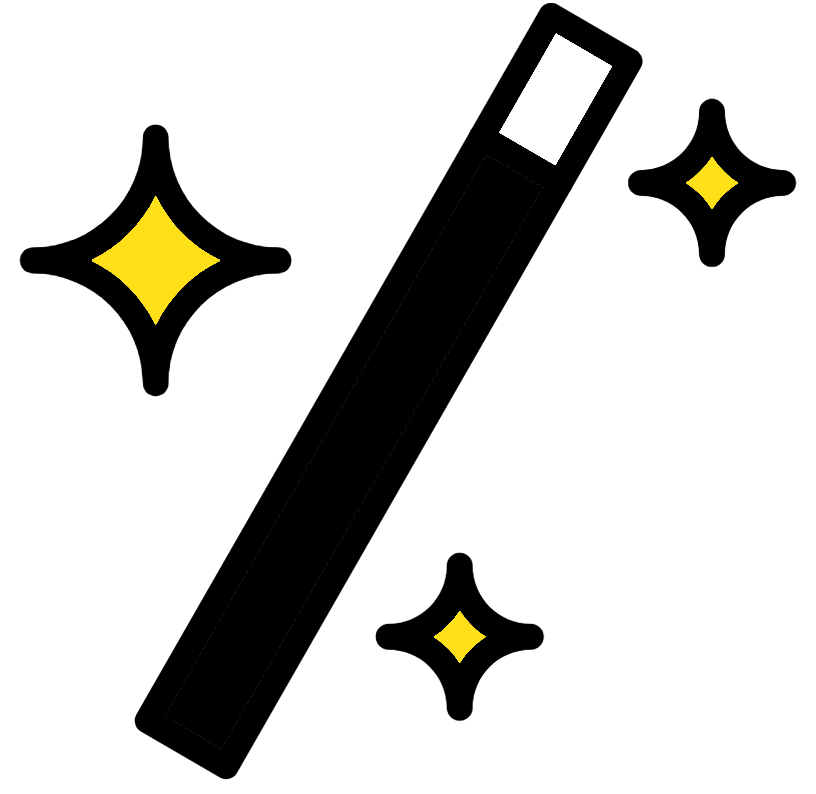
\includegraphics[width=0.2\linewidth]{figures/magic} \end{center}

Welcome to week 4! This week will include coding to reinforce what you
have learnt up to this point. There will also be plenty of new handy
\textbf{functions} and some more concepts to learn.

For this week create a script called ``Week3\_practice.R''. Remember to
use annotations (\texttt{\#}) and code sections (\texttt{\#\#\#\#})!

However, I'll first introduce you to some R conventions and then some
useful abilities of RStudio.

\section{R conventions}\label{r-conventions}

\begin{center}
\includegraphics[width=0.2\linewidth]{figures/rules} \end{center}

R conventions are style guides. You do not need to follow them but they
are intended to help make code easier to read. There are lots of
different suggestions for different parts of R code. Here we will only
look at conventions for \textbf{object/variable names} and wide vs long
code formatting.

\subsection{Variable names}\label{variable-names}

\textbf{Variable names} have certain rules that must be followed. We
covered these in week 1 but below is a reminder:

\begin{itemize}
\tightlist
\item
  Must start with a letter.
\item
  Cannot contain spaces.
\item
  Cannot start with a number.
\item
  Cannot share the same name as a command or function in R.
\item
  They are case sensitive. The \textbf{variable} name \texttt{BB} is
  differnet to the \textbf{variable} name \texttt{bb} which is differnet
  again to \texttt{bB}.
\end{itemize}

On top of these rules there are a few naming styles that are
recommended. It is very good to choose one naming style and stick with
it always. Below are three commonly used naming conventions for R. Look
through them and choose your favourite to use.

\subsubsection{Snake case}\label{snake-case}

\begin{center}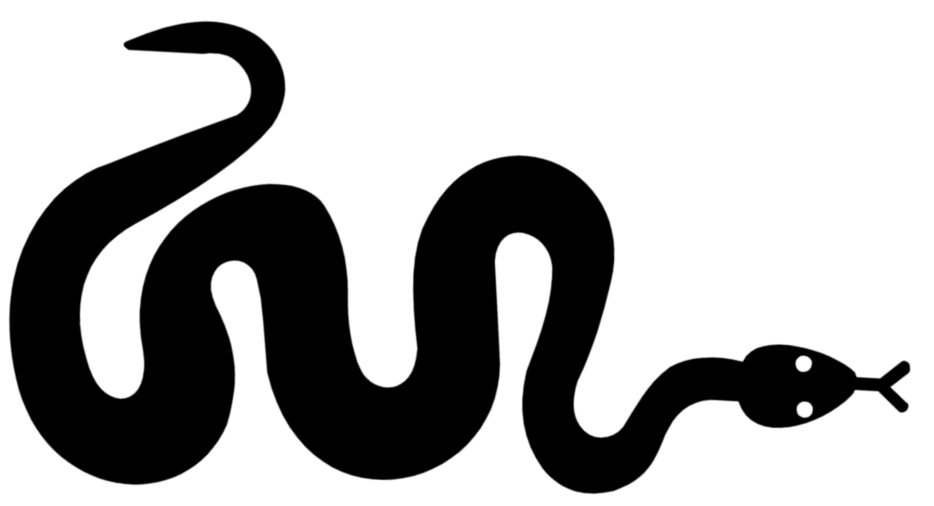
\includegraphics[width=0.2\linewidth]{figures/snake_case} \end{center}

Snake case is my preferred naming convention due to my background. It
consists of using lower case letters with underscores (\texttt{\_})
between words. Numbers can also be used. Below are some examples of
names in snake case.

\begin{Shaded}
\begin{Highlighting}[]
\NormalTok{one}
\NormalTok{two_df}
\NormalTok{two_2_df}
\NormalTok{three_four_five}
\NormalTok{three_four_five_2_vec}
\NormalTok{this_is_snake_case}
\end{Highlighting}
\end{Shaded}

\subsubsection{Period separated}\label{period-separated}

\begin{center}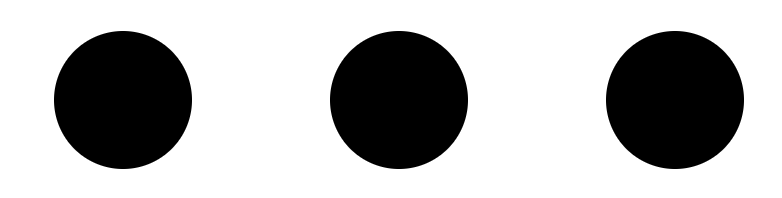
\includegraphics[width=0.2\linewidth]{figures/period_separated} \end{center}

Period seperated is almost identical to snake case. Just swap the
underscores (\texttt{\_}) with periods (\texttt{.}). Below are some
examples of names in period separated.

\begin{Shaded}
\begin{Highlighting}[]
\NormalTok{one}
\NormalTok{two.df}
\NormalTok{two.}\FloatTok{2.}\NormalTok{df}
\NormalTok{three.four.five}
\NormalTok{three.four.five.}\FloatTok{2.}\NormalTok{vec}
\NormalTok{this.is.period.separated}
\end{Highlighting}
\end{Shaded}

\subsubsection{Camel case}\label{camel-case}

\begin{center}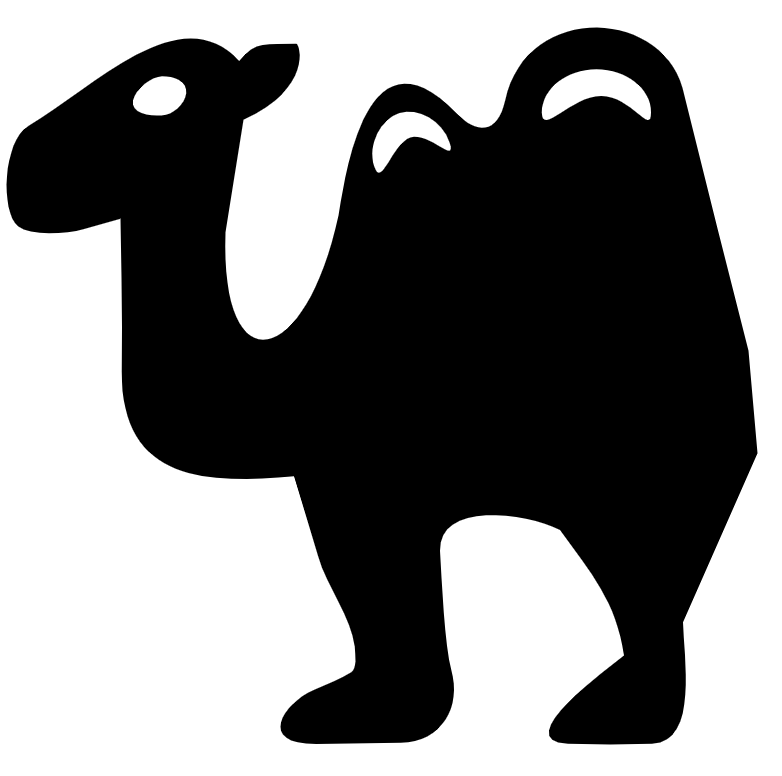
\includegraphics[width=0.15\linewidth]{figures/camelCase} \end{center}

Camel case has no symbols to separate words. Instead after the first
word every word starts with an upper case. Below are some examples of
names in Camel Case.

\begin{Shaded}
\begin{Highlighting}[]
\NormalTok{one}
\NormalTok{twoDf}
\NormalTok{two2Df}
\NormalTok{threeFourFive}
\NormalTok{threeFourFive2Vec}
\NormalTok{thisIsCamelCase}
\end{Highlighting}
\end{Shaded}

There are exceptions when you will want to break your naming style such
as when creating \textbf{vectors} to be used as columns for a
\textbf{data frame}.

\subsection{Wide vs Long coding}\label{wide-vs-long-coding}

If a command/\textbf{function} is only on one line then you were using
wide coding. This is good with short commands and \textbf{functions} but
is not very suitable for longer commands. Below are examples of long
commands over one line each.

\begin{Shaded}
\begin{Highlighting}[]
\CommentTok{#Create a data frame called df}
\NormalTok{df <-}\StringTok{ }\KeywordTok{data.frame}\NormalTok{(}\DataTypeTok{one =} \KeywordTok{c}\NormalTok{(}\DecValTok{2}\NormalTok{,}\DecValTok{4}\NormalTok{,}\DecValTok{6}\NormalTok{), }\DataTypeTok{three =} \KeywordTok{c}\NormalTok{(}\DecValTok{6}\NormalTok{,}\DecValTok{12}\NormalTok{,}\DecValTok{18}\NormalTok{), }\DataTypeTok{five =} \KeywordTok{c}\NormalTok{(}\DecValTok{10}\NormalTok{,}\DecValTok{20}\NormalTok{,}\DecValTok{30}\NormalTok{), }\DataTypeTok{row.names =} \KeywordTok{c}\NormalTok{(}\StringTok{"Two"}\NormalTok{, }\StringTok{"Four"}\NormalTok{, }\StringTok{"Six"}\NormalTok{))}
\CommentTok{#Create a data frame called beach_df_2}
\NormalTok{beach_df_}\DecValTok{2}\NormalTok{ <-}\StringTok{ }\KeywordTok{data.frame}\NormalTok{(}\DataTypeTok{Crab =} \KeywordTok{c}\NormalTok{(}\DecValTok{10}\NormalTok{,}\DecValTok{1}\NormalTok{,}\DecValTok{1}\NormalTok{,}\DecValTok{4}\NormalTok{) ,}\DataTypeTok{Oystercatcher =} \KeywordTok{c}\NormalTok{(}\DecValTok{5}\NormalTok{,}\DecValTok{6}\NormalTok{,}\DecValTok{4}\NormalTok{,}\DecValTok{4}\NormalTok{),}\DataTypeTok{Sandpiper =} \KeywordTok{c}\NormalTok{(}\DecValTok{1}\NormalTok{,}\DecValTok{1}\NormalTok{,}\DecValTok{2}\NormalTok{,}\DecValTok{3}\NormalTok{) ,}\DataTypeTok{Starfish =} \KeywordTok{c}\NormalTok{(}\DecValTok{3}\NormalTok{,}\DecValTok{3}\NormalTok{,}\DecValTok{7}\NormalTok{,}\DecValTok{4}\NormalTok{), }\DataTypeTok{row.names =} \KeywordTok{c}\NormalTok{(}\StringTok{"Formby"}\NormalTok{,}\StringTok{"West Kirby"}\NormalTok{,}\StringTok{"Crosby"}\NormalTok{,}\StringTok{"New Brighton"}\NormalTok{))}
\end{Highlighting}
\end{Shaded}

Compare the above with the below long coding where arguments are
separated by new lines.

\begin{Shaded}
\begin{Highlighting}[]
\CommentTok{#Create a data frame called df}
\NormalTok{df <-}\StringTok{ }\KeywordTok{data.frame}\NormalTok{(}\DataTypeTok{one =} \KeywordTok{c}\NormalTok{(}\DecValTok{2}\NormalTok{,}\DecValTok{4}\NormalTok{,}\DecValTok{6}\NormalTok{), }
                 \DataTypeTok{three =} \KeywordTok{c}\NormalTok{(}\DecValTok{6}\NormalTok{,}\DecValTok{12}\NormalTok{,}\DecValTok{18}\NormalTok{), }
                 \DataTypeTok{five =} \KeywordTok{c}\NormalTok{(}\DecValTok{10}\NormalTok{,}\DecValTok{20}\NormalTok{,}\DecValTok{30}\NormalTok{), }
                 \DataTypeTok{row.names =} \KeywordTok{c}\NormalTok{(}\StringTok{"Two"}\NormalTok{, }\StringTok{"Four"}\NormalTok{, }\StringTok{"Six"}\NormalTok{))}
\CommentTok{#Create a data frame called beach_df_2}
\NormalTok{beach_df_}\DecValTok{2}\NormalTok{ <-}\StringTok{ }\KeywordTok{data.frame}\NormalTok{(}\DataTypeTok{Crab =} \KeywordTok{c}\NormalTok{(}\DecValTok{10}\NormalTok{,}\DecValTok{1}\NormalTok{,}\DecValTok{1}\NormalTok{,}\DecValTok{4}\NormalTok{), }
                         \DataTypeTok{Oystercatcher =} \KeywordTok{c}\NormalTok{(}\DecValTok{5}\NormalTok{,}\DecValTok{6}\NormalTok{,}\DecValTok{4}\NormalTok{,}\DecValTok{4}\NormalTok{),}
                         \DataTypeTok{Sandpiper =} \KeywordTok{c}\NormalTok{(}\DecValTok{1}\NormalTok{,}\DecValTok{1}\NormalTok{,}\DecValTok{2}\NormalTok{,}\DecValTok{3}\NormalTok{),}
                         \DataTypeTok{Starfish =} \KeywordTok{c}\NormalTok{(}\DecValTok{3}\NormalTok{,}\DecValTok{3}\NormalTok{,}\DecValTok{7}\NormalTok{,}\DecValTok{4}\NormalTok{), }
                         \DataTypeTok{row.names =} \KeywordTok{c}\NormalTok{(}\StringTok{"Formby"}\NormalTok{,}\StringTok{"West Kirby"}\NormalTok{,}\StringTok{"Crosby"}\NormalTok{,}\StringTok{"New Brighton"}\NormalTok{))}
\end{Highlighting}
\end{Shaded}

Hopefully you will agree with me that the long coding is a lot easier
and quicker to read.

If you are interested in more about R style guide I would recommend
looking at the following resource: \url{https://style.tidyverse.org/}

\section{RStudio}\label{rstudio}

RStudio has many useful features which we have not covered. Let us
remedy this and cover a few.

\subsection{Global options}\label{global-options}

\begin{center}
\includegraphics[width=0.15\linewidth]{figures/global} \end{center}

To get to the RStudio Global Options click ``Tools'' in the RStudio
Toolbar, then from the drop down menu click ``Global Options..''. You
should see something similar to the below:

\begin{center}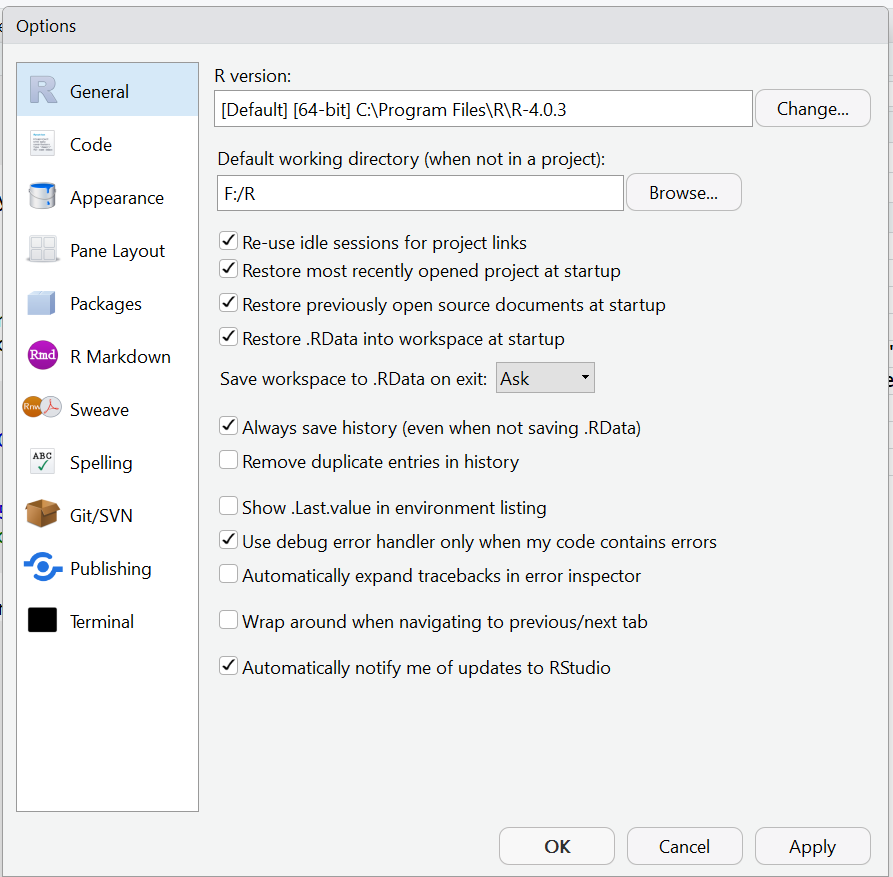
\includegraphics[width=0.4\linewidth]{figures/RStudio_global_options} \end{center}

Have a look through the ``General'', ``Code'', and ``Appearance''
sections. The other sections are more advanced and I would suggets you
ignore them currently.

Feel free to click on options in the ``Appearance'' section to see what
they do. If you do not like your choices you can click the ``Cancel''
button to negate your recent choices and close the window. If you want
to save your changes you can click the ``Apply'' button.

Also change the following for later.

\begin{enumerate}
\def\labelenumi{\arabic{enumi}.}
\tightlist
\item
  Go to Global options.
\item
  Click on the ``Code'' section on the left.
\item
  Click on the ``Completion'' tab at the top.
\item
  Ensure ``Show code completion:'' is set to ``Manually (Tab)''
\item
  Click ``Apply'' at the bottom followed by ``OK''.
\end{enumerate}

This will be useful for tab completion which we will cover shortly.

\begin{center}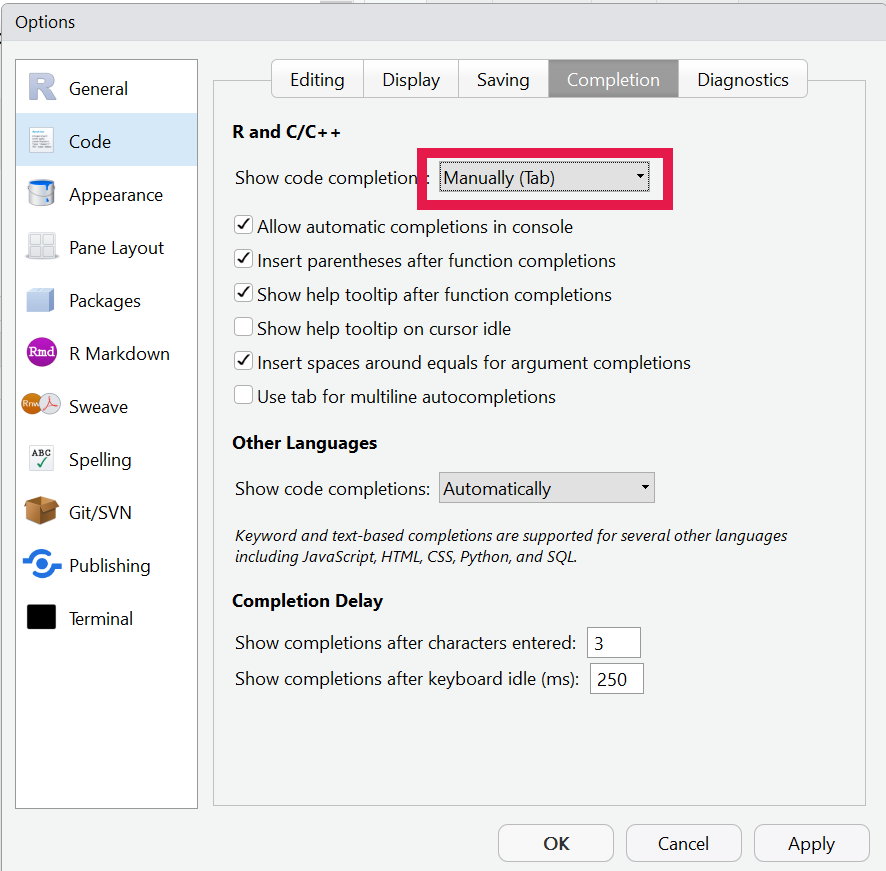
\includegraphics[width=0.4\linewidth]{figures/RStudio_manual_tab} \end{center}

\subsection{Sweep buttons}\label{sweep-buttons}

\begin{center}
\includegraphics[width=0.2\linewidth]{figures/sweep} \end{center}

Sweep buttons allow you to sweep away items you no longer want in
RStudio. There are two main sweep buttons, one for the \textbf{Console
window} and one for the \textbf{Environment pane}.

The sweep button for the \textbf{console window} will clear all the text
in the \textbf{console pane}. This is useful if you have filled the
\textbf{console} with lots of commands and \textbf{data frames}. This
sweep button will not actually affect any of your work so do not be
afraid to use it. The location of the sweep button is shown below.

\begin{center}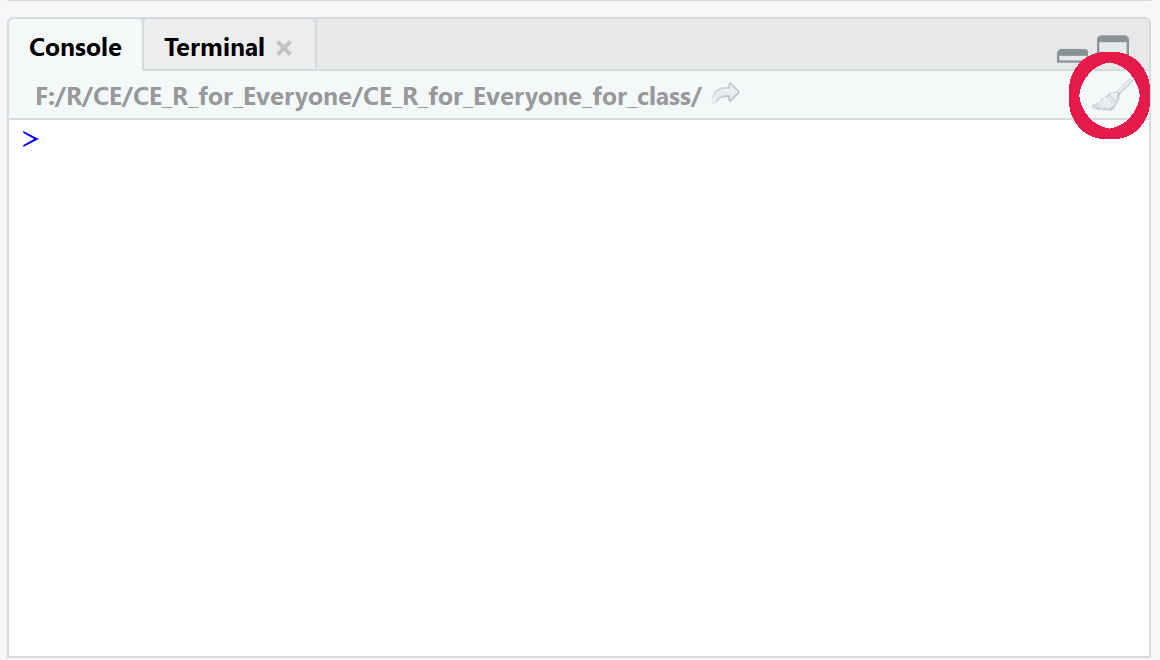
\includegraphics[width=0.4\linewidth]{figures/RStudio_console_sweep} \end{center}

The sweep button for the \textbf{Environment pane} is a bit more
dangerous. This sweep button will clear all the objects from your
environment. This will remove all the \textbf{variables} you have
created. This is not too bad if you have been using the \textbf{script
editor} to do your work as you can rerun all your commands to refill
your environment. The location of the sweep button is shown below.

\begin{center}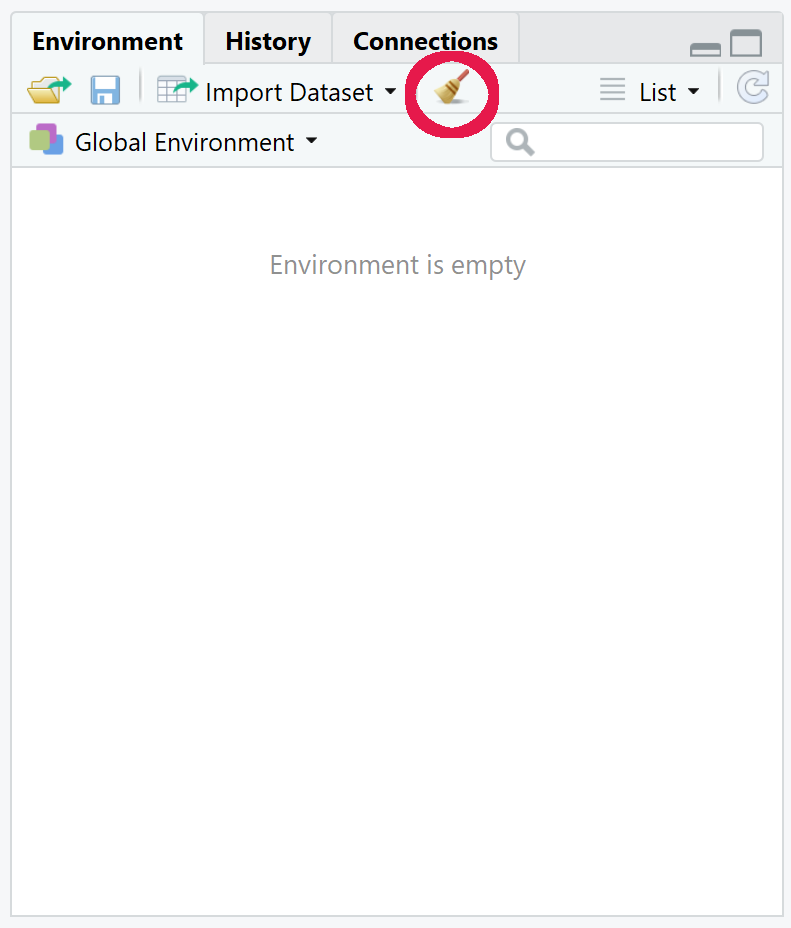
\includegraphics[width=0.4\linewidth]{figures/RStudio_env_sweep} \end{center}

\section{Multiplication table}\label{multiplication-table}

\begin{center}
\includegraphics[width=0.2\linewidth]{figures/multiplication} \end{center}

Hopefully you'll find the above useful. We will learn some new
\textbf{functions} but before that let us create a quick \textbf{data
frame}. You are going to make a multiplication table. The \textbf{data
frame} will be a 10 by 10 table with numbers one to ten as the row names
and the column names. The value in each cell/index will be equal to the
row name number times the column name number.

Before looking at the code below can you think of a way to do this?

The code below shows a method to create this \textbf{data frame}. I have
tried to show you a variety of methods to create the \textbf{vectors}
below for demonstration purposes. Look at each command and make sure you
understand how they work before continuing. In real life I would use one
of these methods rather than many differnet methods.

\textbf{Tip}: If you double click a word/name in the \textbf{script
editor} it will highlight it. You can then start to type to replace the
highlighted word.

\begin{Shaded}
\begin{Highlighting}[]
\CommentTok{#Vectors that will become columns}
\NormalTok{one <-}\StringTok{ }\DecValTok{1}\OperatorTok{:}\DecValTok{10}
\NormalTok{two <-}\StringTok{ }\NormalTok{one}\OperatorTok{*}\DecValTok{2}
\NormalTok{three <-}\StringTok{ }\NormalTok{one}\OperatorTok{+}\NormalTok{two}
\NormalTok{four <-}\StringTok{ }\KeywordTok{seq}\NormalTok{(}\DataTypeTok{from =} \DecValTok{4}\NormalTok{, }\DataTypeTok{to =} \DecValTok{40}\NormalTok{, }\DataTypeTok{by =} \DecValTok{4}\NormalTok{)}
\NormalTok{five <-}\StringTok{ }\NormalTok{(}\DecValTok{1}\OperatorTok{:}\DecValTok{10}\NormalTok{)}\OperatorTok{*}\DecValTok{5}
\NormalTok{six <-}\StringTok{ }\KeywordTok{seq}\NormalTok{(}\DataTypeTok{from =} \DecValTok{6}\NormalTok{, }\DataTypeTok{by =} \DecValTok{6}\NormalTok{, }\DataTypeTok{length.out =} \DecValTok{10}\NormalTok{)}
\NormalTok{seven <-}\StringTok{ }\NormalTok{one }\OperatorTok{*}\StringTok{ }\NormalTok{(}\KeywordTok{rep}\NormalTok{(}\DataTypeTok{x =} \DecValTok{7}\NormalTok{, }\DecValTok{10}\NormalTok{))}
\NormalTok{ate <-}\StringTok{ }\NormalTok{(}\DecValTok{1}\OperatorTok{:}\DecValTok{80}\NormalTok{)[((}\DecValTok{1}\OperatorTok{:}\DecValTok{80}\NormalTok{) }\OperatorTok\StringTok{ }\DecValTok{8}\NormalTok{) }\OperatorTok{==}\StringTok{ }\DecValTok{0}\NormalTok{]}
\NormalTok{nine <-}\StringTok{ }\NormalTok{one }\OperatorTok{*}\StringTok{ }\NormalTok{(}\KeywordTok{rep}\NormalTok{(}\DataTypeTok{x =} \DecValTok{9}\NormalTok{, }\DecValTok{10}\NormalTok{))}
\NormalTok{ten <-}\StringTok{ }\NormalTok{(}\KeywordTok{seq}\NormalTok{(}\DecValTok{100}\NormalTok{,}\DecValTok{1000}\NormalTok{,}\DecValTok{100}\NormalTok{))}\OperatorTok{/}\KeywordTok{rep}\NormalTok{(}\DecValTok{10}\NormalTok{,}\DecValTok{10}\NormalTok{)}
\CommentTok{#Vector for row name}
\NormalTok{row_names <-}\StringTok{ }\KeywordTok{c}\NormalTok{(}\StringTok{"one"}\NormalTok{,}\StringTok{"two"}\NormalTok{,}\StringTok{"three"}\NormalTok{,}\StringTok{"four"}\NormalTok{,}\StringTok{"five"}\NormalTok{,}
               \StringTok{"six"}\NormalTok{,}\StringTok{"sefen"}\NormalTok{,}\StringTok{"ate"}\NormalTok{,}\StringTok{"nine"}\NormalTok{,}\StringTok{"ten"}\NormalTok{)}
\CommentTok{#Create data frame}
\NormalTok{multiplication_df <-}\StringTok{ }\KeywordTok{data.frame}\NormalTok{(one, two, three,}
\NormalTok{                                four, five, six,}
\NormalTok{                                seven, ate, nine, ten,}
                                \DataTypeTok{row.names =}\NormalTok{ row_names)}
\end{Highlighting}
\end{Shaded}

Have a look at the resulting \textbf{data frame}. You may have noticed
that two of the row names and one of the column names is incorrect.
We'll use the \textbf{functions} \texttt{colnames()}and
\texttt{row.names()} along with indexes and assignment to change these.

\begin{Shaded}
\begin{Highlighting}[]
\CommentTok{#Change the 8th column name ("ate") to "eight"}
\KeywordTok{colnames}\NormalTok{(multiplication_df)[}\DecValTok{8}\NormalTok{] <-}\StringTok{ "eight"}
\CommentTok{#Change the 7th and 8th row names ("sefen" and "ate") to "seven" and "eight"}
\KeywordTok{row.names}\NormalTok{(multiplication_df)[}\DecValTok{7}\OperatorTok{:}\DecValTok{8}\NormalTok{] <-}\StringTok{ }\KeywordTok{c}\NormalTok{(}\StringTok{"seven"}\NormalTok{,}\StringTok{"eight"}\NormalTok{)}
\end{Highlighting}
\end{Shaded}

\section{Tab complete}\label{tab-complete}

\begin{center}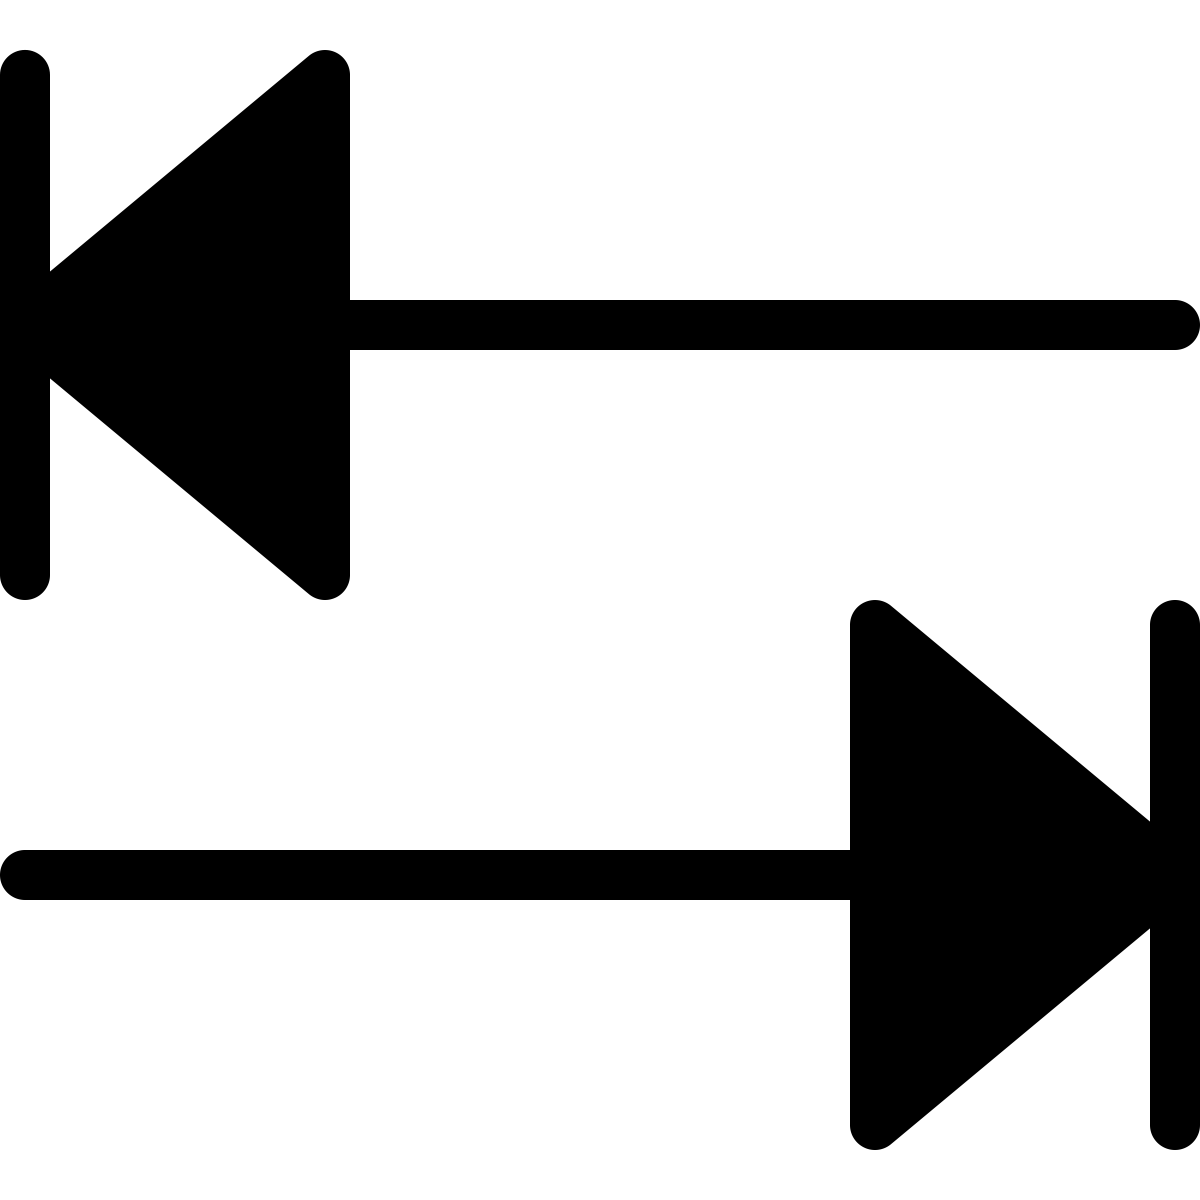
\includegraphics[width=0.15\linewidth]{figures/tab} \end{center}

Tab completion is a very useful method when coding in any language. It
takes some practice to get used to but it increases the speed of coding
and drastically reduces typos.

Before we continue, the tab key is the key above the ``CAPS'' key and
left of the `q' key. If you would like a demonstration of tab completion
please ask!

The first way to tab complete is to tab complete file names. First set
your working directory to the ``Tea'' directory in the
``Week\_4\_files'' directory you downloaded and unzipped for this week.
Then you will run the below command. However, when your cursor is in the
double quotes first press tab. This will hopefully show a dropdown of
selections. There are two ways to then get to your choice:

\begin{enumerate}
\def\labelenumi{\arabic{enumi}.}
\tightlist
\item
  Use the up and down arrow keys to move to the file name you want and
  then press enter to have the file name be autofilled.
\item
  Start typing your file name till it is the top choice of the drop down
  menu. You can then press enter to autofill the file name.
\end{enumerate}

In this case tab complete should only show ``tea\_consumption.csv'' as
it is the only file in your working directory.

\begin{Shaded}
\begin{Highlighting}[]
\NormalTok{tea_df <-}\StringTok{ }\KeywordTok{read.csv}\NormalTok{(}\StringTok{"tea_consumption.csv"}\NormalTok{, }\DataTypeTok{check.names=}\OtherTok{FALSE}\NormalTok{)}
\end{Highlighting}
\end{Shaded}

You may notice that we only provided the file name and the
\texttt{check.names=FALSE} for the \texttt{read.csv()}
\textbf{function}. This is because of the format of the input file. In
this case we do not want any of the input columns converted into row
names. Additionally, the file was comma separated and the default
separator to be used for \texttt{read.csv()} is commas. We will come
back to this \textbf{data frame} so either keep the \textbf{variable} in
your \textbf{environment} or keep the \textbf{read} code handy.

Let us \textbf{read} in another file using tab complete to autofill the
file name again. You will need to set your working directory to the
``Lanuguage'' directory in your ``Week\_4\_files'' directory first.

\begin{Shaded}
\begin{Highlighting}[]
\NormalTok{english_df <-}\StringTok{ }\KeywordTok{read.csv}\NormalTok{(}\StringTok{"english_speaking_population_of_countries.txt"}\NormalTok{, }
                   \DataTypeTok{sep =} \StringTok{"}\CharTok{\textbackslash{}t}\StringTok{"}\NormalTok{, }
                   \DataTypeTok{row.names =} \DecValTok{1}\NormalTok{,}
                   \DataTypeTok{check.names =} \OtherTok{FALSE}\NormalTok{)}
\end{Highlighting}
\end{Shaded}

Great!

The second way to use tab completion is to autofill \textbf{variable}
names, \textbf{function} names and options. To autofill a
\textbf{variable} or \textbf{function} name you can start typing the
name then press tab to get the dropdown menu.

Whilst in the \texttt{()} of a \textbf{function} you can press tab to
get a drop down menu of the option choices and press enter on the
highlighted choice to autofill it.

This only works if the name currently exists. I.e. you cannot autofill a
\textbf{variable name} if the \textbf{variable} is not in your
\textbf{environment}.

Continue using tab complete for the rest of the course. Practice makes
perfect.

If you really don't like it you don't have to use it.

Data from above files:

\begin{itemize}
\tightlist
\item
  \url{https://en.wikipedia.org/wiki/List_of_countries_by_tea_consumption_per_capita}
\item
  \url{https://en.wikipedia.org/wiki/List_of_countries_by_English-speaking_population}
\end{itemize}

\section{Tea}\label{tea}

\begin{center}
\includegraphics[width=0.2\linewidth]{figures/tea} \end{center}

We will have a quick look at the ``tea\_df''. This data shows the annual
consumption of tea per capita with a rank based on the highest to lowest
consumers.

Unfortunately the third column has the annual per capita consumption in
kilograms (KG) and pounds (LB) with the two values seperated by a
``\_``. Thankfully we can use the \textbf{function} \texttt{gsub()} to
fix this.

\texttt{gsub()} will look for a specified pattern and replace it with a
specified replacement. \texttt{gsub()} is only to be used for
\textbf{strings}.

Before fixing our \textbf{data frame} I'll show you some examples of
\texttt{gsub()}.

\begin{Shaded}
\begin{Highlighting}[]
\CommentTok{#Scalar string with mistake}
\NormalTok{sentence <-}\StringTok{ "The number 8 is spelt ate"}
\CommentTok{#gsub to print out line with mistake fixed}
\KeywordTok{gsub}\NormalTok{(}\DataTypeTok{pattern =} \StringTok{"ate"}\NormalTok{, }\DataTypeTok{replacement =} \StringTok{"eight"}\NormalTok{, sentence)}
\CommentTok{#We can assign the scalar with the fix}
\NormalTok{sentence <-}\StringTok{ }\KeywordTok{gsub}\NormalTok{(}\DataTypeTok{pattern =} \StringTok{"ate"}\NormalTok{, }\DataTypeTok{replacement =} \StringTok{"eight"}\NormalTok{, sentence)}

\CommentTok{#Vector with unwanted capital As}
\NormalTok{letter_vec <-}\StringTok{ }\KeywordTok{c}\NormalTok{(}\StringTok{"A"}\NormalTok{,}\StringTok{"Ab"}\NormalTok{,}\StringTok{"Abc"}\NormalTok{,}\StringTok{"Abcd"}\NormalTok{)}
\CommentTok{#Replace pattern A with replacement a}
\NormalTok{letter_vec <-}\StringTok{ }\KeywordTok{gsub}\NormalTok{(}\DataTypeTok{pattern =} \StringTok{"A"}\NormalTok{, }\DataTypeTok{replacement =} \StringTok{"a"}\NormalTok{, letter_vec)}

\CommentTok{#Vector with unwanted info after "_"}
\NormalTok{extra_info_vec <-}\StringTok{ }\KeywordTok{c}\NormalTok{(}\StringTok{"A_some"}\NormalTok{,}\StringTok{"B_nada"}\NormalTok{,}\StringTok{"C_stuff"}\NormalTok{,}\StringTok{"D_nill"}\NormalTok{)}
\CommentTok{#Replace the _ and everything after it with nothing}
\CommentTok{#We signify this with ".*" which means any character (.) repeated zero or more times (*)}
\KeywordTok{gsub}\NormalTok{(}\DataTypeTok{pattern =} \StringTok{"_.*"}\NormalTok{, }\DataTypeTok{replacement =} \StringTok{""}\NormalTok{, extra_info_vec)}

\CommentTok{#What if we use gsub() with numerics?}
\KeywordTok{gsub}\NormalTok{(}\DataTypeTok{pattern =} \DecValTok{5}\NormalTok{, }\DataTypeTok{replacement =} \DecValTok{2}\NormalTok{, }\DecValTok{1}\OperatorTok{:}\DecValTok{20}\NormalTok{)}
\CommentTok{#The output will be strings!}
\end{Highlighting}
\end{Shaded}

\texttt{.} and \texttt{*} are regular expressions. There are many
regular expressions but we will only use \texttt{.*} to represent ``all
strings''. The best part about this is we can put the \texttt{.*} after
a specific character to replace the specific character and everything
after it. Alternatively we can put the \texttt{.*} before a specific
character to replace the specific character and everything before it.

Let us carry this out with the ``tea\_df'' so it will hopefully make
more sense. We are going to do this so we can make a kilogram column and
a pound column.

\textbf{Note}: Make sure you have the ``tea\_df'' in your environment
before proceeding.

\begin{Shaded}
\begin{Highlighting}[]
\CommentTok{#Create a column for lb (pound). We'll copy the KG_LB_annual_per_capita column}
\NormalTok{tea_df}\OperatorTok{$}\NormalTok{lb <-}\StringTok{ }\NormalTok{tea_df}\OperatorTok{$}\NormalTok{KG_LB_annual_per_capita}
\CommentTok{#For the lb column we'll replace the "_" and everything before it with nothing}
\NormalTok{tea_df}\OperatorTok{$}\NormalTok{lb <-}\StringTok{ }\KeywordTok{gsub}\NormalTok{(}\DataTypeTok{pattern =} \StringTok{".*_"}\NormalTok{, }\DataTypeTok{replacement =} \StringTok{""}\NormalTok{, tea_df}\OperatorTok{$}\NormalTok{lb)}

\CommentTok{#Change the column name KG_LB_annual_per_capita to kg}
\KeywordTok{colnames}\NormalTok{(tea_df)[}\DecValTok{3}\NormalTok{] <-}\StringTok{ "kg"}
\CommentTok{#For the kg column we'll replace the "_" and everything after it with nothing}
\NormalTok{tea_df}\OperatorTok{$}\NormalTok{kg <-}\StringTok{ }\KeywordTok{gsub}\NormalTok{(}\DataTypeTok{pattern =} \StringTok{"_.*"}\NormalTok{, }\DataTypeTok{replacement =} \StringTok{""}\NormalTok{, tea_df}\OperatorTok{$}\NormalTok{kg)}

\CommentTok{#Since the columns initially contained "_" they are string columns}
\CommentTok{#Check if this is correct with the str() function}
\KeywordTok{str}\NormalTok{(tea_df)}
\CommentTok{#Change the kg and lb columns to numerics}
\NormalTok{tea_df}\OperatorTok{$}\NormalTok{kg <-}\StringTok{ }\KeywordTok{as.numeric}\NormalTok{(tea_df}\OperatorTok{$}\NormalTok{kg)}
\NormalTok{tea_df}\OperatorTok{$}\NormalTok{lb <-}\StringTok{ }\KeywordTok{as.numeric}\NormalTok{(tea_df}\OperatorTok{$}\NormalTok{lb)}
\CommentTok{#Check with str() to see if it is now numerics}
\KeywordTok{str}\NormalTok{(tea_df)}
\end{Highlighting}
\end{Shaded}

If you are interested in more regular expressions I would recommend
looking at the following resources:

\begin{itemize}
\tightlist
\item
  \url{https://r4ds.had.co.nz/strings.html\#matching-patterns-with-regular-expressions}
\item
  \url{https://rstudio.com/wp-content/uploads/2016/09/RegExCheatsheet.pdf}
\end{itemize}

\section{English speakers across the
world}\label{english-speakers-across-the-world}

\begin{center}
\includegraphics[width=0.2\linewidth]{figures/language} \end{center}

Now we will do some processing of the ``english\_df'' \textbf{data
frame}. This shows the various number of english speakers with info on
the number of those who have English as a first language and those who
have it as an additional language. View the \textbf{data frame} to see
its contents.

There are a lot of NA values. Looking at the values in the \textbf{data
frame} try to figure out the two reasons that these NA values are
present. Once you have had a thought you can have a look at the below
two reasons.

\begin{enumerate}
\def\labelenumi{\arabic{enumi}.}
\tightlist
\item
  Some countries have zero population of English first speakers and some
  countries have zero population of people who speak English as an
  additional language.
\item
  Some countries are missing data on the number of first and additional
  speakers, eg. Ukraine.
\end{enumerate}

We will fix these issues one by one. First let us change all NAs to the
number 0. The below method requires a lot of R knowledge to understand.
I admit I do not fully understand it and I googled to find the answer.
In this case the important part is that it works and it is a very short
command.

\begin{Shaded}
\begin{Highlighting}[]
\NormalTok{english_df[}\KeywordTok{is.na}\NormalTok{(english_df)] <-}\StringTok{ }\DecValTok{0}
\end{Highlighting}
\end{Shaded}

We have changed all NAs. However, some of the rows in the 3rd and 4th
column don't equal the 2nd column. We'll now remove these rows as they
have missing data and we don't want that here.

\begin{Shaded}
\begin{Highlighting}[]
\CommentTok{#1st method with multiple lines for clarity}
\CommentTok{#Create a vector of first language + additional language}
\NormalTok{english_total_vec <-}\StringTok{ }\NormalTok{english_df[,}\DecValTok{3}\NormalTok{] }\OperatorTok{+}\StringTok{ }\NormalTok{english_df[,}\StringTok{"As an additional language"}\NormalTok{]}
\CommentTok{#Compare the column of total english speakers against the vector we created above}
\CommentTok{#This will create a logical vector (TRUE or FALSE)}
\NormalTok{english_total_logical_vec <-}\StringTok{ }\NormalTok{english_df}\OperatorTok{$}\StringTok{`}\DataTypeTok{Total English speakers}\StringTok{`} \OperatorTok{==}\StringTok{ }\NormalTok{english_total_vec}
\CommentTok{#Now create a new data frame by indexxing the english_df rows by the logical vector}
\CommentTok{#This will mean all TRUE rows will be kept and all FALSE rows will not be kept}
\NormalTok{english_complete_datasets_df <-}\StringTok{ }\NormalTok{english_df[english_total_logical_vec,]}
\CommentTok{#Remove the vectors we do not need anymore}
\KeywordTok{rm}\NormalTok{(english_total_vec,english_total_logical_vec)}

\CommentTok{#2nd method is to carry out the above all in one command}
\NormalTok{english_complete_datasets_df_}\DecValTok{2}\NormalTok{ <-}\StringTok{ }
\StringTok{  }\NormalTok{english_df[}
\NormalTok{    (english_df}\OperatorTok{$}\StringTok{`}\DataTypeTok{As first language}\StringTok{`} \OperatorTok{+}\StringTok{ }\NormalTok{english_df}\OperatorTok{$}\StringTok{`}\DataTypeTok{As an additional language}\StringTok{`}\NormalTok{) }\OperatorTok{==}
\StringTok{      }\NormalTok{english_df}\OperatorTok{$}\StringTok{`}\DataTypeTok{Total English speakers}\StringTok{`}\NormalTok{,}
\NormalTok{    ]}

\CommentTok{#We can compare our two created data frames with the identical() function}
\KeywordTok{identical}\NormalTok{(english_complete_datasets_df,english_complete_datasets_df_}\DecValTok{2}\NormalTok{)}
\end{Highlighting}
\end{Shaded}

I would use the one command method but the multi line method is just as
valid. It doesn't matter if your R code is not as compact as possible.
The main things that matter are:

\begin{enumerate}
\def\labelenumi{\arabic{enumi}.}
\tightlist
\item
  Your code works. When writing your own code make sure you test it with
  small datasets first so you know it is doing what you think it is
  doing.
\item
  Your code is well annotated. This will help with the first step and it
  will help your future self and others who will read your code.
\item
  You can read and understand your own code (annotation helps). There is
  little point in code you cannot read. You will most likely need to
  debug code you write (I know I do). Write code in a way that you know
  you will be able to read. If this means doing little parts over
  multiple lines then do it that way.
\end{enumerate}

We will come back to the \textbf{data frames} ``tea\_df'' and
``english\_complete\_datasets\_df'' for the exercises. But let us go
onto 2 more topics.

\section{Identical}\label{identical}

\begin{center}\includegraphics[width=0.2\linewidth]{figures/identikeys} \end{center}

I touched on the \texttt{identical()} \textbf{function} above to compare
the two resulting \textbf{data frames}. \texttt{identical()} will
compare two objects and if the objects are exactly identical it will
print TRUE. If they are not exactly identical it will print FALSE. The
function can be given \textbf{scalars}, \textbf{vectors}, \textbf{data
frames} etc. Below are some examples

\begin{Shaded}
\begin{Highlighting}[]
\KeywordTok{identical}\NormalTok{(}\DecValTok{1}\NormalTok{,}\DecValTok{1}\NormalTok{)}
\KeywordTok{identical}\NormalTok{(}\DecValTok{1}\NormalTok{,}\DecValTok{2}\NormalTok{)}
\KeywordTok{identical}\NormalTok{(}\StringTok{"word"}\NormalTok{,}\StringTok{"word"}\NormalTok{)}
\KeywordTok{identical}\NormalTok{(}\StringTok{"word"}\NormalTok{,}\StringTok{"orb"}\NormalTok{)}
\KeywordTok{identical}\NormalTok{(}\DecValTok{1}\NormalTok{,}\StringTok{"1"}\NormalTok{)}
\KeywordTok{identical}\NormalTok{(}\StringTok{"one"}\NormalTok{,}\DecValTok{1}\NormalTok{)}
\KeywordTok{identical}\NormalTok{(}\DecValTok{1}\OperatorTok{:}\DecValTok{5}\NormalTok{,}\DecValTok{1}\OperatorTok{:}\DecValTok{5}\NormalTok{)}
\KeywordTok{identical}\NormalTok{(}\DecValTok{1}\OperatorTok{:}\DecValTok{5}\NormalTok{,}\DecValTok{6}\OperatorTok{:}\DecValTok{9}\NormalTok{)}
\KeywordTok{identical}\NormalTok{(}\DecValTok{1}\OperatorTok{:}\DecValTok{5}\NormalTok{,}\DecValTok{1}\OperatorTok{:}\DecValTok{6}\NormalTok{)}
\KeywordTok{identical}\NormalTok{(}\KeywordTok{c}\NormalTok{(}\StringTok{"a"}\NormalTok{,}\StringTok{"b"}\NormalTok{),}\KeywordTok{c}\NormalTok{(}\StringTok{"a"}\NormalTok{,}\StringTok{"b"}\NormalTok{))}
\KeywordTok{identical}\NormalTok{(}\KeywordTok{c}\NormalTok{(}\StringTok{"a"}\NormalTok{,}\StringTok{"b"}\NormalTok{),}\KeywordTok{c}\NormalTok{(}\StringTok{"c"}\NormalTok{,}\StringTok{"b"}\NormalTok{))}
\KeywordTok{identical}\NormalTok{(}\KeywordTok{c}\NormalTok{(}\StringTok{"a"}\NormalTok{,}\StringTok{"b"}\NormalTok{),}\KeywordTok{c}\NormalTok{(}\StringTok{"b"}\NormalTok{,}\StringTok{"a"}\NormalTok{))}
\KeywordTok{identical}\NormalTok{(english_df,english_df)}
\KeywordTok{identical}\NormalTok{(english_df,tea_df)}
\end{Highlighting}
\end{Shaded}

\section{Shortcuts}\label{shortcuts}

\begin{center}\includegraphics[width=0.3\linewidth]{figures/keyboard} \end{center}

RStudio has many keyboard shortcuts for the \textbf{Script editor}. Some
of these are common shortcuts used for other software and some are
unique to RStudio.

Below are a few:

\begin{itemize}
\tightlist
\item
  ``Ctrl + a'' : This will highlight all text in a \textbf{Script
  editor} that your cursor is in. This is useful to run all your code by
  highlighting it all and then pressing ``Ctrl + enter''. Be careful
  though as if you starting typing when all the text is highlighted it
  will delete it all.
\item
  ``Ctrl + z'' : This will undo your last typing action. You can undo
  your actions till the last time you saved your script. Very useful if
  you accidentally delete some text.
\item
  ``Ctrl + c'' : Copy highlighted text.
\item
  ``Ctrl + p'' : Paste text.
\item
  ``Ctrl + shift + c'' : This will put a \texttt{\#} at the start of
  each highlighted line. This is useful to annotate multiple lines at
  once. To unannotate the lines, highlight them again and use the
  shortcut.
\item
  ``Ctrl + f'' : This will bring the search and replace menu at the top
  of the \textbf{Script editor}.
\end{itemize}

There are a lot more shortcuts. If you want to see the full list go to
``Tools'' on the RStudio toolbar and then select ``Keyboard Shortcuts
Help''

Now time for exercises!

\chapter{Week 4 exercises}\label{week-4-exercises}

\begin{center}\includegraphics[width=0.2\linewidth]{figures/exercises} \end{center}

There has been a lot covered this week so these exercises will hopefully
be straightforward.

Please use your ``Exercises.R'' script for this, using annotations and
code sections to keep the contents clear and separated.

\section{Tea exercise}\label{tea-exercise}

\begin{center}\includegraphics[width=0.2\linewidth]{figures/tea} \end{center}

The first task you will carry out is printing out information from
``tea\_df''. Below is an example statement for the country Turkey:

``Turkey is the number 1 consumer of tea. It consumes 5.8kg of tea
annually per capita.''

Print out this satement for the countries Ireland, United Kingdom,
France, and Australia with their relevant information. Make sure the
kilogram value only has one decimal place.

\textbf{Tip}: You will require the \textbf{functions} \texttt{paste()}
and \texttt{round()} from week 2 and 1.

\section{English speakers across the world
exercise}\label{english-speakers-across-the-world-exercise}

\begin{center}\includegraphics[width=0.2\linewidth]{figures/language} \end{center}

The last exercise is to create the following table as a \textbf{data
frame} called ``english\_100mil\_df''. Use the
``english\_complete\_datasets\_df'' \textbf{data frame} as a start.

\begin{tabular}[t]{l|r|r|r|r|r}
\hline
  & Eligible population & Total English speakers & As first language & As an additional language & Fraction of population that are English speakers\\
\hline
United States & 296603003 & 283160411 & 234171556 & 48988855 & 0.9546782\\
\hline
Nigeria & 156493000 & 79000000 & 0 & 79000000 & 0.5048149\\
\hline
Philippines & 110000000 & 64025890 & 36935 & 63988955 & 0.5820535\\
\hline
Bangladesh & 163323100 & 30108031 & 709873 & 29398158 & 0.1843464\\
\hline
China & 1210000000 & 10000000 & 0 & 10000000 & 0.0082645\\
\hline
Brazil & 205000000 & 10542000 & 292000 & 10250000 & 0.0514244\\
\hline
Mexico & 120664000 & 15686262 & 0 & 15686262 & 0.1299995\\
\hline
Mean & 323154729 & 70360371 & 33601481 & 36758890 & 0.3450831\\
\hline
Total & 2262083103 & 492522594 & 235210364 & 257312230 & 0.2177297\\
\hline
\end{tabular}

The \textbf{data frame} only contains countries that have an eligible
population that is greater than 100 million (100000000). Ensure the
``Total'' row was not calculated using the ``Mean row''.

When you have created yours check it with the above one. Is your value
for the ``Total'' ``Fraction of population that are English speakers''
correct?.

Once you have created the \textbf{data frame} \textbf{write} it out as a
comma separated file with the function \texttt{write.table()} called
``English\_top\_7\_populated\_countries.csv''. Have the row and column
names surrounded by quotes in your file. Make sure there is an empty
value above your row names.

\section{Extra exercise}\label{extra-exercise}

\begin{center}\includegraphics[width=0.2\linewidth]{figures/multiplication} \end{center}

If you still have time this session and you do not have any questions
please attempt the following task:

Create a multiplication table like the one in the practice for this
week. However have the row and column names equal one to twelve.

Then \textbf{write} the \textbf{data frame} to a file. The name and
format of the file is up to you.

There is no solution to this in the next section.

\chapter{Week 4 exercise solutions}\label{week-4-exercise-solutions}

\begin{center}\includegraphics[width=0.2\linewidth]{figures/answers} \end{center}

\section{Tea solution}\label{tea-solution}

\begin{center}\includegraphics[width=0.2\linewidth]{figures/tea} \end{center}

First ensure you have the ``tea\_df'' loaded (remember your working
directory will need to be in the correct location first). Also it needs
to be preprocessed with the \texttt{gsub()} function.

\begin{Shaded}
\begin{Highlighting}[]
\NormalTok{tea_df <-}\StringTok{ }\KeywordTok{read.csv}\NormalTok{(}\StringTok{"tea_consumption.csv"}\NormalTok{, }\DataTypeTok{check.names=}\OtherTok{FALSE}\NormalTok{)}
\NormalTok{tea_df}\OperatorTok{$}\NormalTok{lb <-}\StringTok{ }\NormalTok{tea_df}\OperatorTok{$}\NormalTok{KG_LB_annual_per_capita}
\NormalTok{tea_df}\OperatorTok{$}\NormalTok{lb <-}\StringTok{ }\KeywordTok{gsub}\NormalTok{(}\DataTypeTok{pattern =} \StringTok{".*_"}\NormalTok{, }\DataTypeTok{replacement =} \StringTok{""}\NormalTok{, tea_df}\OperatorTok{$}\NormalTok{lb)}
\KeywordTok{colnames}\NormalTok{(tea_df)[}\DecValTok{3}\NormalTok{] <-}\StringTok{ "kg"}
\NormalTok{tea_df}\OperatorTok{$}\NormalTok{kg <-}\StringTok{ }\KeywordTok{gsub}\NormalTok{(}\DataTypeTok{pattern =} \StringTok{"_.*"}\NormalTok{, }\DataTypeTok{replacement =} \StringTok{""}\NormalTok{, tea_df}\OperatorTok{$}\NormalTok{kg)}
\NormalTok{tea_df}\OperatorTok{$}\NormalTok{kg <-}\StringTok{ }\KeywordTok{as.numeric}\NormalTok{(tea_df}\OperatorTok{$}\NormalTok{kg)}
\NormalTok{tea_df}\OperatorTok{$}\NormalTok{lb <-}\StringTok{ }\KeywordTok{as.numeric}\NormalTok{(tea_df}\OperatorTok{$}\NormalTok{lb)}
\end{Highlighting}
\end{Shaded}

Remember there are many ways to carry this out but here is one.

First create a \textbf{vector} with the names of the countries we want:

\begin{Shaded}
\begin{Highlighting}[]
\NormalTok{countries <-}\StringTok{ }\KeywordTok{c}\NormalTok{(}\StringTok{"Ireland"}\NormalTok{, }\StringTok{"United Kingdom"}\NormalTok{, }\StringTok{"France"}\NormalTok{, }\StringTok{"Australia"}\NormalTok{)}
\end{Highlighting}
\end{Shaded}

Set the row names to the countries for easy indexxing:

\textbf{Note}: Row name must be unique which is the case here.

\begin{Shaded}
\begin{Highlighting}[]
\KeywordTok{row.names}\NormalTok{(tea_df) <-}\StringTok{ }\NormalTok{tea_df}\OperatorTok{$}\NormalTok{Country}
\end{Highlighting}
\end{Shaded}

Create a \textbf{data frame} that only contains our countries of
interest. We use the \textbf{vector} as an index for the rows.

\begin{Shaded}
\begin{Highlighting}[]
\NormalTok{tea_df_subset <-}\StringTok{ }\NormalTok{tea_df[countries,]}
\end{Highlighting}
\end{Shaded}

Here because we are working with a temporary \textbf{variable} we will
overwrite the kg column so the values only contain one decimal place

\begin{Shaded}
\begin{Highlighting}[]
\NormalTok{tea_df_subset}\OperatorTok{$}\NormalTok{kg <-}\StringTok{ }\KeywordTok{round}\NormalTok{(}\DataTypeTok{x =}\NormalTok{ tea_df_subset}\OperatorTok{$}\NormalTok{kg, }\DataTypeTok{digits =} \DecValTok{1}\NormalTok{)}
\end{Highlighting}
\end{Shaded}

Last step is to print out the statement. We will use \texttt{paste0()}
which is exactly like \texttt{paste()} but the \texttt{sep\ =} option is
set to \texttt{""}.

\begin{Shaded}
\begin{Highlighting}[]
\KeywordTok{paste0}\NormalTok{(tea_df_subset}\OperatorTok{$}\NormalTok{Country, }\StringTok{" is the number "}\NormalTok{, tea_df_subset}\OperatorTok{$}\NormalTok{Rank,}
       \StringTok{" consumer of tea. It consumes "}\NormalTok{, tea_df_subset}\OperatorTok{$}\NormalTok{kg, }\StringTok{"kg of tea annually per capita."}\NormalTok{)}
\end{Highlighting}
\end{Shaded}

\section{English speakers across the world
solution}\label{english-speakers-across-the-world-solution}

\begin{center}\includegraphics[width=0.2\linewidth]{figures/language} \end{center}

First make sure the \textbf{data frame} is created. Remember to set your
working directory to where the file is.

\begin{Shaded}
\begin{Highlighting}[]
\NormalTok{english_df <-}\StringTok{ }\KeywordTok{read.csv}\NormalTok{(}\StringTok{"english_speaking_population_of_countries.txt"}\NormalTok{, }
                   \DataTypeTok{sep =} \StringTok{"}\CharTok{\textbackslash{}t}\StringTok{"}\NormalTok{, }
                   \DataTypeTok{row.names =} \DecValTok{1}\NormalTok{,}
                   \DataTypeTok{check.names =} \OtherTok{FALSE}\NormalTok{)}
\NormalTok{english_df[}\KeywordTok{is.na}\NormalTok{(english_df)] <-}\StringTok{ }\DecValTok{0}
\NormalTok{english_complete_datasets_df <-}\StringTok{ }
\StringTok{  }\NormalTok{english_df[}
\NormalTok{    (english_df}\OperatorTok{$}\StringTok{`}\DataTypeTok{As first language}\StringTok{`} \OperatorTok{+}\StringTok{ }\NormalTok{english_df}\OperatorTok{$}\StringTok{`}\DataTypeTok{As an additional language}\StringTok{`}\NormalTok{) }\OperatorTok{==}
\StringTok{      }\NormalTok{english_df}\OperatorTok{$}\StringTok{`}\DataTypeTok{Total English speakers}\StringTok{`}\NormalTok{,}
\NormalTok{    ]}
\end{Highlighting}
\end{Shaded}

Create new \textbf{data frame} only containing countries with an
eligible population of \textgreater{} 100 million.

\begin{Shaded}
\begin{Highlighting}[]
\NormalTok{english_100mil_df <-}\StringTok{ }\NormalTok{english_complete_datasets_df[}
\NormalTok{  english_complete_datasets_df}\OperatorTok{$}\StringTok{`}\DataTypeTok{Eligible population}\StringTok{`} \OperatorTok{>}\StringTok{ }\DecValTok{100000000}\NormalTok{,}
\NormalTok{  ]}
\end{Highlighting}
\end{Shaded}

Create column with fraction of total english speakers against population

\begin{Shaded}
\begin{Highlighting}[]
\NormalTok{english_100mil_df}\OperatorTok{$}\StringTok{`}\DataTypeTok{Fraction of population that are English speakers}\StringTok{`}\NormalTok{ <-}\StringTok{ }
\StringTok{  }\NormalTok{english_100mil_df}\OperatorTok{$}\StringTok{`}\DataTypeTok{Total English speakers}\StringTok{`} \OperatorTok{/}
\StringTok{  }\NormalTok{english_100mil_df}\OperatorTok{$}\StringTok{`}\DataTypeTok{Eligible population}\StringTok{`}
\end{Highlighting}
\end{Shaded}

Create row with mean values

\begin{Shaded}
\begin{Highlighting}[]
\NormalTok{english_100mil_df[}\StringTok{"Mean"}\NormalTok{,] <-}\StringTok{ }\KeywordTok{colMeans}\NormalTok{(english_100mil_df)}
\end{Highlighting}
\end{Shaded}

Create row with totals

\begin{Shaded}
\begin{Highlighting}[]
\NormalTok{english_100mil_df[}\StringTok{"Total"}\NormalTok{,}\DecValTok{1}\OperatorTok{:}\DecValTok{4}\NormalTok{] <-}\StringTok{ }\KeywordTok{colSums}\NormalTok{(english_100mil_df[}\DecValTok{1}\OperatorTok{:}\DecValTok{7}\NormalTok{,}\DecValTok{1}\OperatorTok{:}\DecValTok{4}\NormalTok{])}
\end{Highlighting}
\end{Shaded}

Create the total fraction of english speakers

\begin{Shaded}
\begin{Highlighting}[]
\NormalTok{english_100mil_df[}\StringTok{"Total"}\NormalTok{,}\StringTok{"Fraction of population that are English speakers"}\NormalTok{] <-}\StringTok{ }
\StringTok{  }\NormalTok{english_100mil_df[}\StringTok{"Total"}\NormalTok{,}\StringTok{"Total English speakers"}\NormalTok{] }\OperatorTok{/}
\StringTok{  }\NormalTok{english_100mil_df[}\StringTok{"Total"}\NormalTok{,}\StringTok{"Eligible population"}\NormalTok{]}
\end{Highlighting}
\end{Shaded}

\textbf{Write} the data as a file

\begin{Shaded}
\begin{Highlighting}[]
\KeywordTok{write.table}\NormalTok{(}\DataTypeTok{x =}\NormalTok{ english_100mil_df, }
            \DataTypeTok{file =} \StringTok{"English_top_7_populated_countries.csv"}\NormalTok{, }
            \DataTypeTok{col.names=}\OtherTok{NA}\NormalTok{,}
            \DataTypeTok{quote =} \OtherTok{TRUE}\NormalTok{, }
            \DataTypeTok{sep =} \StringTok{","}\NormalTok{)}
\end{Highlighting}
\end{Shaded}

\chapter{Week 5 - Plots: Histograms and Line
graphs}\label{week-5---plots-histograms-and-line-graphs}

\begin{center}\includegraphics[width=0.2\linewidth]{figures/palette} \end{center}

This week we will learn how to create two different types of plots;
Histograms and Line graphs. I have chosen these two types of plots first
as they are relatively straightforward to create.

\section{Histogram}\label{histogram}

\begin{center}\includegraphics[width=0.2\linewidth]{figures/histogram} \end{center}

A histogram consists of bars showing the frequency of variables present
in numbered ranges (bins). This allows you to see an approximate
distribution of numerical data.

We are starting with histograms as the \textbf{function}
\texttt{hist()}, which creates a histogram, only requires one
\textbf{vector}.

The following code creates a numerical \textbf{vector} and then produces
a histogram. When you run the \texttt{hist()} command a plot should
appear in your \textbf{``Plots'' pane} of the \textbf{MISC window}.

\begin{Shaded}
\begin{Highlighting}[]
\NormalTok{numeric_vec <-}\StringTok{ }\DecValTok{1}\OperatorTok{:}\DecValTok{40}
\KeywordTok{hist}\NormalTok{(numeric_vec)}
\end{Highlighting}
\end{Shaded}

You will notice that the histogram is not very interesting. There are 8
bars all of equal size. This is because we plotted the numbers from 1-40
so numbers 1-5 are counted in the first bar/bin, 6-10 in the second
bar/bin and so forth. To get a more interesting histogram we will create
a more interesting \textbf{vector}.

Histograms are good to see the numerical distribution of data. In this
case we are going to look at the number of cities (with greater than
300,000 population) in EU countries
(\url{https://en.Wikipedia.org/wiki/List_of_cities_in_the_European_Union_by_population_within_city_limits}).

The first step is to create a \textbf{vector} with the numbers of cities
in EU countries, however we won't know what countries these correspond
to yet. Then we will create a histogram and set the colour of the bars
with the option \texttt{col\ =}.

\begin{Shaded}
\begin{Highlighting}[]
\NormalTok{eu_cities <-}\StringTok{ }\KeywordTok{c}\NormalTok{(}\DecValTok{1}\NormalTok{, }\DecValTok{1}\NormalTok{, }\DecValTok{3}\NormalTok{, }\DecValTok{1}\NormalTok{, }\DecValTok{2}\NormalTok{,}
               \DecValTok{2}\NormalTok{, }\DecValTok{1}\NormalTok{, }\DecValTok{1}\NormalTok{, }\DecValTok{6}\NormalTok{, }\DecValTok{22}\NormalTok{,}
               \DecValTok{2}\NormalTok{, }\DecValTok{1}\NormalTok{, }\DecValTok{1}\NormalTok{, }\DecValTok{10}\NormalTok{, }\DecValTok{1}\NormalTok{,}
               \DecValTok{1}\NormalTok{, }\DecValTok{4}\NormalTok{, }\DecValTok{9}\NormalTok{, }\DecValTok{1}\NormalTok{, }\DecValTok{7}\NormalTok{,}
               \DecValTok{1}\NormalTok{, }\DecValTok{12}\NormalTok{, }\DecValTok{3}\NormalTok{)}
\KeywordTok{hist}\NormalTok{(eu_cities, }\DataTypeTok{col =} \StringTok{"orange"}\NormalTok{)}
\end{Highlighting}
\end{Shaded}

With that histogram we can see that most EU countries have 1-5 cities
with a few having a much larger amount. As most of the time you will not
be working with just \textbf{vectors} let us make a \textbf{data frame}
containing the number of EU cities and the population of the EU
countries.

The population numbers will be in millions to the closest 1 decimal
place and consist of the 2020 Eurostat figures from:
\url{https://en.Wikipedia.org/wiki/List_of_European_Union_member_states_by_population}

\begin{Shaded}
\begin{Highlighting}[]
\NormalTok{eu_country_names <-}\StringTok{ }\KeywordTok{c}\NormalTok{(}\StringTok{"Austria"}\NormalTok{, }\StringTok{"Belgium"}\NormalTok{, }\StringTok{"Bulgaria"}\NormalTok{, }\StringTok{"Croatia"}\NormalTok{, }\StringTok{"Czech Republic"}\NormalTok{, }
                      \StringTok{"Denmark"}\NormalTok{, }\StringTok{"Estonia"}\NormalTok{, }\StringTok{"Finland"}\NormalTok{, }\StringTok{"France"}\NormalTok{, }\StringTok{"Germany"}\NormalTok{, }
                      \StringTok{"Greece"}\NormalTok{, }\StringTok{"Hungary"}\NormalTok{, }\StringTok{"Ireland"}\NormalTok{, }\StringTok{"Italy"}\NormalTok{, }\StringTok{"Latvia"}\NormalTok{, }
                      \StringTok{"Lithuania"}\NormalTok{, }\StringTok{"Netherlands"}\NormalTok{, }\StringTok{"Poland"}\NormalTok{, }\StringTok{"Portugal"}\NormalTok{, }\StringTok{"Romania"}\NormalTok{, }
                      \StringTok{"Slovakia"}\NormalTok{, }\StringTok{"Spain"}\NormalTok{, }\StringTok{"Sweden"}\NormalTok{)}
\NormalTok{eu_pop <-}\StringTok{ }\KeywordTok{c}\NormalTok{(}\FloatTok{8.9}\NormalTok{, }\FloatTok{11.5}\NormalTok{, }\FloatTok{7.0}\NormalTok{, }\FloatTok{4.1}\NormalTok{, }\FloatTok{10.7}\NormalTok{,}
            \FloatTok{5.8}\NormalTok{, }\FloatTok{1.3}\NormalTok{, }\FloatTok{5.5}\NormalTok{, }\FloatTok{67.1}\NormalTok{, }\FloatTok{83.2}\NormalTok{,}
            \FloatTok{10.7}\NormalTok{, }\FloatTok{9.8}\NormalTok{, }\FloatTok{5.0}\NormalTok{, }\FloatTok{60.2}\NormalTok{, }\FloatTok{1.9}\NormalTok{,}
            \FloatTok{2.8}\NormalTok{, }\FloatTok{17.4}\NormalTok{, }\FloatTok{38.0}\NormalTok{, }\FloatTok{10.3}\NormalTok{, }\FloatTok{19.3}\NormalTok{,}
            \FloatTok{5.5}\NormalTok{, }\FloatTok{47.3}\NormalTok{, }\FloatTok{10.3}\NormalTok{)}
\NormalTok{eu_df <-}\StringTok{ }\KeywordTok{data.frame}\NormalTok{(eu_cities,eu_pop,}
                    \DataTypeTok{row.names =}\NormalTok{ eu_country_names)}
\end{Highlighting}
\end{Shaded}

We will quickly create a histogram for the population numbers. We'll
make the bar colours purple and we'll make the x axis label ``2020
Eurostat population number in millions'' with the \texttt{xlab\ =}
option.

\begin{Shaded}
\begin{Highlighting}[]
\KeywordTok{hist}\NormalTok{(eu_df}\OperatorTok{$}\NormalTok{eu_pop, }\DataTypeTok{col =} \StringTok{"purple"}\NormalTok{,}
     \DataTypeTok{xlab =} \StringTok{"2020 Eurostat population number in millions"}\NormalTok{)}
\end{Highlighting}
\end{Shaded}

We have a similar pattern as with the number of cities (most have low
numbers, some high numbers).

We can quickly check if the countries with the high number of cities
also have the high populations by creating a new column equal to
population / number of cities. This will give is nice ratios. We can
plot the distribution of these ratios in a histogram.

For this histogram we will also add a title to the plot with the option
\texttt{main\ =}. Additionally we will choose a different colour. Having
different colours and main titles makes it easier for you to instantly
know which plot you are looking at.

\begin{Shaded}
\begin{Highlighting}[]
\CommentTok{#Create ratio column}
\NormalTok{eu_df}\OperatorTok{$}\NormalTok{pop_cities_ratio <-}\StringTok{ }\NormalTok{eu_df}\OperatorTok{$}\NormalTok{eu_pop }\OperatorTok{/}\StringTok{ }\NormalTok{eu_df}\OperatorTok{$}\NormalTok{eu_cities}
\CommentTok{#Histogram of ratio distribution}
\KeywordTok{hist}\NormalTok{(eu_df}\OperatorTok{$}\NormalTok{pop_cities_ratio, }\DataTypeTok{col =} \StringTok{"blue"}\NormalTok{,}
     \DataTypeTok{xlab =} \StringTok{"Ratio of population (millions) to numer of cities"}\NormalTok{,}
     \DataTypeTok{main =} \StringTok{"EU countries ratio of population to cities"}\NormalTok{)}
\end{Highlighting}
\end{Shaded}

Looking at the plot most countries seem to have a ratio of 2-6 million
citizens to every city. However, it is still not a perfect match with
some lower and some higher ratios. Of course a result is a result and we
have hopefully found out something new.

Before we go onto line graphs I'll show you how to look at your previous
plots. In the \textbf{Plots pane} of the \textbf{MISC window} there are
two arrows on the top left. You can use these to go backwards and
forwards between the plots you have created since you opened RStudio.
Give it a go!

\begin{center}\includegraphics[width=0.4\linewidth]{figures/RStudio_plot_pane_arrows} \end{center}

\section{Line graphs}\label{line-graphs}

\begin{center}\includegraphics[width=0.2\linewidth]{figures/line_graph} \end{center}

Line graphs are perfect for showing change over time. Knowing this we'll
go back to a data set we have touched before, the file
``UK\_retail.txt'' from week 3. This file showed the success of four
different retail sectors in the UK from September 2017 to September
2020.

\subsection{Read in data}\label{read-in-data}

First step is to set your working directory to the ``Week\_3\_files''
directory so you can then read in the data. Once the \textbf{data frame}
is created we will remove all non 2020 information.

\begin{Shaded}
\begin{Highlighting}[]
\NormalTok{retail_df <-}\StringTok{ }\KeywordTok{read.csv}\NormalTok{(}\StringTok{"UK_retail.txt"}\NormalTok{, }\DataTypeTok{sep =} \StringTok{"}\CharTok{\textbackslash{}t}\StringTok{"}\NormalTok{, }\DataTypeTok{row.names =} \DecValTok{1}\NormalTok{, }\DataTypeTok{check.names =} \OtherTok{FALSE}\NormalTok{)}
\NormalTok{retail_df <-}\StringTok{ }\NormalTok{retail_df[}\DecValTok{29}\OperatorTok{:}\DecValTok{37}\NormalTok{,]}
\end{Highlighting}
\end{Shaded}

Before we continue have a look at the \textbf{data frame} and make sure
you are comfortable with what it contains.

\subsection{Plotting a line graph}\label{plotting-a-line-graph}

We are going to plot the entire information for the Food sector. We will
use the \textbf{function} \texttt{plot()} with the option
\texttt{type\ =\ "l"}. This will produce a plot of type ``line''
(\texttt{"l"}).

This requires we provide a numeric \textbf{vector} for the x axis
(option \texttt{x\ =}) and the y axis (option \texttt{y\ =}). Currently
our month and year information is in the row names as strings.

Therefore before we plot the information we will create a new column
called ``time\_point'' with the numbers 1 to the number of rows. We will
carry this out with the \textbf{function} \texttt{nrow()} which produces
one number equal to the number of rows in the specified \textbf{data
frame}.

We won't use it here but the \textbf{function} \texttt{ncol()} is
similar to \texttt{nrow()} but for the number of columns.

\begin{Shaded}
\begin{Highlighting}[]
\CommentTok{#Produce time_point column}
\NormalTok{retail_df}\OperatorTok{$}\NormalTok{time_point <-}\StringTok{ }\DecValTok{1}\OperatorTok{:}\NormalTok{(}\KeywordTok{nrow}\NormalTok{(retail_df))}
\CommentTok{#Produce line plot of the food sector over time point.}
\KeywordTok{plot}\NormalTok{(}\DataTypeTok{y =}\NormalTok{ retail_df}\OperatorTok{$}\NormalTok{Food, retail_df}\OperatorTok{$}\NormalTok{time_point, }\DataTypeTok{type =} \StringTok{"l"}\NormalTok{)}
\end{Highlighting}
\end{Shaded}

\subsection{Adding lines to a plot}\label{adding-lines-to-a-plot}

This is looking decent but you normally want more than one line in a
line graph. Thankfully we can do this with the \textbf{function}
\texttt{lines()}. We can add the other three sectors to the line graph
like below:

\textbf{Tip}: Remember to use tab completion to auto fill
\textbf{function}, \textbf{variable}, and column names as well as for
\textbf{function} options.

\begin{Shaded}
\begin{Highlighting}[]
\KeywordTok{lines}\NormalTok{(}\DataTypeTok{y =}\NormalTok{ retail_df}\OperatorTok{$}\StringTok{`}\DataTypeTok{Non-food}\StringTok{`}\NormalTok{, }\DataTypeTok{x =}\NormalTok{ retail_df}\OperatorTok{$}\NormalTok{time_point)}
\KeywordTok{lines}\NormalTok{(}\DataTypeTok{y =}\NormalTok{ retail_df}\OperatorTok{$}\StringTok{`}\DataTypeTok{Non-store}\StringTok{`}\NormalTok{, }\DataTypeTok{x =}\NormalTok{ retail_df}\OperatorTok{$}\NormalTok{time_point)}
\KeywordTok{lines}\NormalTok{(}\DataTypeTok{y =}\NormalTok{ retail_df}\OperatorTok{$}\NormalTok{Fuel, }\DataTypeTok{x =}\NormalTok{ retail_df}\OperatorTok{$}\NormalTok{time_point)}
\end{Highlighting}
\end{Shaded}

We have created the line graph with all the sectors. However all the
data is not visible.

\subsection{Axis limits}\label{axis-limits}

To fix this we need to make sure all the data is within the graph. When
the \texttt{plot()} \textbf{function} was run it created the y limits
based on the Food sector which has a minimum and maximum value of 101.5
and 111.3. Unfortunately the other sectors barely fit in this range.

To prevent this issue we can use the \texttt{plot()} option of
\texttt{ylim\ =}. This option is provided with a \textbf{vector} of 2
numbers. The first number is where the y axis will start. The second
number is where the y axis will end.

To find out where the y axis will end we will use the \texttt{max()}
\textbf{function}. This will give one number which is equal to the
highest number found in a numeric \textbf{object}. This \textbf{object}
can be a \textbf{scalar}, \textbf{vector}, or a \textbf{data frame}.

We will use the \textbf{function} \texttt{min()} just like
\texttt{max()} to find where the y axis should start.

Let us therefore recreate the plot with an appropriate y axis range.

\textbf{Note}: Some times it is more appropriate to set values for the y
limits (i.e.~starting the y axis at 0). In this case 100 is the baseline
value so it would be inappropriate to start at 0.

\textbf{Tip}: Copying your past code in the script editor and editing it
will make the following examples a lot quicker to carry out.

\begin{Shaded}
\begin{Highlighting}[]
\CommentTok{#Minimum and maximum for y axis}
\CommentTok{#Provide the function a subset of the retail_df}
\CommentTok{#so it is not using the time_point column}
\NormalTok{min_y <-}\StringTok{ }\KeywordTok{min}\NormalTok{(retail_df[,}\DecValTok{1}\OperatorTok{:}\DecValTok{4}\NormalTok{])}
\NormalTok{max_y <-}\StringTok{ }\KeywordTok{max}\NormalTok{(retail_df[,}\OperatorTok{-}\DecValTok{5}\NormalTok{])}
\CommentTok{#Produce line plot of the food sector over time point.}
\CommentTok{#Set y limits (min,max)}
\KeywordTok{plot}\NormalTok{(}\DataTypeTok{y =}\NormalTok{ retail_df}\OperatorTok{$}\NormalTok{Food, retail_df}\OperatorTok{$}\NormalTok{time_point, }\DataTypeTok{type =} \StringTok{"l"}\NormalTok{,}
     \DataTypeTok{ylim =} \KeywordTok{c}\NormalTok{(min_y,max_y))}
\CommentTok{#Add lines}
\KeywordTok{lines}\NormalTok{(}\DataTypeTok{y =}\NormalTok{ retail_df}\OperatorTok{$}\StringTok{`}\DataTypeTok{Non-food}\StringTok{`}\NormalTok{, }\DataTypeTok{x =}\NormalTok{ retail_df}\OperatorTok{$}\NormalTok{time_point)}
\KeywordTok{lines}\NormalTok{(}\DataTypeTok{y =}\NormalTok{ retail_df}\OperatorTok{$}\StringTok{`}\DataTypeTok{Non-store}\StringTok{`}\NormalTok{, }\DataTypeTok{x =}\NormalTok{ retail_df}\OperatorTok{$}\NormalTok{time_point)}
\KeywordTok{lines}\NormalTok{(}\DataTypeTok{y =}\NormalTok{ retail_df}\OperatorTok{$}\NormalTok{Fuel, }\DataTypeTok{x =}\NormalTok{ retail_df}\OperatorTok{$}\NormalTok{time_point)}
\end{Highlighting}
\end{Shaded}

Great! That is much better. We can now see that two lines fall after
time\_point 2 whilst one increases.

\subsection{Axis labels}\label{axis-labels}

Numbers on the x axis are not ideal in this case. We will therefore use
the \texttt{axis()} function to set our own x axis labels. We will use
the following options for this:

\begin{itemize}
\tightlist
\item
  \texttt{1}: The first option to \texttt{axis()} indicates the location
  of the axis labels. \texttt{1} indicates they will be located on the x
  axis (below).
\item
  \texttt{at\ =\ retail\_df\$time\_point}: This indicates where the
  points tic marks will be drawn.
\item
  \texttt{labels\ =\ row.names(retail\_df)}: A character \textbf{vector}
  for the labels to be placed at the tick marks.
\end{itemize}

For more info for \texttt{axis()} run the command \texttt{?axis} to see
its help page.

To use the \texttt{axis()} \textbf{function} correctly we need to make
sure there are no preexisting labels and tick marks on the x axis or
else the new labels will go on top of the old. To do this we provide the
\texttt{plot()} \textbf{function} with the option
\texttt{naxt\ =\textquotesingle{}n\textquotesingle{}}, i.e.~no x axis
ticks.

\begin{Shaded}
\begin{Highlighting}[]
\CommentTok{#Produce line plot of the food sector over time point.}
\CommentTok{#Ensure x axis ticks and labels are not displayed}
\KeywordTok{plot}\NormalTok{(}\DataTypeTok{y =}\NormalTok{ retail_df}\OperatorTok{$}\NormalTok{Food, retail_df}\OperatorTok{$}\NormalTok{time_point, }\DataTypeTok{type =} \StringTok{"l"}\NormalTok{,}
     \DataTypeTok{ylim =} \KeywordTok{c}\NormalTok{(min_y,max_y), }\DataTypeTok{xaxt =} \StringTok{'n'}\NormalTok{)}
\CommentTok{#Add row names (month and date strings) as x axix labels}
\KeywordTok{axis}\NormalTok{(}\DecValTok{1}\NormalTok{, }\DataTypeTok{at =}\NormalTok{ retail_df}\OperatorTok{$}\NormalTok{time_point, }\DataTypeTok{labels =} \KeywordTok{row.names}\NormalTok{(retail_df))}
\CommentTok{#Add lines}
\KeywordTok{lines}\NormalTok{(}\DataTypeTok{y =}\NormalTok{ retail_df}\OperatorTok{$}\StringTok{`}\DataTypeTok{Non-food}\StringTok{`}\NormalTok{, }\DataTypeTok{x =}\NormalTok{ retail_df}\OperatorTok{$}\NormalTok{time_point)}
\KeywordTok{lines}\NormalTok{(}\DataTypeTok{y =}\NormalTok{ retail_df}\OperatorTok{$}\StringTok{`}\DataTypeTok{Non-store}\StringTok{`}\NormalTok{, }\DataTypeTok{x =}\NormalTok{ retail_df}\OperatorTok{$}\NormalTok{time_point)}
\KeywordTok{lines}\NormalTok{(}\DataTypeTok{y =}\NormalTok{ retail_df}\OperatorTok{$}\NormalTok{Fuel, }\DataTypeTok{x =}\NormalTok{ retail_df}\OperatorTok{$}\NormalTok{time_point)}
\end{Highlighting}
\end{Shaded}

When the plot is generated there may be only some labels showing for the
x axis. If you would like to show them all increase the size of the
\textbf{MISC window}.

\subsection{Plot titles}\label{plot-titles}

Before we colour the lines different colours, let us add a main title
and provided better x and y axis with better titles.

\begin{Shaded}
\begin{Highlighting}[]
\CommentTok{#Produce line plot of the food sector over time point.}
\CommentTok{#Add main, x, and y titles}
\KeywordTok{plot}\NormalTok{(}\DataTypeTok{y =}\NormalTok{ retail_df}\OperatorTok{$}\NormalTok{Food, retail_df}\OperatorTok{$}\NormalTok{time_point, }\DataTypeTok{type =} \StringTok{"l"}\NormalTok{,}
     \DataTypeTok{ylim =} \KeywordTok{c}\NormalTok{(min_y,max_y), }\DataTypeTok{xaxt =} \StringTok{'n'}\NormalTok{,}
     \DataTypeTok{main =} \StringTok{"Performance of UK retail sectors over 2020"}\NormalTok{,}
     \DataTypeTok{ylab =} \StringTok{"Seasonally adjusted volume sales"}\NormalTok{,}
     \DataTypeTok{xlab =} \StringTok{"Month and Year"}\NormalTok{)}
\CommentTok{#Add row names (month and date strings) as x axix labels}
\KeywordTok{axis}\NormalTok{(}\DecValTok{1}\NormalTok{, }\DataTypeTok{at =}\NormalTok{ retail_df}\OperatorTok{$}\NormalTok{time_point, }\DataTypeTok{labels =} \KeywordTok{row.names}\NormalTok{(retail_df))}
\CommentTok{#Add lines}
\KeywordTok{lines}\NormalTok{(}\DataTypeTok{y =}\NormalTok{ retail_df}\OperatorTok{$}\StringTok{`}\DataTypeTok{Non-food}\StringTok{`}\NormalTok{, }\DataTypeTok{x =}\NormalTok{ retail_df}\OperatorTok{$}\NormalTok{time_point)}
\KeywordTok{lines}\NormalTok{(}\DataTypeTok{y =}\NormalTok{ retail_df}\OperatorTok{$}\StringTok{`}\DataTypeTok{Non-store}\StringTok{`}\NormalTok{, }\DataTypeTok{x =}\NormalTok{ retail_df}\OperatorTok{$}\NormalTok{time_point)}
\KeywordTok{lines}\NormalTok{(}\DataTypeTok{y =}\NormalTok{ retail_df}\OperatorTok{$}\NormalTok{Fuel, }\DataTypeTok{x =}\NormalTok{ retail_df}\OperatorTok{$}\NormalTok{time_point)}
\end{Highlighting}
\end{Shaded}

\subsection{Line colours}\label{line-colours}

Next we will colour the lines differently to differentiate the retail
sectors. We carry this out with the \texttt{col\ =} options for
\texttt{plot()} and \texttt{lines()}.

\begin{Shaded}
\begin{Highlighting}[]
\CommentTok{#Produce line plot of the food sector over time point.}
\CommentTok{#Include the colour red for the bars}
\KeywordTok{plot}\NormalTok{(}\DataTypeTok{y =}\NormalTok{ retail_df}\OperatorTok{$}\NormalTok{Food, retail_df}\OperatorTok{$}\NormalTok{time_point, }\DataTypeTok{type =} \StringTok{"l"}\NormalTok{,}
     \DataTypeTok{ylim =} \KeywordTok{c}\NormalTok{(min_y,max_y), }\DataTypeTok{xaxt =} \StringTok{'n'}\NormalTok{,}
     \DataTypeTok{main =} \StringTok{"Performance of UK retail sectors over 2020"}\NormalTok{,}
     \DataTypeTok{ylab =} \StringTok{"Seasonally adjusted volume sales"}\NormalTok{,}
     \DataTypeTok{xlab =} \StringTok{"Month and Year"}\NormalTok{,}
     \DataTypeTok{col =} \StringTok{"red"}\NormalTok{)}
\CommentTok{#Add row names (month and date strings) as x axix labels}
\KeywordTok{axis}\NormalTok{(}\DecValTok{1}\NormalTok{, }\DataTypeTok{at =}\NormalTok{ retail_df}\OperatorTok{$}\NormalTok{time_point, }\DataTypeTok{labels =} \KeywordTok{row.names}\NormalTok{(retail_df))}
\CommentTok{#Add lines with different colours}
\KeywordTok{lines}\NormalTok{(}\DataTypeTok{y =}\NormalTok{ retail_df}\OperatorTok{$}\StringTok{`}\DataTypeTok{Non-food}\StringTok{`}\NormalTok{, }\DataTypeTok{x =}\NormalTok{ retail_df}\OperatorTok{$}\NormalTok{time_point, }\DataTypeTok{col =} \StringTok{"blue"}\NormalTok{)}
\KeywordTok{lines}\NormalTok{(}\DataTypeTok{y =}\NormalTok{ retail_df}\OperatorTok{$}\StringTok{`}\DataTypeTok{Non-store}\StringTok{`}\NormalTok{, }\DataTypeTok{x =}\NormalTok{ retail_df}\OperatorTok{$}\NormalTok{time_point, }\DataTypeTok{col =} \StringTok{"green"}\NormalTok{)}
\KeywordTok{lines}\NormalTok{(}\DataTypeTok{y =}\NormalTok{ retail_df}\OperatorTok{$}\NormalTok{Fuel, }\DataTypeTok{x =}\NormalTok{ retail_df}\OperatorTok{$}\NormalTok{time_point, }\DataTypeTok{col =} \StringTok{"purple"}\NormalTok{)}
\end{Highlighting}
\end{Shaded}

\subsection{Plot legend}\label{plot-legend}

We are almost there! The one thing we are missing now is a legend so we
can quickly see what colour represents what sector.

This can be carried out by using the \textbf{function} \texttt{legend()}
after the plot is created. In this case the \textbf{function} is run
with the following options:

\begin{itemize}
\tightlist
\item
  \texttt{x\ =\ "topleft"}: The legend will be placed in the top left of
  the plot.
\item
  \texttt{legend\ =\ colnames(retail\_df{[},1:4{]})}: This dictates the
  labels that will be in the legend.
\item
  \texttt{col\ =\ c("red","blue","green","purple")}: This indicates the
  matching colours for the labels.
\item
  \texttt{lty\ =\ 1}: This indicates that the colours will be presented
  as lines of type 1.
\end{itemize}

\begin{Shaded}
\begin{Highlighting}[]
\KeywordTok{legend}\NormalTok{(}\DataTypeTok{x =} \StringTok{"topleft"}\NormalTok{,}
       \DataTypeTok{legend =} \KeywordTok{colnames}\NormalTok{(retail_df[,}\DecValTok{1}\OperatorTok{:}\DecValTok{4}\NormalTok{]),}
       \DataTypeTok{col =} \KeywordTok{c}\NormalTok{(}\StringTok{"red"}\NormalTok{,}\StringTok{"blue"}\NormalTok{,}\StringTok{"green"}\NormalTok{,}\StringTok{"purple"}\NormalTok{),}
       \DataTypeTok{lty =} \DecValTok{1}\NormalTok{)}
\end{Highlighting}
\end{Shaded}

That is a good amount to go through. Therefore there is no exercise this
week. If you have time read through the above again and possible try to
create a histogram or line plot with one of the data sets from previous
weeks.

\chapter{Week 6 - Plots: Scatter plots and Box
plots}\label{week-6---plots-scatter-plots-and-box-plots}

\begin{center}\includegraphics[width=0.2\linewidth]{figures/large_brush} \end{center}

Last week we learnt how to make Histograms and Line graphs. This week it
is Scatter plots and Box plots.

\section{Scatter plot}\label{scatter-plot}

\begin{center}\includegraphics[width=0.2\linewidth]{figures/Scatterplot_2} \end{center}

Scatter plots are a great way to compare two matching variables. To make
a scatter plot we use the \texttt{plot()} \textbf{function} again. This
means a lot of what we went through last week will be helpful for this
week.

\subsection{Basic examples}\label{basic-examples}

First we'll create a simple scatter plot plotting the numbers 1:20
against the same range of numbers times by 2. For this we provide the
option \texttt{type\ =\ "p"} to indicate we want the data plotted as
points.

\begin{Shaded}
\begin{Highlighting}[]
\KeywordTok{plot}\NormalTok{(}\DataTypeTok{x =} \DecValTok{1}\OperatorTok{:}\DecValTok{20}\NormalTok{, }\DataTypeTok{y =}\NormalTok{ (}\DecValTok{1}\OperatorTok{:}\DecValTok{20}\NormalTok{)}\OperatorTok{*}\DecValTok{2}\NormalTok{, }\DataTypeTok{type =} \StringTok{"p"}\NormalTok{)}
\end{Highlighting}
\end{Shaded}

That was a nice linear plot. We'll make a curve this time.

In the command we will not include the option \texttt{type\ =\ "p"} as
this is the default for \texttt{plot()}.

Additionally we will not provide the option names \texttt{x\ =} and
\texttt{y\ =}. \textbf{Functions} have an order to their options so if
you leave out the option names but provide options (in this case
\textbf{vectors}) it will use the options in the order. In the case of
\texttt{plot()} it will take the first option as \texttt{x\ =} and the
second option as \texttt{y\ =}. It is common for plotting functions to
take x first then y.

\begin{Shaded}
\begin{Highlighting}[]
\KeywordTok{plot}\NormalTok{(}\DecValTok{1}\OperatorTok{:}\DecValTok{20}\NormalTok{, (}\DecValTok{1}\OperatorTok{:}\DecValTok{20}\NormalTok{)}\OperatorTok{*}\NormalTok{(}\DecValTok{1}\OperatorTok{:}\DecValTok{20}\NormalTok{))}
\end{Highlighting}
\end{Shaded}

\subsection{Animal sizes}\label{animal-sizes}

\begin{center}\includegraphics[width=0.15\linewidth]{figures/blue_whale} \end{center}

For our scatter plot from real data we will look at the sizes of the
largest animals in the world. This data is from:
\url{https://en.Wikipedia.org/wiki/Largest_organisms}

The data we will be using will contain the following information:

\begin{itemize}
\tightlist
\item
  Animal names
\item
  Average mass in tonnes
\item
  Maximum mass in tonnes
\item
  Average total length in metres
\item
  Group, In this case are they Mammals or Reptiles
\item
  Biom, are they aquatic, semiaquatic, or terrestrial
\end{itemize}

The first step is to read in the data in the ``Week\_6\_files''
directory. We have included a new option:
\texttt{stringsAsFactors\ =\ TRUE}. This is important for plotting and
will be explained more later.

\begin{Shaded}
\begin{Highlighting}[]
\NormalTok{animal_df <-}\StringTok{ }\KeywordTok{read.csv}\NormalTok{(}\StringTok{"animal_sizes.csv"}\NormalTok{, }
                      \DataTypeTok{row.names =} \DecValTok{1}\NormalTok{, }\DataTypeTok{check.names =} \OtherTok{FALSE}\NormalTok{,}
                      \DataTypeTok{stringsAsFactors =} \OtherTok{TRUE}
\NormalTok{                      )}
\end{Highlighting}
\end{Shaded}

Check the column names with the \textbf{function} \texttt{colnames()}.
With these column names we can create some quick plots.

We'll compare the average and maximum weight

\begin{Shaded}
\begin{Highlighting}[]
\KeywordTok{plot}\NormalTok{(}\DataTypeTok{x =}\NormalTok{ animal_df}\OperatorTok{$}\StringTok{`}\DataTypeTok{Average mass (tonnes)}\StringTok{`}\NormalTok{,}
     \DataTypeTok{y =}\NormalTok{ animal_df}\OperatorTok{$}\StringTok{`}\DataTypeTok{Maximum mass (tonnes)}\StringTok{`}\NormalTok{)}
\end{Highlighting}
\end{Shaded}

Average and maximum weight appear to correlate as expected.

Sometimes a quick and easy plot is all you want. If you're not going to
present a plot then it doesn't need to be pretty. As long as it is
functional it is useful.

Now let's compare the average weight and length

\begin{Shaded}
\begin{Highlighting}[]
\KeywordTok{plot}\NormalTok{(}\DataTypeTok{x =}\NormalTok{ animal_df}\OperatorTok{$}\StringTok{`}\DataTypeTok{Average mass (tonnes)}\StringTok{`}\NormalTok{,}
     \DataTypeTok{y =}\NormalTok{ animal_df}\OperatorTok{$}\StringTok{`}\DataTypeTok{Average total length (m)}\StringTok{`}\NormalTok{)}
\end{Highlighting}
\end{Shaded}

With that we can see the following:

\begin{itemize}
\tightlist
\item
  At lower weights (\textless{} 20 tonnes) a longer length does not
  necessarily mean a higher mass
\item
  At higher weights (\textgreater{}20 tonnes) there appears to be an
  overall trend of longer lengths equaling higher masses with the animal
  with the highest mass having the longest length
\end{itemize}

However it is quite hard to see the overall trend in the lower mass
animals as they are squashed in a small part of the plot. We can zoom
into this part in two different ways

\begin{Shaded}
\begin{Highlighting}[]
\CommentTok{#First method is to set the x and y limits manually }
\CommentTok{#This allows us to choose the specific part to zoom into}
\KeywordTok{plot}\NormalTok{(}\DataTypeTok{x =}\NormalTok{ animal_df}\OperatorTok{$}\StringTok{`}\DataTypeTok{Average mass (tonnes)}\StringTok{`}\NormalTok{,}
     \DataTypeTok{y =}\NormalTok{ animal_df}\OperatorTok{$}\StringTok{`}\DataTypeTok{Average total length (m)}\StringTok{`}\NormalTok{,}
     \DataTypeTok{xlim =} \KeywordTok{c}\NormalTok{(}\DecValTok{0}\NormalTok{,}\DecValTok{10}\NormalTok{), }\DataTypeTok{ylim =} \KeywordTok{c}\NormalTok{(}\DecValTok{0}\NormalTok{,}\DecValTok{10}\NormalTok{))}
\CommentTok{#The other method is to subset the data}
\CommentTok{#so we only plot the data we want}
\KeywordTok{plot}\NormalTok{(}\DataTypeTok{x =}\NormalTok{ animal_df[animal_df}\OperatorTok{$}\StringTok{`}\DataTypeTok{Average mass (tonnes)}\StringTok{`} \OperatorTok{<}\StringTok{ }\DecValTok{10}\NormalTok{,}
                   \StringTok{"Average mass (tonnes)"}\NormalTok{],}
     \DataTypeTok{y =}\NormalTok{ animal_df[animal_df}\OperatorTok{$}\StringTok{`}\DataTypeTok{Average total length (m)}\StringTok{`} \OperatorTok{<}\StringTok{ }\DecValTok{10}\NormalTok{,}
                   \StringTok{"Average total length (m)"}\NormalTok{])}
\CommentTok{#I personally prefer the x and y limit approach}
\end{Highlighting}
\end{Shaded}

We can also include the Biom metadata as an aesthetic in the plot

\begin{Shaded}
\begin{Highlighting}[]
\CommentTok{#Plot}
\KeywordTok{plot}\NormalTok{(}\DataTypeTok{x =}\NormalTok{ animal_df}\OperatorTok{$}\StringTok{`}\DataTypeTok{Average mass (tonnes)}\StringTok{`}\NormalTok{,}
     \DataTypeTok{y =}\NormalTok{ animal_df}\OperatorTok{$}\StringTok{`}\DataTypeTok{Average total length (m)}\StringTok{`}\NormalTok{, }
     \DataTypeTok{col =} \KeywordTok{as.numeric}\NormalTok{(animal_df}\OperatorTok{$}\NormalTok{Biom),}
     \DataTypeTok{pch =} \DecValTok{1}
\NormalTok{     )}
\CommentTok{#Legend}
\KeywordTok{legend}\NormalTok{(}\DataTypeTok{x =} \StringTok{"bottomright"}\NormalTok{, }\DataTypeTok{col =} \DecValTok{1}\OperatorTok{:}\KeywordTok{nlevels}\NormalTok{(animal_df}\OperatorTok{$}\NormalTok{Biom), }
       \DataTypeTok{legend =} \KeywordTok{levels}\NormalTok{(animal_df}\OperatorTok{$}\NormalTok{Biom), }\DataTypeTok{pch =} \DecValTok{1}\NormalTok{)}
\end{Highlighting}
\end{Shaded}

\section{Factors}\label{factors}

The last command used a lot of \textbf{factors}.

\textbf{Factors} are a new \textbf{class}! They are a combination of
\textbf{String} and \textbf{Numeric}. They are useful for categorical
data where the same values will appear multiple times.

View the \textbf{data frame} and then check its structure with
\texttt{str()}. You should notice that the columns Group and Biom are
\textbf{Factors} with different amounts of \textbf{levels}.

The Group column has 2 \textbf{levels}. Confirm this with the
\textbf{function} \texttt{levels()} which returns the levels and
\texttt{nlevels()} which returns the number of \textbf{levels}.

\begin{Shaded}
\begin{Highlighting}[]
\KeywordTok{levels}\NormalTok{(animal_df}\OperatorTok{$}\NormalTok{Group)}
\KeywordTok{nlevels}\NormalTok{(animal_df}\OperatorTok{$}\NormalTok{Group)}
\end{Highlighting}
\end{Shaded}

What are \textbf{levels}?

\textbf{Levels} are the unique values in a \textbf{factor}.
\textbf{Levels} also store a matching number. This number determines the
order of the levels. In the case of Group ``Mammal'' is assigned the
number 1 and ``Reptile'' is assigned the number 2. This is because
numbers are assigned to \textbf{Levels} in alphabetical order by
default.

The other part of a \textbf{factor} is the \textbf{elements}. The
\textbf{elements} are the part of a \textbf{vector} we are familiar
with. Let us look at the \textbf{factor vector}

\begin{Shaded}
\begin{Highlighting}[]
\NormalTok{animal_df}\OperatorTok{$}\NormalTok{Group}
\end{Highlighting}
\end{Shaded}

It looks just like a \textbf{character vector} except there are no
double quotes and the \textbf{levels} are at the bottom.

However, the \textbf{elements} are actually numbers! Each number is
assigned a \textbf{string} by the \textbf{level}. This means:

\begin{itemize}
\tightlist
\item
  The \textbf{factor} only needs to store a number for each
  \textbf{element} and then it stores each unique \textbf{level} only
  once. This will take up less memory than storing a \textbf{string}
  multiple times.
\item
  A \textbf{factor} can be used as a \textbf{numeric} or a
  \textbf{string}. This is very useful for plotting.
\end{itemize}

If you don't understand \textbf{factors} from that explanation that is
fine. I find it is a hard concept to explain or understand.

An analogy would be a map key. You could just write ``town'',
``Mountain'', ``railroad'', ``Lake'' over a map to say where everything
is like below:

\begin{center}\includegraphics[width=0.4\linewidth]{figures/town_words} \end{center}

Compare this to our map with symbols and a key:

\begin{center}\includegraphics[width=0.4\linewidth]{figures/town_symbols} \end{center}

The key represents the \textbf{levels} with our unique \textbf{strings}
corresponding to symbols (numbers). Instead of each string being stored
on the map multiple times only the symbols (numbers) are.

Time for a more practical example with code. We will first create a
\textbf{character vector} then create a \textbf{factor} from it with the
\textbf{function} \texttt{factor()}. We'll then see what we can do with
a \textbf{factor}.

\begin{Shaded}
\begin{Highlighting}[]
\CommentTok{#Create a character vector}
\NormalTok{char_vec <-}\StringTok{ }\KeywordTok{c}\NormalTok{(}\StringTok{"a"}\NormalTok{,}\StringTok{"b"}\NormalTok{,}\StringTok{"a"}\NormalTok{,}\StringTok{"a"}\NormalTok{,}\StringTok{"b"}\NormalTok{,}\StringTok{"d"}\NormalTok{,}\StringTok{"d"}\NormalTok{,}\StringTok{"c"}\NormalTok{)}
\CommentTok{#Attempt to convert it to a numeric}
\KeywordTok{as.numeric}\NormalTok{(char_vec)}
\CommentTok{#As expected this does not work and will give NAs}

\CommentTok{#Create a factor vector from our previous character vector}
\NormalTok{factor_vec <-}\StringTok{ }\KeywordTok{factor}\NormalTok{(char_vec)}
\CommentTok{#Look at the factor}
\CommentTok{#You will notice that even though d is present in an earlier element}
\CommentTok{#c is the 3rd level whilst d is the 4th level}
\CommentTok{#This is because levels are ordered alphabetically}
\NormalTok{factor_vec}
\CommentTok{#Convert to string}
\KeywordTok{as.character}\NormalTok{(factor_vec)}
\CommentTok{#Convert to numeric}
\KeywordTok{as.numeric}\NormalTok{(factor_vec)}
\end{Highlighting}
\end{Shaded}

We will get back to plotting soon but first I want to show you how to
specify the order of \textbf{levels}. This is important as a lot of the
time alphabetically is not wanted. One example is with months.

\begin{Shaded}
\begin{Highlighting}[]
\CommentTok{#Create a factor vector of months}
\CommentTok{#We'll only include the 1st 3 months for brevity}
\NormalTok{months_factor_vec <-}\StringTok{ }\KeywordTok{factor}\NormalTok{(}\KeywordTok{c}\NormalTok{(}\StringTok{"jan"}\NormalTok{,}\StringTok{"jan"}\NormalTok{,}\StringTok{"feb"}\NormalTok{,}\StringTok{"jan"}\NormalTok{,}\StringTok{"feb"}\NormalTok{,}
                     \StringTok{"feb"}\NormalTok{,}\StringTok{"mar"}\NormalTok{,}\StringTok{"jan"}\NormalTok{,}\StringTok{"feb"}\NormalTok{,}\StringTok{"mar"}\NormalTok{))}
\CommentTok{#Check the vector and you will notice feb is before jan in the levels}
\NormalTok{months_factor_vec}
\KeywordTok{levels}\NormalTok{(months_factor_vec)}
\CommentTok{#Before reordering our factor we will create a vector string}
\CommentTok{#This will contain our levels in the order we want}
\CommentTok{#They must contain the same spelling as the existing levels}
\NormalTok{months_order_vec <-}\StringTok{ }\KeywordTok{c}\NormalTok{(}\StringTok{"jan"}\NormalTok{,}\StringTok{"feb"}\NormalTok{,}\StringTok{"mar"}\NormalTok{)}
\CommentTok{#We use the factor function on our factor}
\CommentTok{#But we include the option levels providing the ordered character vector}
\NormalTok{months_factor_vec <-}\KeywordTok{factor}\NormalTok{(months_factor_vec, }
                           \DataTypeTok{levels =}\NormalTok{ months_order_vec)}
\CommentTok{#Check the factor now}
\NormalTok{months_factor_vec}
\KeywordTok{levels}\NormalTok{(months_factor_vec)}
\end{Highlighting}
\end{Shaded}

Know let us make a nice scatter plot of the animal data with points
coloured by Biom and shaped (\texttt{pch\ =}) by Group.

\begin{Shaded}
\begin{Highlighting}[]
\CommentTok{#Plot}
\KeywordTok{plot}\NormalTok{(}\DataTypeTok{x =}\NormalTok{ animal_df}\OperatorTok{$}\StringTok{`}\DataTypeTok{Average mass (tonnes)}\StringTok{`}\NormalTok{,}
     \DataTypeTok{y =}\NormalTok{ animal_df}\OperatorTok{$}\StringTok{`}\DataTypeTok{Average total length (m)}\StringTok{`}\NormalTok{, }
     \DataTypeTok{col =} \KeywordTok{as.numeric}\NormalTok{(animal_df}\OperatorTok{$}\NormalTok{Biom),}
     \DataTypeTok{pch =} \KeywordTok{as.numeric}\NormalTok{(animal_df}\OperatorTok{$}\NormalTok{Group),}
     \DataTypeTok{xlab =} \StringTok{"Average mass in tonnes"}\NormalTok{,}
     \DataTypeTok{ylab =} \StringTok{"Average total length in metres"}\NormalTok{,}
     \DataTypeTok{main =} \StringTok{"The mass and length of the largest animals"}
\NormalTok{     )}
\CommentTok{#Legend for biom colours}
\KeywordTok{legend}\NormalTok{(}\DataTypeTok{x =} \StringTok{"bottomright"}\NormalTok{, }\DataTypeTok{col =} \DecValTok{1}\OperatorTok{:}\KeywordTok{nlevels}\NormalTok{(animal_df}\OperatorTok{$}\NormalTok{Biom), }
       \DataTypeTok{legend =} \KeywordTok{levels}\NormalTok{(animal_df}\OperatorTok{$}\NormalTok{Biom), }\DataTypeTok{pch =} \DecValTok{1}\NormalTok{)}
\CommentTok{#Legend for group shapes}
\KeywordTok{legend}\NormalTok{(}\DataTypeTok{x =} \StringTok{"bottom"}\NormalTok{, }\DataTypeTok{col =} \StringTok{"black"}\NormalTok{, }
       \DataTypeTok{legend =} \KeywordTok{levels}\NormalTok{(animal_df}\OperatorTok{$}\NormalTok{Group), }
       \DataTypeTok{pch =} \DecValTok{1}\OperatorTok{:}\KeywordTok{nlevels}\NormalTok{(animal_df}\OperatorTok{$}\NormalTok{Group))}
\end{Highlighting}
\end{Shaded}

Quite a complicated plot but now we can see:

\begin{itemize}
\tightlist
\item
  Mammals are larger than Reptiles
\item
  Semiaquatic reptiles are larger than Aquatic and Terrestrial reptiles
\end{itemize}

Why do you think the above 2 points are true? Check out what specific
animals are in the \textbf{data frame} animal\_df to confirm your
thoughts or help to figure it out.

Hopefully that has helped you figure out what a \textbf{factor} is. If
not give it a break and let us do some more plots. Hopefully it will
click a bit more over time.

If not some more tutorials are:
\url{https://swcarpentry.github.io/r-novice-inflammation/12-supp-factors/index.html}
\url{https://www.tutorialspoint.com/r/r_factors.htm}

Working with factors resource:
\url{https://departmentfortransport.github.io/R-cookbook/factors.html}

\section{Box plot}\label{box-plot}

\begin{center}\includegraphics[width=0.2\linewidth]{figures/boxplot} \end{center}

Next we are going to make a box plot with some Penguin data from:
\url{https://allisonhorst.github.io/palmerpenguins/}

This data contains information on individual penguins that were gathered
from Palmer Station LTER.

As you expect the first step is to read in the file. . The file is
``penguin.txt'' in the ``Week\_6\_files'' directory. This time it is a
tsv (tab separated file) with no row names. We will make sure that
columns containing strings will be converted to \textbf{factors}.

\begin{Shaded}
\begin{Highlighting}[]
\NormalTok{penguin_df <-}\StringTok{ }\KeywordTok{read.csv}\NormalTok{(}\StringTok{"penguin.txt"}\NormalTok{, }
                      \DataTypeTok{check.names =} \OtherTok{FALSE}\NormalTok{,}
                      \DataTypeTok{stringsAsFactors =} \OtherTok{TRUE}\NormalTok{,}
                      \DataTypeTok{sep =} \StringTok{"}\CharTok{\textbackslash{}t}\StringTok{"}
\NormalTok{                      )}
\end{Highlighting}
\end{Shaded}

Each row is a measurement of a penguin. The columns for this
\textbf{data frame} are:

\begin{itemize}
\tightlist
\item
  species: Species of Penguin
\item
  island: Island the Penguin was found on
\item
  bill\_length\_mm: The bill length of the Penguin in millimetres
\item
  bill\_depth\_mm: The bill depth of the Penguin in millimetres
\item
  flipper\_length\_mm: The flipper length of the Penguin in millimetres
\item
  body\_mass\_g: Weight of Penguin in grams
\item
  sex: female or male
\item
  year: Year the measurement was carried out in
\end{itemize}

With all that information we'll make a nice boxplot to show the body
mass against the species.

The \textbf{function} \texttt{boxplot()} can be used with this. This
\textbf{function} is different than the others where the first option is
\texttt{yaxis\_column\_name\textasciitilde{}xaxis\_column\_name}. This
is followed by the option \texttt{data\ =} where you provide the
\textbf{data frame}.

Below is the command for this:

\begin{Shaded}
\begin{Highlighting}[]
\KeywordTok{boxplot}\NormalTok{(body_mass_g}\OperatorTok{~}\NormalTok{species, }\DataTypeTok{data =}\NormalTok{ penguin_df)}
\end{Highlighting}
\end{Shaded}

What is we want to split the 3 box plots into sex?

We can do that like below:

\begin{Shaded}
\begin{Highlighting}[]
\KeywordTok{boxplot}\NormalTok{(body_mass_g}\OperatorTok{~}\NormalTok{species}\OperatorTok{*}\NormalTok{sex, }\DataTypeTok{data =}\NormalTok{ penguin_df,}
        \DataTypeTok{col =} \KeywordTok{c}\NormalTok{(}\StringTok{"yellow"}\NormalTok{,}\StringTok{"green"}\NormalTok{))}
\end{Highlighting}
\end{Shaded}

I will show you some more examples followed by a final nice plot.

x axis = island, y axis = flipper length

\begin{Shaded}
\begin{Highlighting}[]
\KeywordTok{boxplot}\NormalTok{(flipper_length_mm}\OperatorTok{~}\NormalTok{island, }\DataTypeTok{data =}\NormalTok{ penguin_df)}
\end{Highlighting}
\end{Shaded}

x axis = island, y axis = bill depth

\begin{Shaded}
\begin{Highlighting}[]
\KeywordTok{boxplot}\NormalTok{(bill_depth_mm}\OperatorTok{~}\NormalTok{island, }\DataTypeTok{data =}\NormalTok{ penguin_df)}
\end{Highlighting}
\end{Shaded}

x axis = bill length, y axis = species and sex

\begin{Shaded}
\begin{Highlighting}[]
\KeywordTok{boxplot}\NormalTok{(bill_length_mm}\OperatorTok{~}\NormalTok{species}\OperatorTok{*}\NormalTok{sex, }\DataTypeTok{data =}\NormalTok{ penguin_df)}
\end{Highlighting}
\end{Shaded}

What happens if we try to plot a \textbf{factor} on the y axis?

\begin{Shaded}
\begin{Highlighting}[]
\KeywordTok{boxplot}\NormalTok{(island}\OperatorTok{~}\NormalTok{species}\OperatorTok{*}\NormalTok{sex, }\DataTypeTok{data =}\NormalTok{ penguin_df)}
\end{Highlighting}
\end{Shaded}

It does not work as an object with \textbf{class} \textbf{factor} can
not be added to the x axis \textbf{object}.

What about a numeric to the x axis?

\begin{Shaded}
\begin{Highlighting}[]
\KeywordTok{boxplot}\NormalTok{(flipper_length_mm}\OperatorTok{~}\NormalTok{year, }\DataTypeTok{data =}\NormalTok{ penguin_df)}
\end{Highlighting}
\end{Shaded}

That works and looks good because it is a discrete set of numbers. In
fact you can have a \textbf{factor} where the \textbf{levels} are
numerics. If you do this make sure it is a discrete set of numbers.

What if we use a continuous set of numbers?

\begin{Shaded}
\begin{Highlighting}[]
\KeywordTok{boxplot}\NormalTok{(body_mass_g}\OperatorTok{~}\NormalTok{bill_length_mm , }\DataTypeTok{data =}\NormalTok{ penguin_df)}
\end{Highlighting}
\end{Shaded}

This does work! However, a scatter plot would most likely be a lot more
suited to plotting this data.

We will now make one final plot for this section. I will not explain
what the code is doing. Instead read and run the code to figure it out.

\begin{Shaded}
\begin{Highlighting}[]
\KeywordTok{boxplot}\NormalTok{(body_mass_g}\OperatorTok{~}\NormalTok{species}\OperatorTok{*}\NormalTok{year , }
        \DataTypeTok{data =}\NormalTok{ penguin_df, }
        \DataTypeTok{col =} \KeywordTok{c}\NormalTok{(}\StringTok{"white"}\NormalTok{,}\StringTok{"grey"}\NormalTok{,}\StringTok{"orange"}\NormalTok{),}
        \DataTypeTok{main =} \StringTok{"Mass of different Penguin species for 2007 - 2009"}\NormalTok{,}
        \DataTypeTok{xlab =} \StringTok{"Species and year"}\NormalTok{,}
        \DataTypeTok{ylab =} \StringTok{"Body mass in grams"}\NormalTok{)}
\end{Highlighting}
\end{Shaded}

\section{Saving a plot to a file}\label{saving-a-plot-to-a-file}

\begin{center}\includegraphics[width=0.2\linewidth]{figures/r_save} \end{center}

To save a plot to a file you can use the \textbf{functions}
\texttt{png()} and \texttt{dev.off()}.

The \textbf{function} \texttt{png()} goes before all the plotting
commands. It has various options but the ones we will use are:

-\texttt{filename\ =}: Provide this with a string that will be the file
filename of the resulting file. -\texttt{units\ =}: The units the width
and height will be in. the default is ``px'' for pixels but I like to go
for ``mm'' for millimetres. -\texttt{width\ =}: The width of the plot in
the file. -\texttt{height\ =}: The height of the plot in the file. -
\texttt{res\ =}: Resolution of the plot. Usually a number between 50 and
300 with 300 being better quality. This number referes to dpi (dots per
inch).

After the \texttt{png()} and plotting \textbf{functions} you use the
\textbf{function} \texttt{dev.off()}. This lets R know you are finished
plotting and so the file from \texttt{png()} will be created.

You can then look at the plot. If it is not how you would like you can
edit the script and rerun from \texttt{png()} to \texttt{dev.off()}.
Through trial and error you can make the plot look how you like.

Let us save the last plot as a png file:

\begin{Shaded}
\begin{Highlighting}[]
\KeywordTok{png}\NormalTok{(}\DataTypeTok{filename =} \StringTok{"penguin_species_and_year_against_mass.png"}\NormalTok{,}
    \DataTypeTok{units =} \StringTok{"mm"}\NormalTok{, }\DataTypeTok{width =} \DecValTok{50}\NormalTok{, }\DataTypeTok{height =} \DecValTok{50}\NormalTok{, }\DataTypeTok{res =} \DecValTok{150}\NormalTok{)}
\KeywordTok{boxplot}\NormalTok{(body_mass_g}\OperatorTok{~}\NormalTok{species}\OperatorTok{*}\NormalTok{year , }
        \DataTypeTok{data =}\NormalTok{ penguin_df, }
        \DataTypeTok{col =} \KeywordTok{c}\NormalTok{(}\StringTok{"white"}\NormalTok{,}\StringTok{"grey"}\NormalTok{,}\StringTok{"orange"}\NormalTok{),}
        \DataTypeTok{main =} \StringTok{"Mass of different Penguin species for 2007 - 2009"}\NormalTok{,}
        \DataTypeTok{xlab =} \StringTok{"Species and year"}\NormalTok{,}
        \DataTypeTok{ylab =} \StringTok{"Body mass in grams"}\NormalTok{)}
\KeywordTok{dev.off}\NormalTok{()}
\end{Highlighting}
\end{Shaded}

Looking at the plot we made the width and height way too small.
Therefore let us edit the width and height and then run it again.

\textbf{Note}: You will need to close and open the file after running
the command to see the new plot.

\begin{Shaded}
\begin{Highlighting}[]
\KeywordTok{png}\NormalTok{(}\DataTypeTok{filename =} \StringTok{"penguin_species_and_year_against_mass.png"}\NormalTok{,}
    \DataTypeTok{units =} \StringTok{"mm"}\NormalTok{, }\DataTypeTok{width =} \DecValTok{250}\NormalTok{, }\DataTypeTok{height =} \DecValTok{250}\NormalTok{, }\DataTypeTok{res =} \DecValTok{150}\NormalTok{)}
\KeywordTok{boxplot}\NormalTok{(body_mass_g}\OperatorTok{~}\NormalTok{species}\OperatorTok{*}\NormalTok{year , }
        \DataTypeTok{data =}\NormalTok{ penguin_df, }
        \DataTypeTok{col =} \KeywordTok{c}\NormalTok{(}\StringTok{"white"}\NormalTok{,}\StringTok{"grey"}\NormalTok{,}\StringTok{"orange"}\NormalTok{),}
        \DataTypeTok{main =} \StringTok{"Mass of different Penguin species for 2007 - 2009"}\NormalTok{,}
        \DataTypeTok{xlab =} \StringTok{"Species and year"}\NormalTok{,}
        \DataTypeTok{ylab =} \StringTok{"Body mass in grams"}\NormalTok{)}
\KeywordTok{dev.off}\NormalTok{()}
\end{Highlighting}
\end{Shaded}

That overall is much better. But we cannot see all the labels on the x
axis. Therefore let us make it wider.

\begin{Shaded}
\begin{Highlighting}[]
\KeywordTok{png}\NormalTok{(}\DataTypeTok{filename =} \StringTok{"penguin_species_and_year_against_mass.png"}\NormalTok{,}
    \DataTypeTok{units =} \StringTok{"mm"}\NormalTok{, }\DataTypeTok{width =} \DecValTok{400}\NormalTok{, }\DataTypeTok{height =} \DecValTok{250}\NormalTok{, }\DataTypeTok{res =} \DecValTok{150}\NormalTok{)}
\KeywordTok{boxplot}\NormalTok{(body_mass_g}\OperatorTok{~}\NormalTok{species}\OperatorTok{*}\NormalTok{year , }
        \DataTypeTok{data =}\NormalTok{ penguin_df, }
        \DataTypeTok{col =} \KeywordTok{c}\NormalTok{(}\StringTok{"white"}\NormalTok{,}\StringTok{"grey"}\NormalTok{,}\StringTok{"orange"}\NormalTok{),}
        \DataTypeTok{main =} \StringTok{"Mass of different Penguin species for 2007 - 2009"}\NormalTok{,}
        \DataTypeTok{xlab =} \StringTok{"Species and year"}\NormalTok{,}
        \DataTypeTok{ylab =} \StringTok{"Body mass in grams"}\NormalTok{)}
\KeywordTok{dev.off}\NormalTok{()}
\end{Highlighting}
\end{Shaded}

Super! You can save plots in other file formats and there ar emore
options. Check them out with \texttt{?png}.

I hope you are ready to make more plots with the Penguin data because it
is time for some exercises.

\chapter{Week 6 exercises}\label{week-6-exercises}

\begin{center}\includegraphics[width=0.2\linewidth]{figures/penguin} \end{center}

These exercises will primarily use the ``penguin\_df'' from the theory
and practice session.

Please use your ``Exercises.R'' script for this exercise as normal.
Ensure you are using annotations and code sections to keep the contents
clear and separated.

For convenience the code to load the \textbf{data frame} from the
directory ``Week\_6\_files'' directory is:

\begin{Shaded}
\begin{Highlighting}[]
\NormalTok{penguin_df <-}\StringTok{ }\KeywordTok{read.csv}\NormalTok{(}\StringTok{"penguin.txt"}\NormalTok{, }
                      \DataTypeTok{check.names =} \OtherTok{FALSE}\NormalTok{,}
                      \DataTypeTok{stringsAsFactors =} \OtherTok{TRUE}\NormalTok{,}
                      \DataTypeTok{sep =} \StringTok{"}\CharTok{\textbackslash{}t}\StringTok{"}
\NormalTok{                      )}
\end{Highlighting}
\end{Shaded}

Your plots might not look exactly the same. As long as your plot
contains the same data it is good. If you ar enot sure if your plot is
correct, feel fre to look at the solutions to look at my code.

\section{Line graph}\label{line-graph}

First we will ignore ``penguin\_df''.

Create the below plot. You will need to create the \textbf{vectors}
yourself.
\includegraphics{R-for-Everyone_files/figure-latex/unnamed-chunk-232-1.pdf}

\textbf{Tip}: The x and y labels may help you figure out the commands to
create the \textbf{vectors}.

\section{Histogram}\label{histogram}

From the ``penguin\_df'' create the below plot:

\textbf{Note}: The colour of the bars are ``blue''.
\includegraphics{R-for-Everyone_files/figure-latex/unnamed-chunk-233-1.pdf}

\section{Scatterplot}\label{scatterplot}

From the ``penguin\_df'' create the below plot:

\textbf{Note}: You can check what numbers refer to what shape for
\texttt{pch\ =} at:
\url{http://www.sthda.com/english/wiki/r-plot-pch-symbols-the-different-point-shapes-available-in-r}
\includegraphics{R-for-Everyone_files/figure-latex/unnamed-chunk-234-1.pdf}

Before you continue save this plot. Details below:

\begin{itemize}
\tightlist
\item
  Save the file as a png called
  ``Penguins\_2009\_bill\_depth\_vs\_length\_scatterplot.png''
\item
  Save the plot with a width and height of 250 and resolution of 150
\end{itemize}

\section{Boxplot}\label{boxplot}

From the ``penguin\_df'' create the below plot:

\textbf{Note}: Make sure the x axis is in the same order as below.
\includegraphics{R-for-Everyone_files/figure-latex/unnamed-chunk-235-1.pdf}

For the last thing save this plot. Details below:

\begin{itemize}
\tightlist
\item
  Save the file as a jpg called
  ``Penguins\_species\_and\_flipper\_length\_boxplot.jpg''
\item
  Save the plot with a width and height of 250 and resolution of 150
\end{itemize}

\chapter{Week 6 exercise solutions}\label{week-6-exercise-solutions}

\begin{center}\includegraphics[width=0.2\linewidth]{figures/penguin_solutions} \end{center}

\section{Line graph solution}\label{line-graph-solution}

Below is the code and the plot:

\begin{Shaded}
\begin{Highlighting}[]
\CommentTok{#Produce the plot with vectors created inside the function}
\KeywordTok{plot}\NormalTok{(}\DataTypeTok{x =} \KeywordTok{rep}\NormalTok{(}\DecValTok{1}\OperatorTok{:}\DecValTok{10}\NormalTok{, }\DecValTok{2}\NormalTok{), }
     \DataTypeTok{y =} \KeywordTok{seq}\NormalTok{(}\DataTypeTok{from =} \FloatTok{0.5}\NormalTok{, }\DataTypeTok{to =} \DecValTok{10}\NormalTok{, }\DataTypeTok{by =} \FloatTok{0.5}\NormalTok{),}
     \DataTypeTok{col =} \StringTok{"red"}\NormalTok{,}
     \DataTypeTok{main =} \StringTok{'A line graph with "red" as the colour'}\NormalTok{,}
     \DataTypeTok{type =} \StringTok{"l"}\NormalTok{)}
\end{Highlighting}
\end{Shaded}

\includegraphics{R-for-Everyone_files/figure-latex/unnamed-chunk-237-1.pdf}

\section{Histogram solution}\label{histogram-solution}

Below is the code and the plot:

\begin{Shaded}
\begin{Highlighting}[]
\CommentTok{#Create data frame with only the Penguins from Torgersen}
\NormalTok{penguins_torgensen_df <-}\StringTok{ }\NormalTok{penguin_df[penguin_df}\OperatorTok{$}\NormalTok{island }\OperatorTok{==}\StringTok{ "Torgersen"}\NormalTok{,]}
\CommentTok{#Create a column with body mass in kilograms}
\NormalTok{penguins_torgensen_df}\OperatorTok{$}\NormalTok{body_mass_kg <-}\StringTok{ }
\StringTok{  }\NormalTok{penguins_torgensen_df}\OperatorTok{$}\NormalTok{body_mass_g }\OperatorTok{/}\StringTok{ }\DecValTok{1000}
\CommentTok{#Plot the histogram}
\KeywordTok{hist}\NormalTok{(penguins_torgensen_df}\OperatorTok{$}\NormalTok{body_mass_kg,}
     \DataTypeTok{main =} \StringTok{"Histogram of the body mass of Penguins from Torgersen Island"}\NormalTok{,}
     \DataTypeTok{xlab =} \StringTok{"Body mass in kilograms"}\NormalTok{,}
     \DataTypeTok{ylab =} \StringTok{"frequency"}\NormalTok{,}
     \DataTypeTok{col =} \StringTok{"blue"}\NormalTok{)}
\end{Highlighting}
\end{Shaded}

\includegraphics{R-for-Everyone_files/figure-latex/unnamed-chunk-238-1.pdf}

\section{Scatterplot solution}\label{scatterplot-solution}

Below is the code and the plot:

\begin{Shaded}
\begin{Highlighting}[]
\CommentTok{#Create data frame with only the Penguins from 2009}
\NormalTok{penguin_2009_df <-}\StringTok{ }\NormalTok{penguin_df[penguin_df}\OperatorTok{$}\NormalTok{year }\OperatorTok{==}\StringTok{ "2009"}\NormalTok{,]}
\CommentTok{#Produce plot}
\KeywordTok{plot}\NormalTok{(}\DataTypeTok{x =}\NormalTok{ penguin_2009_df}\OperatorTok{$}\NormalTok{bill_length_mm,}
     \DataTypeTok{y =}\NormalTok{ penguin_2009_df}\OperatorTok{$}\NormalTok{bill_depth_mm,}
     \DataTypeTok{col =} \KeywordTok{as.numeric}\NormalTok{(penguin_2009_df}\OperatorTok{$}\NormalTok{species),}
     \DataTypeTok{main =} \StringTok{"Penguin bills vs depth in 2009"}\NormalTok{,}
     \DataTypeTok{xlab =} \StringTok{"Bill length (mm)"}\NormalTok{,}
     \DataTypeTok{ylab =} \StringTok{"Bill depth (mm)"}\NormalTok{,}
     \DataTypeTok{pch =} \DecValTok{15}\NormalTok{)}
\CommentTok{#Create legend}
\KeywordTok{legend}\NormalTok{(}\DataTypeTok{x =} \StringTok{"bottomleft"}\NormalTok{, }
       \DataTypeTok{col =} \DecValTok{1}\OperatorTok{:}\KeywordTok{nlevels}\NormalTok{(penguin_2009_df}\OperatorTok{$}\NormalTok{species),}
       \DataTypeTok{legend =} \KeywordTok{levels}\NormalTok{(penguin_2009_df}\OperatorTok{$}\NormalTok{species),}
       \DataTypeTok{pch =} \DecValTok{15}\NormalTok{)}
\end{Highlighting}
\end{Shaded}

\includegraphics{R-for-Everyone_files/figure-latex/unnamed-chunk-239-1.pdf}

To save the plot the code is:

\begin{Shaded}
\begin{Highlighting}[]
\CommentTok{#Create data frame with only the Penguins from 2009}
\NormalTok{penguin_2009_df <-}\StringTok{ }\NormalTok{penguin_df[penguin_df}\OperatorTok{$}\NormalTok{year }\OperatorTok{==}\StringTok{ "2009"}\NormalTok{,]}
\CommentTok{#Start png function}
\KeywordTok{png}\NormalTok{(}\DataTypeTok{filename =} \StringTok{"Penguins_2009_bill_depth_vs_length_scatterplot.png"}\NormalTok{,}
    \DataTypeTok{units =} \StringTok{"mm"}\NormalTok{, }\DataTypeTok{height =} \DecValTok{250}\NormalTok{, }\DataTypeTok{width =} \DecValTok{250}\NormalTok{, }\DataTypeTok{res =} \DecValTok{150}\NormalTok{ )}
\CommentTok{#Produce plot}
\KeywordTok{plot}\NormalTok{(}\DataTypeTok{x =}\NormalTok{ penguin_2009_df}\OperatorTok{$}\NormalTok{bill_length_mm,}
     \DataTypeTok{y =}\NormalTok{ penguin_2009_df}\OperatorTok{$}\NormalTok{bill_depth_mm,}
     \DataTypeTok{col =} \KeywordTok{as.numeric}\NormalTok{(penguin_2009_df}\OperatorTok{$}\NormalTok{species),}
     \DataTypeTok{main =} \StringTok{"Penguin bills vs depth in 2009"}\NormalTok{,}
     \DataTypeTok{xlab =} \StringTok{"Bill length (mm)"}\NormalTok{,}
     \DataTypeTok{ylab =} \StringTok{"Bill depth (mm)"}\NormalTok{,}
     \DataTypeTok{pch =} \DecValTok{15}\NormalTok{)}
\CommentTok{#Create legend}
\KeywordTok{legend}\NormalTok{(}\DataTypeTok{x =} \StringTok{"bottomleft"}\NormalTok{, }
       \DataTypeTok{col =} \DecValTok{1}\OperatorTok{:}\KeywordTok{nlevels}\NormalTok{(penguin_2009_df}\OperatorTok{$}\NormalTok{species),}
       \DataTypeTok{legend =} \KeywordTok{levels}\NormalTok{(penguin_2009_df}\OperatorTok{$}\NormalTok{species),}
       \DataTypeTok{pch =} \DecValTok{15}\NormalTok{)}
\CommentTok{#Save file}
\KeywordTok{dev.off}\NormalTok{()}
\end{Highlighting}
\end{Shaded}

\section{Boxplot solutions}\label{boxplot-solutions}

Below is the code and the plot:

\begin{Shaded}
\begin{Highlighting}[]
\CommentTok{#Produce boxplot}
\KeywordTok{boxplot}\NormalTok{(flipper_length_mm}\OperatorTok{~}\NormalTok{sex}\OperatorTok{*}\NormalTok{species,}
        \DataTypeTok{data =}\NormalTok{ penguin_df,}
        \DataTypeTok{col =} \KeywordTok{c}\NormalTok{(}\StringTok{"yellow"}\NormalTok{,}\StringTok{"green"}\NormalTok{),}
        \DataTypeTok{main =} \StringTok{"Flipper length of different species"}\NormalTok{,}
        \DataTypeTok{xlab =} \StringTok{"Species and sex of Penguin"}\NormalTok{,}
        \DataTypeTok{ylab =} \StringTok{"Flipper length (mm)"}
\NormalTok{)}
\end{Highlighting}
\end{Shaded}

\includegraphics{R-for-Everyone_files/figure-latex/unnamed-chunk-241-1.pdf}

To save the plot the code is:

\begin{Shaded}
\begin{Highlighting}[]
\CommentTok{#Start png function}
\KeywordTok{jpeg}\NormalTok{(}\DataTypeTok{filename =} \StringTok{"Penguins_species_and_flipper_length_boxplot.jpg"}\NormalTok{,}
    \DataTypeTok{units =} \StringTok{"mm"}\NormalTok{, }\DataTypeTok{height =} \DecValTok{250}\NormalTok{, }\DataTypeTok{width =} \DecValTok{250}\NormalTok{, }\DataTypeTok{res =} \DecValTok{150}\NormalTok{ )}
\CommentTok{#Produce boxplot}
\KeywordTok{boxplot}\NormalTok{(flipper_length_mm}\OperatorTok{~}\NormalTok{sex}\OperatorTok{*}\NormalTok{species,}
        \DataTypeTok{data =}\NormalTok{ penguin_df,}
        \DataTypeTok{col =} \KeywordTok{c}\NormalTok{(}\StringTok{"yellow"}\NormalTok{,}\StringTok{"green"}\NormalTok{),}
        \DataTypeTok{main =} \StringTok{"Flipper length of different species"}\NormalTok{,}
        \DataTypeTok{xlab =} \StringTok{"Species and sex of Penguin"}\NormalTok{,}
        \DataTypeTok{ylab =} \StringTok{"Flipper length (mm)"}
\NormalTok{)}
\CommentTok{#Save file}
\KeywordTok{dev.off}\NormalTok{()}
\end{Highlighting}
\end{Shaded}

\chapter{Week 7 - Basic stats}\label{week-7---basic-stats}

\begin{center}\includegraphics[width=0.2\linewidth]{figures/basic_stats} \end{center}

This week we'll learn how to carry out some basic stats. This will
involve linear regressions and some t-tests.

Before we continue just a reminder about annotations and code sections.

\section{Linear regression}\label{linear-regression}

\begin{center}\includegraphics[width=0.2\linewidth]{figures/linear_regression} \end{center}

Linear regression is a method to model the relationship between two
\textbf{numeric vectors}. Ultimately we want to produce the predictive
equation:

\begin{itemize}
\tightlist
\item
  \emph{y = mx + c}
\end{itemize}

Where \emph{m} is equal to the gradient and \emph{c} is equal to the
intercept. With this we can predict the value of \emph{y} if we know the
value of \emph{x} and vice versa.

\subsection{Fish market dataset}\label{fish-market-dataset}

\begin{center}\includegraphics[width=0.3\linewidth]{figures/bream} \end{center}

Before getting to the analysis we need to read in the data. For this
section we will be looking at information of 7 common fish species sold
in Fish markets (Source:
\url{https://www.kaggle.com/aungpyaeap/fish-market}).

The columns for the data are:

\begin{itemize}
\tightlist
\item
  \textbf{Species}: Species of fish (``Bream'', ``Roach'',
  ``Whitefish'', ``Parkki'', ``Perch'', ``Pike'', and ``Smelt'').
\item
  \textbf{Weight}: Weight of the fish in grams.
\item
  \textbf{Length1}: Vertical length of the fish in centimetres.
\item
  \textbf{Length2}: Diagonal length of the fish in centimetres.
\item
  \textbf{Length3}: Cross length of the fish in centimetres.
\item
  \textbf{Height}: Height of the fish in centimetres.
\item
  \textbf{Width}: Diagonal width of the fish in centimetres.
\end{itemize}

The dataset is primarily interested in predicting the weight of a fish
based on its length, height, or width.

First step is to read in the data (in directory
\textbf{``Week\_7\_files''}):

\begin{Shaded}
\begin{Highlighting}[]
\NormalTok{fish_df <-}\StringTok{ }\KeywordTok{read.csv}\NormalTok{(}\StringTok{"Fish.csv"}\NormalTok{, }\DataTypeTok{check.names =} \OtherTok{FALSE}\NormalTok{)}
\end{Highlighting}
\end{Shaded}

Have a look at the \textbf{data frame} and you'll see it looks pretty
good with no \texttt{NA} values.

For now we only want to look at the information for the species Bream.
Let's create a ``bream\_df'':

\begin{Shaded}
\begin{Highlighting}[]
\CommentTok{#Create the data frame}
\NormalTok{bream_df <-}\StringTok{ }\NormalTok{fish_df[fish_df}\OperatorTok{$}\NormalTok{Species }\OperatorTok{==}\StringTok{ "Bream"}\NormalTok{,]}
\CommentTok{#Check how many rows it has}
\KeywordTok{nrow}\NormalTok{(bream_df)}
\end{Highlighting}
\end{Shaded}

We are left with 35 data points which should be plenty for our linear
regression.

\subsection{Scatterplot}\label{scatterplot}

\begin{center}\includegraphics[width=0.2\linewidth]{figures/Scatterplot_2} \end{center}

Before we carry out the linear regression we'll create a scatterplot of
the two \textbf{vectors} we want to compare. For the first instance we
will compare \textbf{Height} to \textbf{Length1} (vertical length).

In fact before we do, let's change the column name ``Length1'' to
``v\_length'' so it is a bit more intuitive for us. Whilst we are at it
we'll change the other length column names.

\begin{Shaded}
\begin{Highlighting}[]
\KeywordTok{colnames}\NormalTok{(bream_df)[}\DecValTok{3}\OperatorTok{:}\DecValTok{5}\NormalTok{] <-}\StringTok{ }\KeywordTok{c}\NormalTok{(}\StringTok{"v_length"}\NormalTok{, }\StringTok{"d_length"}\NormalTok{, }\StringTok{"c_length"}\NormalTok{)}
\end{Highlighting}
\end{Shaded}

Time to quickly plot ``v\_length'' (x) against ``Weight'' (y):

\begin{Shaded}
\begin{Highlighting}[]
\KeywordTok{plot}\NormalTok{(}\DataTypeTok{x =}\NormalTok{ bream_df}\OperatorTok{$}\NormalTok{v_length, }\DataTypeTok{y =}\NormalTok{ bream_df}\OperatorTok{$}\NormalTok{Weight)}
\end{Highlighting}
\end{Shaded}

Super! That looks like a decently linear plot with a positive trend. We
will therefore fit the linear model.

\subsection{Linear model}\label{linear-model}

\begin{center}\includegraphics[width=0.2\linewidth]{figures/lm} \end{center}

We can fit a linear model with the \textbf{function} \texttt{lm()}. We
simply provide the column names as a formula (
\texttt{y\_column\_name\ \textasciitilde{}\ x\_column\_name} ) similar
to the \texttt{boxplot()} \textbf{function}.

\begin{Shaded}
\begin{Highlighting}[]
\NormalTok{fit <-}\StringTok{ }\KeywordTok{lm}\NormalTok{(Weight}\OperatorTok{~}\NormalTok{v_length, }\DataTypeTok{data=}\NormalTok{bream_df)}
\end{Highlighting}
\end{Shaded}

We can now add the linear model as a line to our plot with the
\textbf{function} \texttt{abline()}

\begin{Shaded}
\begin{Highlighting}[]
\KeywordTok{abline}\NormalTok{(fit)}
\end{Highlighting}
\end{Shaded}

With the line added we also want to add the linear equation to the plot.
To do this we need to check the contents of the ``fit''
\textbf{variable} first so we know what to add.

\begin{Shaded}
\begin{Highlighting}[]
\NormalTok{fit}
\end{Highlighting}
\end{Shaded}

You'll see the following two sections:

\begin{itemize}
\tightlist
\item
  \texttt{Call:} Shows the \textbf{function} with options you ran to
  create ``fit''
\item
  \texttt{Coefficients:}: This contains 2 parts

  \begin{itemize}
  \tightlist
  \item
    \texttt{(Intercept)}: This is the intercept value of the linear
    model (\emph{c})
  \item
    \texttt{v\_length}: This is the gradient values (\emph{m})
  \end{itemize}
\end{itemize}

Our next step is to create a \textbf{string scalar} containing the
linear equation. To do this we can extract the coefficients from the
``fit'' \textbf{object} like below:

\begin{Shaded}
\begin{Highlighting}[]
\NormalTok{m <-}\StringTok{ }\NormalTok{fit}\OperatorTok{$}\NormalTok{coefficients[}\DecValTok{2}\NormalTok{]}
\NormalTok{c <-}\StringTok{ }\NormalTok{fit}\OperatorTok{$}\NormalTok{coefficients[}\DecValTok{1}\NormalTok{]}
\end{Highlighting}
\end{Shaded}

If you print out ``m'' and ``c'' to the console you'll notice they have
a different number of decimal places than when displayed through
printing ``fit''. We will therefore change these to 2 decimal places
with the \texttt{round()} \textbf{function}:

\begin{Shaded}
\begin{Highlighting}[]
\NormalTok{m <-}\StringTok{ }\KeywordTok{round}\NormalTok{(m, }\DataTypeTok{digits =} \DecValTok{2}\NormalTok{)}
\NormalTok{c <-}\StringTok{ }\KeywordTok{round}\NormalTok{(c, }\DataTypeTok{digits =} \DecValTok{2}\NormalTok{)}
\end{Highlighting}
\end{Shaded}

Now to use the \texttt{paste0()} \textbf{function} to create our linear
equation as a \textbf{string scalar}:

\begin{Shaded}
\begin{Highlighting}[]
\NormalTok{linear_equation <-}\StringTok{ }\KeywordTok{paste0}\NormalTok{(}\StringTok{"y = "}\NormalTok{, m , }\StringTok{"x + "}\NormalTok{, c)}
\end{Highlighting}
\end{Shaded}

Finally we will recreate our plot, add the abline, and then add the
linear equation. We will add the linear equation with the
\textbf{function} \texttt{text()}:

\begin{Shaded}
\begin{Highlighting}[]
\KeywordTok{plot}\NormalTok{(}\DataTypeTok{x =}\NormalTok{ bream_df}\OperatorTok{$}\NormalTok{v_length, }\DataTypeTok{y =}\NormalTok{ bream_df}\OperatorTok{$}\NormalTok{Weight)}
\KeywordTok{abline}\NormalTok{(fit)}
\KeywordTok{text}\NormalTok{(}\DataTypeTok{x =} \DecValTok{30}\NormalTok{, }\DataTypeTok{y =} \DecValTok{800}\NormalTok{, }\DataTypeTok{labels =}\NormalTok{ linear_equation)}
\end{Highlighting}
\end{Shaded}

The \texttt{text()} options \texttt{x\ =} and \texttt{y\ =} normally
require a bit of trial and error to set it in a nice location. This can
be a bit fiddly but is made much easier by making the label smaller
(e.g.~making the numbers have a smaller amount of decimal places).

\section{t-test}\label{t-test}

\begin{center}\includegraphics[width=0.2\linewidth]{figures/scale} \end{center}

A t-test can be used to determine if there is a significant difference
between the means of two groups.

In this example we will compare the weights of the fish Bream, Parkki,
and Roach. Therefore let's subset our \textbf{data frame} so we have
three \textbf{data frames}, one for each species.

We already have a ``bream\_df'' so we only need to make one for Parkki
and one for Roach. Before we do we'll change the column names for
``fish\_df'' like we did for ``bream\_df''

\begin{Shaded}
\begin{Highlighting}[]
\KeywordTok{colnames}\NormalTok{(fish_df)[}\DecValTok{3}\OperatorTok{:}\DecValTok{5}\NormalTok{] <-}\StringTok{ }\KeywordTok{c}\NormalTok{(}\StringTok{"v_length"}\NormalTok{, }\StringTok{"d_length"}\NormalTok{, }\StringTok{"c_length"}\NormalTok{)}
\NormalTok{parkki_df <-}\StringTok{ }\NormalTok{fish_df[fish_df}\OperatorTok{$}\NormalTok{Species }\OperatorTok{==}\StringTok{ "Parkki"}\NormalTok{,]}
\NormalTok{roach_df <-}\StringTok{ }\NormalTok{fish_df[fish_df}\OperatorTok{$}\NormalTok{Species }\OperatorTok{==}\StringTok{ "Roach"}\NormalTok{,]}
\end{Highlighting}
\end{Shaded}

\subsection{Boxplot}\label{boxplot}

\begin{center}\includegraphics[width=0.2\linewidth]{figures/boxplot} \end{center}

Before carrying out a t-test it can be useful to visualise the
difference between groups with a boxplot.

Before we do this we need to combine the three \textbf{data frames} into
one. This can be done by binding the rows with \texttt{rbind()}. This
will combine two provided \textbf{data frames} which contain the same
number of columns with the same column names.

\begin{Shaded}
\begin{Highlighting}[]
\CommentTok{#Combine bream_df and parkki_df}
\NormalTok{fish_subset_df <-}\StringTok{ }\KeywordTok{rbind}\NormalTok{(bream_df, parkki_df)}
\CommentTok{#Now rbind roach_df to our new df}
\NormalTok{fish_subset_df <-}\StringTok{ }\KeywordTok{rbind}\NormalTok{(fish_subset_df, roach_df)}
\end{Highlighting}
\end{Shaded}

There is also \texttt{cbind} to combine \textbf{data frames} by columns.
In this case the \textbf{data frames} need to have the same number of
rows with the same order and names.

Time for a boxplot!

\begin{Shaded}
\begin{Highlighting}[]
\KeywordTok{boxplot}\NormalTok{(Weight}\OperatorTok{~}\NormalTok{Species, }\DataTypeTok{data =}\NormalTok{ fish_subset_df)}
\end{Highlighting}
\end{Shaded}

We can clearly see that the weights of Parkki and Roach are very similar
to each other but very different to Bream's weight.

\subsection{t-test comparison}\label{t-test-comparison}

\begin{center}\includegraphics[width=0.15\linewidth]{figures/five_percent} \end{center}

Let us see if what we see visually is also visible statistically.

We can carry out a t-test with the \textbf{function} \texttt{t.test()}.
Simply provide the \textbf{function} with the two \textbf{numerical
vectors} you would like to compare.

\begin{Shaded}
\begin{Highlighting}[]
\NormalTok{bream_parkki_ttest <-}\StringTok{ }\KeywordTok{t.test}\NormalTok{(bream_df}\OperatorTok{$}\NormalTok{Weight, parkki_df}\OperatorTok{$}\NormalTok{Weight)}
\NormalTok{bream_roach_ttest <-}\StringTok{ }\KeywordTok{t.test}\NormalTok{(bream_df}\OperatorTok{$}\NormalTok{Weight, roach_df}\OperatorTok{$}\NormalTok{Weight)}
\NormalTok{parkki_roach_ttest <-}\StringTok{ }\KeywordTok{t.test}\NormalTok{(parkki_df}\OperatorTok{$}\NormalTok{Weight, roach_df}\OperatorTok{$}\NormalTok{Weight)}
\end{Highlighting}
\end{Shaded}

Print the resulting \textbf{variables} to the console and you will see a
lot of information. I am sure all these values can say a lot about the
data but we are only interested in the p-values.

In this case we can say the means between the two groups tested are
significantly different if the p-value is less than 0.05 (1 in 20).

It can be a bit annoying to have to look through the \texttt{t.test()}
output for each result so we'll create a \textbf{vector} to contain the
p-values for comparisons against Bream.

\begin{Shaded}
\begin{Highlighting}[]
\NormalTok{fish_species_weight_ttests <-}\StringTok{ }\KeywordTok{c}\NormalTok{(}
\NormalTok{  bream_parkki_ttest}\OperatorTok{$}\NormalTok{p.value,}
\NormalTok{  bream_roach_ttest}\OperatorTok{$}\NormalTok{p.value}
\NormalTok{)}
\end{Highlighting}
\end{Shaded}

This is pretty useful but we can't immediately see which comparison each
t-test is equal to. Thankfully just like \textbf{data frames} have row
and column names, \textbf{vectors} can have names for each element.

\begin{Shaded}
\begin{Highlighting}[]
\CommentTok{#Add the vector names}
\KeywordTok{names}\NormalTok{(fish_species_weight_ttests) <-}\StringTok{ }
\StringTok{  }\KeywordTok{c}\NormalTok{(}\StringTok{"bream_vs_parkki"}\NormalTok{,}\StringTok{"bream_vs_roach"}\NormalTok{)}
\CommentTok{#Look at the vector with the added names}
\NormalTok{fish_species_weight_ttests}
\end{Highlighting}
\end{Shaded}

We can then index the \textbf{vector} through the names.

\begin{Shaded}
\begin{Highlighting}[]
\CommentTok{#Access the p-value of Bream against Roach}
\NormalTok{fish_species_weight_ttests[}\StringTok{"bream_vs_roach"}\NormalTok{]}
\CommentTok{#Add the p-value of Parkki against Roach}
\NormalTok{fish_species_weight_ttests[}\StringTok{"parkki_vs_roach"}\NormalTok{] <-}\StringTok{ }
\StringTok{  }\NormalTok{parkki_roach_ttest}\OperatorTok{$}\NormalTok{p.value}
\end{Highlighting}
\end{Shaded}

With our nice \textbf{vector} of p-values we can quickly see where the
p-value is less than 0.05 (i.e.~the means are significantly different)
and where it is higher (i.e.~the means aren't significantly different).

\begin{Shaded}
\begin{Highlighting}[]
\NormalTok{fish_species_weight_ttests }\OperatorTok{<}\StringTok{ }\FloatTok{0.05}
\end{Highlighting}
\end{Shaded}

Do these p-values match what you saw in the boxplot?

\section{Some more useful functions}\label{some-more-useful-functions}

\begin{center}\includegraphics[width=0.15\linewidth]{figures/r_toolbox} \end{center}

\subsection{Summary}\label{summary}

The \textbf{function} \texttt{summary()} can give you some quick summary
information for each column of a \textbf{data frame}.

\begin{Shaded}
\begin{Highlighting}[]
\KeywordTok{summary}\NormalTok{(fish_df)}
\end{Highlighting}
\end{Shaded}

This gives you some nice information for your numerical columns:

\begin{itemize}
\tightlist
\item
  \texttt{Min.}: The minimum number
\item
  \texttt{1st\ Qu.}: The 25th quartile
\item
  \texttt{Median}: The median (Middle sorted number)
\item
  \texttt{Mean}: The average
\item
  \texttt{3rd\ Qu.}: The 75th quartile
\item
  \texttt{Max.}: The maximum number
\end{itemize}

You will notice the information given for the ``Species'' column is not
very informative as it is a \textbf{character} column. However, this
would be a lot more descriptive if it was a \textbf{factor}.

Therefore we'll change the ``Species'' column to a \textbf{factor} and
run \texttt{summary()} again.

\begin{Shaded}
\begin{Highlighting}[]
\NormalTok{fish_df}\OperatorTok{$}\NormalTok{Species <-}\StringTok{ }\KeywordTok{as.factor}\NormalTok{(fish_df}\OperatorTok{$}\NormalTok{Species)}
\KeywordTok{summary}\NormalTok{(fish_df)}
\end{Highlighting}
\end{Shaded}

Now \texttt{summary()} shows how many instances of each species is
present in the \textbf{data frame}.

For future cases it may better to use \texttt{stringsAsFactors\ =\ TRUE}
with the \texttt{read.csv()} \textbf{function} when we first read in the
file.

\subsection{Table}\label{table}

\begin{center}\includegraphics[width=0.2\linewidth]{figures/table_ikea} \end{center}

The \texttt{table()} \textbf{function} will provide a \textbf{vector}
containing the number of instances for each \textbf{level} in a
\textbf{factor}. This is pretty much what \texttt{summary()} did to a
\textbf{factor}.

However, unlike \texttt{summary()} it will also do this for
\textbf{characters} and \textbf{numerics}.

\textbf{Note}: Remember to use the \textbf{``Help''} pane if you are not
sure what a \textbf{function} does.

\begin{Shaded}
\begin{Highlighting}[]
\CommentTok{#Table command for columns from fish_df}
\KeywordTok{table}\NormalTok{(fish_df}\OperatorTok{$}\NormalTok{Species)}
\KeywordTok{table}\NormalTok{(}\KeywordTok{as.character}\NormalTok{(fish_df}\OperatorTok{$}\NormalTok{Species))}
\KeywordTok{table}\NormalTok{(fish_df}\OperatorTok{$}\NormalTok{Height)}
\KeywordTok{table}\NormalTok{(}\KeywordTok{floor}\NormalTok{(fish_df}\OperatorTok{$}\NormalTok{Height))}
\KeywordTok{table}\NormalTok{(}\KeywordTok{as.integer}\NormalTok{(fish_df}\OperatorTok{$}\NormalTok{Height))}
\CommentTok{#Run table on various numeric vectors}
\KeywordTok{table}\NormalTok{(}\DecValTok{1}\OperatorTok{:}\DecValTok{10}\NormalTok{)}
\KeywordTok{table}\NormalTok{(}\DecValTok{1}\OperatorTok{:}\DecValTok{100} \OperatorTok{*}\StringTok{ }\DecValTok{0}\NormalTok{)}
\KeywordTok{table}\NormalTok{(}\DecValTok{1}\OperatorTok{:}\DecValTok{100} \OperatorTok\StringTok{ }\DecValTok{2}\NormalTok{)}
\KeywordTok{table}\NormalTok{(}\KeywordTok{seq}\NormalTok{(}\DataTypeTok{from =} \DecValTok{0}\NormalTok{, }\DataTypeTok{to =} \DecValTok{50}\NormalTok{, }\DataTypeTok{by =} \FloatTok{0.5}\NormalTok{) }\OperatorTok\StringTok{ }\FloatTok{7.5}\NormalTok{)}
\KeywordTok{table}\NormalTok{(}\KeywordTok{c}\NormalTok{(}\DecValTok{1}\OperatorTok{:}\DecValTok{9}\NormalTok{,}\DecValTok{1}\OperatorTok{:}\DecValTok{8}\NormalTok{,}\DecValTok{1}\OperatorTok{:}\DecValTok{7}\NormalTok{,}\DecValTok{1}\OperatorTok{:}\DecValTok{6}\NormalTok{,}\DecValTok{1}\OperatorTok{:}\DecValTok{5}\NormalTok{,}\DecValTok{1}\OperatorTok{:}\DecValTok{4}\NormalTok{,}\DecValTok{1}\OperatorTok{:}\DecValTok{3}\NormalTok{,}\DecValTok{1}\OperatorTok{:}\DecValTok{2}\NormalTok{,}\DecValTok{1}\NormalTok{))}
\CommentTok{#Table will run on logicals too}
\KeywordTok{table}\NormalTok{(}\DecValTok{1}\OperatorTok{:}\DecValTok{100} \OperatorTok{>}\StringTok{ }\DecValTok{50}\NormalTok{)}
\KeywordTok{table}\NormalTok{(}\KeywordTok{c}\NormalTok{(}\StringTok{"a"}\NormalTok{,}\StringTok{"a"}\NormalTok{,}\StringTok{"b"}\NormalTok{,}\StringTok{"c"}\NormalTok{) }\OperatorTok{==}\StringTok{ "a"}\NormalTok{)}
\CommentTok{#Create a vector of 20 random numbers between 0 and 10}
\NormalTok{random_num_vec <-}\StringTok{ }\KeywordTok{sample}\NormalTok{(}\DecValTok{0}\OperatorTok{:}\DecValTok{10}\NormalTok{, }\DataTypeTok{size =} \DecValTok{20}\NormalTok{, }\DataTypeTok{replace =} \OtherTok{TRUE}\NormalTok{ )}
\CommentTok{#table}
\KeywordTok{table}\NormalTok{(random_num_vec)}
\CommentTok{#Create a character vector randomly containing 1-10 of the strings}
\CommentTok{#"Book", "TV", and "Film" each}
\NormalTok{random_char_vec <-}\StringTok{ }\KeywordTok{c}\NormalTok{(}
  \KeywordTok{rep}\NormalTok{(}\StringTok{"Book"}\NormalTok{, }\KeywordTok{sample}\NormalTok{(}\DecValTok{1}\OperatorTok{:}\DecValTok{10}\NormalTok{, }\DataTypeTok{size =} \DecValTok{1}\NormalTok{)),}
  \KeywordTok{rep}\NormalTok{(}\StringTok{"TV"}\NormalTok{, }\KeywordTok{sample}\NormalTok{(}\DecValTok{1}\OperatorTok{:}\DecValTok{10}\NormalTok{, }\DataTypeTok{size =} \DecValTok{1}\NormalTok{)),}
  \KeywordTok{rep}\NormalTok{(}\StringTok{"Film"}\NormalTok{, }\KeywordTok{sample}\NormalTok{(}\DecValTok{1}\OperatorTok{:}\DecValTok{10}\NormalTok{, }\DataTypeTok{size =} \DecValTok{1}\NormalTok{))}
\NormalTok{)}
\CommentTok{#Now for table()}
\KeywordTok{table}\NormalTok{(random_char_vec)}
\CommentTok{#Can create a quick bar plot with the output from table()}
\KeywordTok{barplot}\NormalTok{(}\KeywordTok{table}\NormalTok{(random_char_vec))}
\end{Highlighting}
\end{Shaded}

A few more \textbf{functions} were introduced above. I will let you
explore them yourself or you can ask me verbally.

\section{Further resources}\label{further-resources}

\begin{center}\includegraphics[width=0.2\linewidth]{figures/resources} \end{center}

Below are some further resources you can check that will help if you
want to do some other plots and figures.

\textbf{Quick-R}: \url{https://www.statmethods.net/index.html}

\textbf{R Cookbook}: \url{https://rc2e.com/}

\chapter{Week 7 exercises}\label{week-7-exercises}

\section{World happiness report}\label{world-happiness-report}

\begin{center}\includegraphics[width=0.2\linewidth]{figures/world_happiness} \end{center}

\subsection{Data}\label{data}

For this exercise we will be looking at the World Happiness Report for
2016. This report is a survey of the state of global happiness.

Source:
\url{https://www.kaggle.com/unsdsn/world-happiness?select=2016.csv}

The columns for the data are:

\begin{itemize}
\tightlist
\item
  \textbf{Country}: Name of the country.
\item
  \textbf{Region}: Region the country belongs to.
\item
  \textbf{Happiness Rank}: Rank of the country based on the Happiness
  Score.
\item
  \textbf{Happiness Score}: A metric measured in 2016 by asking the
  sampled people the question: ``How would you rate your happiness on a
  scale of 0 to 10 where 10 is the happiest''.
\item
  \textbf{Lower Confidence Interval}: Lower Confidence Interval of the
  Happiness Score.
\item
  \textbf{Upper Confidence Interval}: Upper Confidence Interval of the
  Happiness Score.
\item
  \textbf{Economy (GDP per Capita)}: The extent to which GDP contributes
  to the calculation of the Happiness Score.
\item
  \textbf{Family}: The extent to which Family contributes to the
  calculation of the Happiness Score.
\item
  \textbf{Health (Life Expectancy)}: The extent to which Life expectancy
  contributed to the calculation of the Happiness Score.
\item
  \textbf{Freedom}: The extent to which Freedom contributed to the
  calculation of the Happiness Score.
\item
  \textbf{Trust (Government Corruption)}: The extent to which Perception
  of Corruption contributes to Happiness Score.
\item
  \textbf{Generosity}: The extent to which Generosity contributed to the
  calculation of the Happiness Score.
\item
  \textbf{Dystopia Residual}: The extent to which Dystopia Residual
  contributed to the calculation of the Happiness Score. More info in
  the ``What is Dystopia?'' section at
  \url{https://worldhappiness.report/faq/}.
\end{itemize}

\subsection{Tasks \& questions}\label{tasks-questions}

With that information carry out the following tasks and answer the
questions:

\begin{enumerate}
\def\labelenumi{\arabic{enumi}.}
\tightlist
\item
  Read in the file ``world\_happiness\_report\_2016'' as \textbf{data
  frame} called ``happy\_df''. Ensure \textbf{strings} are read in as
  \textbf{factors} and that none of the columns are read in as row
  names.
\item
  Answer the following questions using the output from one
  \textbf{function}:

  \begin{itemize}
  \tightlist
  \item
    How many countries are in the region ``Western Europe''?
  \item
    What is the maximum number in the ``Happiness Score'' column?
  \item
    From the columns ``Economy (GDP per Capital)'' to ``Dystopia
    Residual'', which has the highest mean and which has the lowest?
  \end{itemize}
\item
  Create the below plot.

  \begin{itemize}
  \tightlist
  \item
    The equation does not have to be in exactly the same position as the
    below. Just make sure it is all clearly visible, it contains the
    same text, and it is not on top of any points.
  \item
    The colour for the line is ``mediumslateblue''
  \item
    Note you can put ``\n'' into a label/title to make a new line.
  \item
    e.g ``This is the first line \n and this is the second line''
    \includegraphics{R-for-Everyone_files/figure-latex/unnamed-chunk-277-1.pdf}
  \end{itemize}
\item
  It may be a bit awkward to get the right size for the plot in the
  \textbf{``Plots''} pane. Therefore save it as a png file with the
  following options:

  \begin{itemize}
  \tightlist
  \item
    File name of ``Economy\_vs\_family.png''
  \item
    Dimensions of file is 8 inches for height and width
  \item
    Resolution of 200
  \end{itemize}
\item
  Answer the following questions using information on the line graph and
  the linear model.

  \begin{itemize}
  \tightlist
  \item
    Does the linear model have a positive or negative gradient?
  \item
    Which variable (Economy or Family) has higher values?
  \item
    If the value of Economy was 2.1 what would be the predictive value
    of Family according to the linear model equation?
  \item
    Which region appears to have the highest values for Economy and for
    Family?
  \end{itemize}
\item
  Create the following boxplot.

  \begin{itemize}
  \tightlist
  \item
    You can change the the levels with the following code
  \end{itemize}
\end{enumerate}

\begin{Shaded}
\begin{Highlighting}[]
\NormalTok{short_region_names <-}\StringTok{ }
\StringTok{  }\KeywordTok{c}\NormalTok{(}\StringTok{"OZ_n_NZ"}\NormalTok{, }\StringTok{"C_n_E_Europe"}\NormalTok{, }\StringTok{"E_Asia"}\NormalTok{, }\StringTok{"L_America_n_Caribbean"}\NormalTok{,}
    \StringTok{"Middle_E_n_N_Africa"}\NormalTok{, }\StringTok{"N_America"}\NormalTok{, }\StringTok{"SE_Asia"}\NormalTok{, }\StringTok{"S_Asia"}\NormalTok{,}
    \StringTok{"Sub_Saharan"}\NormalTok{, }\StringTok{"W_Europe"}\NormalTok{)}
\KeywordTok{levels}\NormalTok{(happy_df}\OperatorTok{$}\NormalTok{Region) <-}\StringTok{ }\NormalTok{short_region_names}
\end{Highlighting}
\end{Shaded}

\includegraphics{R-for-Everyone_files/figure-latex/unnamed-chunk-279-1.pdf}

\begin{enumerate}
\def\labelenumi{\arabic{enumi}.}
\setcounter{enumi}{6}
\item
  Save the above as a jpeg called ``Region\_happiness\_boxplots.jpg''
  with a width of 1500 pixels and a height of 750 pixels.
\item
  Last task! Carry out t-tests on the following comparisons for
  Happiness Score and determine if the means are significantly
  different.

  \begin{itemize}
  \tightlist
  \item
    West Europe and North America
  \item
    West Europe and South Asia
  \item
    South Asia and South Eastern Asia
  \end{itemize}
\end{enumerate}

\chapter{Week 7 exercise solutions}\label{week-7-exercise-solutions}

\section{World happiness report
solutions}\label{world-happiness-report-solutions}

\begin{center}\includegraphics[width=0.2\linewidth]{figures/world_happiness_solutions} \end{center}

\begin{enumerate}
\def\labelenumi{\arabic{enumi}.}
\tightlist
\item
  Read in the file
\end{enumerate}

\begin{Shaded}
\begin{Highlighting}[]
\NormalTok{happy_df <-}\StringTok{ }\KeywordTok{read.csv}\NormalTok{(}\StringTok{"world_happiness_report_2016.csv"}\NormalTok{, }
                      \DataTypeTok{check.names =} \OtherTok{FALSE}\NormalTok{,}
                      \DataTypeTok{stringsAsFactors =} \OtherTok{TRUE}\NormalTok{,}
                      \DataTypeTok{sep =} \StringTok{","}
\NormalTok{                      )}
\end{Highlighting}
\end{Shaded}

\begin{enumerate}
\def\labelenumi{\arabic{enumi}.}
\setcounter{enumi}{1}
\tightlist
\item
  Answer the following questions using the output from one
  \textbf{function}:
\end{enumerate}

\begin{Shaded}
\begin{Highlighting}[]
\KeywordTok{summary}\NormalTok{(happy_df)}
\end{Highlighting}
\end{Shaded}

\begin{verbatim}
##         Country                                Region   Happiness Rank  
##  Afghanistan:  1   Sub-Saharan Africa             :38   Min.   :  1.00  
##  Albania    :  1   Central and Eastern Europe     :29   1st Qu.: 40.00  
##  Algeria    :  1   Latin America and Caribbean    :24   Median : 79.00  
##  Angola     :  1   Western Europe                 :21   Mean   : 78.98  
##  Argentina  :  1   Middle East and Northern Africa:19   3rd Qu.:118.00  
##  Armenia    :  1   Southeastern Asia              : 9   Max.   :157.00  
##  (Other)    :151   (Other)                        :17                   
##  Happiness Score Lower Confidence Interval Upper Confidence Interval
##  Min.   :2.905   Min.   :2.732             Min.   :3.078            
##  1st Qu.:4.404   1st Qu.:4.327             1st Qu.:4.465            
##  Median :5.314   Median :5.237             Median :5.419            
##  Mean   :5.382   Mean   :5.282             Mean   :5.482            
##  3rd Qu.:6.269   3rd Qu.:6.154             3rd Qu.:6.434            
##  Max.   :7.526   Max.   :7.460             Max.   :7.669            
##                                                                     
##  Economy (GDP per Capita)     Family       Health (Life Expectancy)
##  Min.   :0.0000           Min.   :0.0000   Min.   :0.0000          
##  1st Qu.:0.6702           1st Qu.:0.6418   1st Qu.:0.3829          
##  Median :1.0278           Median :0.8414   Median :0.5966          
##  Mean   :0.9539           Mean   :0.7936   Mean   :0.5576          
##  3rd Qu.:1.2796           3rd Qu.:1.0215   3rd Qu.:0.7299          
##  Max.   :1.8243           Max.   :1.1833   Max.   :0.9528          
##                                                                    
##     Freedom       Trust (Government Corruption)   Generosity    
##  Min.   :0.0000   Min.   :0.00000               Min.   :0.0000  
##  1st Qu.:0.2575   1st Qu.:0.06126               1st Qu.:0.1546  
##  Median :0.3975   Median :0.10547               Median :0.2225  
##  Mean   :0.3710   Mean   :0.13762               Mean   :0.2426  
##  3rd Qu.:0.4845   3rd Qu.:0.17554               3rd Qu.:0.3119  
##  Max.   :0.6085   Max.   :0.50521               Max.   :0.8197  
##                                                                 
##  Dystopia Residual
##  Min.   :0.8179   
##  1st Qu.:2.0317   
##  Median :2.2907   
##  Mean   :2.3258   
##  3rd Qu.:2.6646   
##  Max.   :3.8377   
## 
\end{verbatim}

\begin{itemize}
\tightlist
\item
  How many countries are in the region ``Western Europe''?

  \begin{itemize}
  \tightlist
  \item
    \textbf{21}
  \end{itemize}
\item
  What is the maximum number in the ``Happiness Score'' column?

  \begin{itemize}
  \tightlist
  \item
    \textbf{7.526}
  \end{itemize}
\item
  From the columns ``Economy (GDP per Capital)'' to ``Dystopia
  Residual'', which has the highest mean and which has the lowest?

  \begin{itemize}
  \tightlist
  \item
    \textbf{Highest: ``Dystopia Residual'' with 2.3258}
  \item
    \textbf{Lowest: ``Family'' with 0.13762}
  \end{itemize}
\end{itemize}

3.Produce the plot

\begin{Shaded}
\begin{Highlighting}[]
\CommentTok{#Fit linear model of Economy (x) against Family (y)}
\NormalTok{fit_economy_family <-}\StringTok{ }
\StringTok{  }\KeywordTok{lm}\NormalTok{(Family}\OperatorTok{~}\StringTok{`}\DataTypeTok{Economy (GDP per Capita)}\StringTok{`}\NormalTok{, }\DataTypeTok{data =}\NormalTok{ happy_df)}
\CommentTok{#Create string for linear equation}
\NormalTok{c <-}\StringTok{ }\KeywordTok{round}\NormalTok{(fit_economy_family}\OperatorTok{$}\NormalTok{coefficients[}\DecValTok{1}\NormalTok{], }\DataTypeTok{digits =} \DecValTok{4}\NormalTok{)}
\NormalTok{m <-}\StringTok{ }\KeywordTok{round}\NormalTok{(fit_economy_family}\OperatorTok{$}\NormalTok{coefficients[}\DecValTok{2}\NormalTok{], }\DataTypeTok{digits =} \DecValTok{4}\NormalTok{)}
\NormalTok{lm_equation <-}\StringTok{ }\KeywordTok{paste0}\NormalTok{(}\StringTok{"y = "}\NormalTok{, m , }\StringTok{"x + "}\NormalTok{, c)}
\CommentTok{#Produce plot}
\KeywordTok{plot}\NormalTok{(}\DataTypeTok{x =}\NormalTok{ happy_df}\OperatorTok{$}\StringTok{`}\DataTypeTok{Economy (GDP per Capita)}\StringTok{`}\NormalTok{,}
     \DataTypeTok{y =}\NormalTok{ happy_df}\OperatorTok{$}\NormalTok{Family,}
     \DataTypeTok{main =} \StringTok{"Comparison of the effect of }\CharTok{\textbackslash{}n}\StringTok{ Economy and Family on happiness"}\NormalTok{,}
     \DataTypeTok{xlab =} \StringTok{"Economy (GDP per Capita)"}\NormalTok{,}
     \DataTypeTok{ylab =} \StringTok{"Family"}\NormalTok{,}
     \DataTypeTok{pch =} \KeywordTok{as.numeric}\NormalTok{(happy_df}\OperatorTok{$}\NormalTok{Region),}
     \DataTypeTok{xlim =} \KeywordTok{c}\NormalTok{(}\DecValTok{0}\NormalTok{,}\DecValTok{2}\NormalTok{), }\DataTypeTok{ylim =} \KeywordTok{c}\NormalTok{(}\DecValTok{0}\NormalTok{,}\FloatTok{1.5}\NormalTok{),}
     \DataTypeTok{col =} \DecValTok{1}\NormalTok{)}
\CommentTok{#Add abline}
\KeywordTok{abline}\NormalTok{(fit_economy_family, }\DataTypeTok{col =} \StringTok{"mediumslateblue"}\NormalTok{)}
\CommentTok{#Add equation to top right}
\KeywordTok{text}\NormalTok{(}\DataTypeTok{x =} \FloatTok{0.4}\NormalTok{, }\DataTypeTok{y =} \FloatTok{1.1}\NormalTok{, }\DataTypeTok{labels =}\NormalTok{ lm_equation)}
\CommentTok{#Add the legend}
\KeywordTok{legend}\NormalTok{(}\DataTypeTok{x =} \StringTok{"bottomright"}\NormalTok{,}
       \DataTypeTok{pch =} \DecValTok{1}\OperatorTok{:}\KeywordTok{nlevels}\NormalTok{(happy_df}\OperatorTok{$}\NormalTok{Region),}
       \DataTypeTok{legend =} \KeywordTok{levels}\NormalTok{(happy_df}\OperatorTok{$}\NormalTok{Region))}
\end{Highlighting}
\end{Shaded}

\includegraphics{R-for-Everyone_files/figure-latex/unnamed-chunk-283-1.pdf}

\begin{enumerate}
\def\labelenumi{\arabic{enumi}.}
\setcounter{enumi}{3}
\tightlist
\item
  Save plot as png file
\end{enumerate}

\begin{Shaded}
\begin{Highlighting}[]
\CommentTok{#PNG command}
\KeywordTok{png}\NormalTok{(}\DataTypeTok{filename =} \StringTok{"Economy_vs_family.png"}\NormalTok{, }
    \DataTypeTok{units =} \StringTok{"in"}\NormalTok{, }\DataTypeTok{height =} \DecValTok{8}\NormalTok{, }\DataTypeTok{width =} \DecValTok{8}\NormalTok{, }\DataTypeTok{res =} \DecValTok{200}\NormalTok{)}
\CommentTok{#Produce plot}
\KeywordTok{plot}\NormalTok{(}\DataTypeTok{x =}\NormalTok{ happy_df}\OperatorTok{$}\StringTok{`}\DataTypeTok{Economy (GDP per Capita)}\StringTok{`}\NormalTok{,}
     \DataTypeTok{y =}\NormalTok{ happy_df}\OperatorTok{$}\NormalTok{Family,}
     \DataTypeTok{main =} \StringTok{"Comparison of the effect of }\CharTok{\textbackslash{}n}\StringTok{ Economy and Family on happiness"}\NormalTok{,}
     \DataTypeTok{xlab =} \StringTok{"Economy (GDP per Capita)"}\NormalTok{,}
     \DataTypeTok{ylab =} \StringTok{"Family"}\NormalTok{,}
     \DataTypeTok{pch =} \KeywordTok{as.numeric}\NormalTok{(happy_df}\OperatorTok{$}\NormalTok{Region),}
     \DataTypeTok{xlim =} \KeywordTok{c}\NormalTok{(}\DecValTok{0}\NormalTok{,}\DecValTok{2}\NormalTok{), }\DataTypeTok{ylim =} \KeywordTok{c}\NormalTok{(}\DecValTok{0}\NormalTok{,}\FloatTok{1.5}\NormalTok{),}
     \DataTypeTok{col =} \DecValTok{1}\NormalTok{)}
\CommentTok{#Add abline}
\KeywordTok{abline}\NormalTok{(fit_economy_family, }\DataTypeTok{col =} \StringTok{"mediumslateblue"}\NormalTok{)}
\CommentTok{#Add equation to top right}
\KeywordTok{text}\NormalTok{(}\DataTypeTok{x =} \FloatTok{0.4}\NormalTok{, }\DataTypeTok{y =} \FloatTok{1.1}\NormalTok{, }\DataTypeTok{labels =}\NormalTok{ lm_equation)}
\CommentTok{#Add the legend}
\KeywordTok{legend}\NormalTok{(}\DataTypeTok{x =} \StringTok{"bottomright"}\NormalTok{,}
       \DataTypeTok{pch =} \DecValTok{1}\OperatorTok{:}\KeywordTok{nlevels}\NormalTok{(happy_df}\OperatorTok{$}\NormalTok{Region),}
       \DataTypeTok{legend =} \KeywordTok{levels}\NormalTok{(happy_df}\OperatorTok{$}\NormalTok{Region))}
\CommentTok{#dev.off}
\KeywordTok{dev.off}\NormalTok{()}
\end{Highlighting}
\end{Shaded}

\begin{enumerate}
\def\labelenumi{\arabic{enumi}.}
\setcounter{enumi}{4}
\tightlist
\item
  Answers for the following questions:
\end{enumerate}

\begin{itemize}
\tightlist
\item
  Does the linear model have a positive or negative gradient?

  \begin{itemize}
  \tightlist
  \item
    \textbf{Positive} (m = 0.4328)6
  \end{itemize}
\item
  Which variable (Economy or Family) has higher values?

  \begin{itemize}
  \tightlist
  \item
    \textbf{Economy}
  \end{itemize}
\item
  If the value of Economy was 2.1 what would be the predictive value of
  Family according to the linear model equation?

  \begin{itemize}
  \tightlist
  \item
    \_\_(0.4328*2.1) + 0.3808 = 1.28968\_\_
  \end{itemize}
\item
  Which region appears to have the highest values for Economy and for
  Family?

  \begin{itemize}
  \tightlist
  \item
    \textbf{Western Europe}
  \end{itemize}
\end{itemize}

\begin{enumerate}
\def\labelenumi{\arabic{enumi}.}
\setcounter{enumi}{5}
\tightlist
\item
  Produce boxplot
\end{enumerate}

\begin{Shaded}
\begin{Highlighting}[]
\CommentTok{#Change level names}
\NormalTok{short_region_names <-}\StringTok{ }
\StringTok{  }\KeywordTok{c}\NormalTok{(}\StringTok{"OZ_n_NZ"}\NormalTok{, }\StringTok{"C_n_E_Europe"}\NormalTok{, }\StringTok{"E_Asia"}\NormalTok{, }\StringTok{"Latin_A_n_Carib"}\NormalTok{,}
    \StringTok{"ME_n_N_Africa"}\NormalTok{, }\StringTok{"N_America"}\NormalTok{, }\StringTok{"SE_Asia"}\NormalTok{, }\StringTok{"S_Asia"}\NormalTok{,}
    \StringTok{"Sub_Saharan"}\NormalTok{, }\StringTok{"W_Europe"}\NormalTok{)}
\KeywordTok{levels}\NormalTok{(happy_df}\OperatorTok{$}\NormalTok{Region) <-}\StringTok{ }\NormalTok{short_region_names}
\CommentTok{#Create boxplot}
\KeywordTok{boxplot}\NormalTok{(}\StringTok{`}\DataTypeTok{Happiness Score}\StringTok{`}\OperatorTok{~}\NormalTok{Region, }\DataTypeTok{data =}\NormalTok{ happy_df, }
        \DataTypeTok{ylim =} \KeywordTok{c}\NormalTok{(}\DecValTok{0}\NormalTok{,}\DecValTok{10}\NormalTok{),}
        \DataTypeTok{col =} \DecValTok{1}\OperatorTok{:}\KeywordTok{nlevels}\NormalTok{(happy_df}\OperatorTok{$}\NormalTok{Region),}
        \DataTypeTok{main =} \StringTok{"Happiness scores across regions"}
\NormalTok{)}
\end{Highlighting}
\end{Shaded}

\includegraphics{R-for-Everyone_files/figure-latex/unnamed-chunk-285-1.pdf}

\begin{enumerate}
\def\labelenumi{\arabic{enumi}.}
\setcounter{enumi}{6}
\tightlist
\item
  Save as jpeg
\end{enumerate}

\begin{Shaded}
\begin{Highlighting}[]
\CommentTok{#jpeg}
\KeywordTok{jpeg}\NormalTok{(}\DataTypeTok{filename =} \StringTok{"Region_happiness_boxplots.jpg"}\NormalTok{, }\DataTypeTok{units =} \StringTok{"px"}\NormalTok{,}
     \DataTypeTok{width =} \DecValTok{1500}\NormalTok{, }\DataTypeTok{height =} \DecValTok{750}\NormalTok{ )}
\CommentTok{#Create boxplot}
\KeywordTok{boxplot}\NormalTok{(}\StringTok{`}\DataTypeTok{Happiness Score}\StringTok{`}\OperatorTok{~}\NormalTok{Region, }\DataTypeTok{data =}\NormalTok{ happy_df, }
        \DataTypeTok{ylim =} \KeywordTok{c}\NormalTok{(}\DecValTok{0}\NormalTok{,}\DecValTok{10}\NormalTok{),}
        \DataTypeTok{col =} \DecValTok{1}\OperatorTok{:}\KeywordTok{nlevels}\NormalTok{(happy_df}\OperatorTok{$}\NormalTok{Region),}
        \DataTypeTok{main =} \StringTok{"Happiness scores across regions"}
\NormalTok{)}
\CommentTok{#dev.off}
\KeywordTok{dev.off}\NormalTok{()}
\end{Highlighting}
\end{Shaded}

\begin{enumerate}
\def\labelenumi{\arabic{enumi}.}
\setcounter{enumi}{7}
\tightlist
\item
  T-tests
\end{enumerate}

\begin{Shaded}
\begin{Highlighting}[]
\CommentTok{#Subset the data frames to get vectors of our regions of interest}
\NormalTok{WE_happiness <-}\StringTok{ }\NormalTok{happy_df[happy_df}\OperatorTok{$}\NormalTok{Region }\OperatorTok{==}\StringTok{ "W_Europe"}\NormalTok{,}\StringTok{"Happiness Score"}\NormalTok{]}
\NormalTok{NA_happiness <-}\StringTok{ }\NormalTok{happy_df[happy_df}\OperatorTok{$}\NormalTok{Region }\OperatorTok{==}\StringTok{ "N_America"}\NormalTok{,}\StringTok{"Happiness Score"}\NormalTok{] }
\NormalTok{SA_happiness <-}\StringTok{ }\NormalTok{happy_df[happy_df}\OperatorTok{$}\NormalTok{Region }\OperatorTok{==}\StringTok{ "S_Asia"}\NormalTok{,}\StringTok{"Happiness Score"}\NormalTok{] }
\NormalTok{SEA_happiness <-}\StringTok{ }\NormalTok{happy_df[happy_df}\OperatorTok{$}\NormalTok{Region }\OperatorTok{==}\StringTok{ "SE_Asia"}\NormalTok{,}\StringTok{"Happiness Score"}\NormalTok{]}
\CommentTok{#Carry out t-tests}
\NormalTok{WE_NA_ttest <-}\StringTok{ }\KeywordTok{t.test}\NormalTok{(WE_happiness, NA_happiness)}
\NormalTok{WE_SA_ttest <-}\StringTok{ }\KeywordTok{t.test}\NormalTok{(WE_happiness, SA_happiness)}
\NormalTok{SA_SEA_ttest <-}\StringTok{ }\KeywordTok{t.test}\NormalTok{(SA_happiness, SEA_happiness)}
\CommentTok{#Extract p values into a new vector with element names}
\NormalTok{region_happiness_pvalues <-}\StringTok{ }\KeywordTok{c}\NormalTok{(}\DataTypeTok{WE_NA =}\NormalTok{ WE_NA_ttest}\OperatorTok{$}\NormalTok{p.value,}
                              \DataTypeTok{WE_SA =}\NormalTok{ WE_SA_ttest}\OperatorTok{$}\NormalTok{p.value,}
                              \DataTypeTok{SA_SEA =}\NormalTok{ SA_SEA_ttest}\OperatorTok{$}\NormalTok{p.value)}
\CommentTok{#Logical to determine if the p-value is less than 0.05}
\CommentTok{#I.e. the means are significantly different}
\NormalTok{region_happiness_pvalues }\OperatorTok{<}\StringTok{ }\FloatTok{0.05}
\end{Highlighting}
\end{Shaded}

\begin{verbatim}
##  WE_NA  WE_SA SA_SEA 
##  FALSE   TRUE  FALSE
\end{verbatim}

\chapter{Week 8 - Basic programming}\label{week-8---basic-programming}

\begin{center}\includegraphics[width=0.2\linewidth]{figures/programming} \end{center}

This week we will be look at some basic programming with R. This will
involve \textbf{loops}, \textbf{if} statements, and creating your own
\textbf{functions}. However, before carrying out some programming we
will look a R's \textbf{recycle rule}

\section{Recycle rule}\label{recycle-rule}

\begin{center}\includegraphics[width=0.2\linewidth]{figures/recycle} \end{center}

When two \textbf{objects} of different lengths act upon each other the
smaller \textbf{object} will be recycled so each element in the larger
\textbf{object} is acted upon.

We will demonstrate this with the below example. Run the command below
and then read the explanation.

\begin{Shaded}
\begin{Highlighting}[]
\NormalTok{small_vec <-}\StringTok{ }\DecValTok{1}\OperatorTok{:}\DecValTok{3}
\NormalTok{large_vec <-}\StringTok{ }\KeywordTok{rep}\NormalTok{(}\DecValTok{1}\NormalTok{,}\DecValTok{9}\NormalTok{) }
\NormalTok{small_vec }\OperatorTok{*}\StringTok{ }\NormalTok{large_vec}
\end{Highlighting}
\end{Shaded}

\begin{itemize}
\tightlist
\item
  \texttt{small\_vec} is a \textbf{vector} with 3 \textbf{elements}, the
  numbers 1 to 3.
\item
  \texttt{large\_vec} is a \textbf{vector} with 9 \textbf{elements},
  this is the number 1 repeated 9 times.
\item
  As \texttt{small\_vec} is 3 times smaller than \texttt{large\_vec}
  each \textbf{element} in \texttt{small\_vec} is recycled 2 times on
  top of the first usage.

  \begin{itemize}
  \tightlist
  \item
    The first \texttt{small\_vec} \textbf{element} is used to multiply
    the 1st, 4th, and 7th positions of \texttt{large\_vec}.
  \item
    The second \texttt{small\_vec} \textbf{element} is used to multiply
    the 2nd, 5th, and 8th positions of \texttt{large\_vec}.
  \item
    The last/third \texttt{small\_vec} \textbf{element} is used to
    multiply the 3rd, 6th, and 9th positions of \texttt{large\_vec}.
  \end{itemize}
\end{itemize}

Below is an example with a visualisation. \texttt{large\_vec} is the
numbers 1 to 9 this time:

\begin{Shaded}
\begin{Highlighting}[]
\NormalTok{small_vec <-}\StringTok{ }\DecValTok{1}\OperatorTok{:}\DecValTok{3}
\NormalTok{large_vec <-}\StringTok{ }\DecValTok{1}\OperatorTok{:}\DecValTok{9} 
\NormalTok{small_vec }\OperatorTok{*}\StringTok{ }\NormalTok{large_vec}
\end{Highlighting}
\end{Shaded}

\begin{center}\includegraphics[width=0.8\linewidth]{figures/recycle_rule_example_1} \end{center}

Depending on the length of the large \textbf{vector} the
\textbf{elements} of the smaller \textbf{vector} may be recycled an
uneven amount of times. For example:

\begin{itemize}
\tightlist
\item
  The smaller \textbf{vector} has 3 \textbf{elements}.
\item
  The larger \textbf{vector} has 4 \textbf{elements}.
\item
  The 1st \textbf{element} of the smaller \textbf{vector} would be used
  twice (recycled once).
\item
  The 2nd \& 3rd \textbf{elements} of the smaller \textbf{vector} would
  be used once (not recycled).
\end{itemize}

Below is a quick example of this. You should notice a warning is printed
out as the length of the \textbf{objects} are not multiples of each
other. However, above the error is the correct output.

\begin{Shaded}
\begin{Highlighting}[]
\DecValTok{1}\OperatorTok{:}\DecValTok{3} \OperatorTok{*}\StringTok{ }\KeywordTok{rep}\NormalTok{(}\DecValTok{1}\NormalTok{,}\DecValTok{4}\NormalTok{)}
\end{Highlighting}
\end{Shaded}

Warnings usually mean the code will run fine but R thinks you may have
done something wrong which you should check. Errors on the other hand
mean the R code did not work.

Below are a few more examples of using the recycle rule:

\begin{Shaded}
\begin{Highlighting}[]
\CommentTok{#When you multiply one number (scalar) by a numeric vector}
\CommentTok{#You are recycling the one number (scalar)}
\DecValTok{2} \OperatorTok{*}\StringTok{ }\DecValTok{1}\OperatorTok{:}\DecValTok{6}
\CommentTok{#Some numeric recycling}
\DecValTok{1}\OperatorTok{:}\DecValTok{2} \OperatorTok{*}\StringTok{ }\DecValTok{1}\OperatorTok{:}\DecValTok{10}
\DecValTok{1}\OperatorTok{:}\DecValTok{4} \OperatorTok{+}\StringTok{ }\DecValTok{1}\OperatorTok{:}\DecValTok{8}
\DecValTok{8}\OperatorTok{:}\DecValTok{1} \OperatorTok{-}\StringTok{ }\DecValTok{1}\OperatorTok{:}\DecValTok{4}
\DecValTok{2}\OperatorTok{:}\DecValTok{1} \OperatorTok{/}\StringTok{ }\DecValTok{1}\OperatorTok{:}\DecValTok{4}
\NormalTok{(}\DecValTok{1}\OperatorTok{:}\DecValTok{2} \OperatorTok{+}\StringTok{ }\DecValTok{3}\OperatorTok{:}\DecValTok{6}\NormalTok{) }\OperatorTok{*}\StringTok{ }\KeywordTok{seq}\NormalTok{(}\DecValTok{10}\NormalTok{, }\DecValTok{120}\NormalTok{, }\DecValTok{10}\NormalTok{)}
\CommentTok{#Strings can be recycled with the paste() function}
\CommentTok{#You'll notice that no warnings appear this time}
\CommentTok{#even though the lengths of the variables are not multiples}
\NormalTok{recyclable_materials <-}\StringTok{ }\KeywordTok{c}\NormalTok{(}\StringTok{"A:aluminium"}\NormalTok{,}\StringTok{"B:glass"}\NormalTok{,}\StringTok{"C:paper"}\NormalTok{)}
\NormalTok{recycle_centres <-}\StringTok{ }\KeywordTok{rep}\NormalTok{(}
  \KeywordTok{c}\NormalTok{(}\StringTok{"1:old swan"}\NormalTok{,}\StringTok{"2:otterspool"}\NormalTok{,}\StringTok{"3:south sefton"}\NormalTok{,}\StringTok{"4:Huyton"}\NormalTok{,}\StringTok{"5:Kirkby"}\NormalTok{),}
  \DecValTok{2}
\NormalTok{)}
\KeywordTok{paste0}\NormalTok{(recyclable_materials, }\StringTok{" can be recycled at "}\NormalTok{, recycle_centres)}
\end{Highlighting}
\end{Shaded}

\section{Loops}\label{loops}

\begin{center}\includegraphics[width=0.2\linewidth]{figures/loop} \end{center}

With \textbf{loops} we can carry out the same commands and
\textbf{functions} on multiple \textbf{elements} within a 1 dimensional
\textbf{object} (\textbf{vector} or \textbf{list}) without having to
type it out multiple times.

There are 2 main types of \textbf{loops}: \textbf{for loops} and
\textbf{while loops}.

\subsection{For loops}\label{for-loops}

\textbf{For loops} will run through a set of \textbf{variables}. Each
\textbf{variable} will be run through the set of commands once.

The basic format of a \textbf{for loop} is (don't run the below):

\begin{Shaded}
\begin{Highlighting}[]
\ControlFlowTok{for}\NormalTok{ (variable }\ControlFlowTok{in}\NormalTok{ vector}\OperatorTok{/}\NormalTok{list) \{}
\NormalTok{  command}\OperatorTok{/}\NormalTok{s}
\NormalTok{\}}
\end{Highlighting}
\end{Shaded}

We will run a simple example below. We need the \texttt{print()}
\textbf{function} so the results are print to the console. If this was
not done nothing would be print out as it is a \textbf{loop}:

\begin{Shaded}
\begin{Highlighting}[]
\ControlFlowTok{for}\NormalTok{ (i }\ControlFlowTok{in} \DecValTok{1}\OperatorTok{:}\DecValTok{5}\NormalTok{) \{}
  \KeywordTok{print}\NormalTok{(i }\OperatorTok{*}\StringTok{ }\DecValTok{10}\NormalTok{)}
\NormalTok{\}}
\end{Highlighting}
\end{Shaded}

In essence the below was carried out:

\begin{Shaded}
\begin{Highlighting}[]
\NormalTok{loop_vec <-}\StringTok{ }\DecValTok{1}\OperatorTok{:}\DecValTok{5}
\NormalTok{i <-}\StringTok{ }\NormalTok{loop_vec[}\DecValTok{1}\NormalTok{]}
\KeywordTok{print}\NormalTok{(i }\OperatorTok{*}\StringTok{ }\DecValTok{10}\NormalTok{)}
\NormalTok{i <-}\StringTok{ }\NormalTok{loop_vec[}\DecValTok{2}\NormalTok{]}
\KeywordTok{print}\NormalTok{(i }\OperatorTok{*}\StringTok{ }\DecValTok{10}\NormalTok{)}
\NormalTok{i <-}\StringTok{ }\NormalTok{loop_vec[}\DecValTok{3}\NormalTok{]}
\KeywordTok{print}\NormalTok{(i }\OperatorTok{*}\StringTok{ }\DecValTok{10}\NormalTok{)}
\NormalTok{i <-}\StringTok{ }\NormalTok{loop_vec[}\DecValTok{4}\NormalTok{]}
\KeywordTok{print}\NormalTok{(i }\OperatorTok{*}\StringTok{ }\DecValTok{10}\NormalTok{)}
\NormalTok{i <-}\StringTok{ }\NormalTok{loop_vec[}\DecValTok{5}\NormalTok{]}
\KeywordTok{print}\NormalTok{(i }\OperatorTok{*}\StringTok{ }\DecValTok{10}\NormalTok{)}
\end{Highlighting}
\end{Shaded}

Except instead of many lines we were able to carry it out in one command
rather than many.

Analogy:

\begin{itemize}
\tightlist
\item
  The loop is a circular assembly line.
\item
  Machines carry out the commands on the provided \textbf{variables}.
\item
  A worker will put the first \textbf{element} of the provided
  \textbf{vector/list} on the assembly, therefore setting it as
  \texttt{i}.
\item
  The machines will carry out the commands on \texttt{i}.
\item
  Once the worker gets the 1st set of results they will put the 2nd
  \textbf{element} on the assembly line, setting it as \texttt{i}.
\item
  This will repeat till the results from all the \textbf{elements} are
  returned.
\end{itemize}

A few more examples:

\begin{Shaded}
\begin{Highlighting}[]
\ControlFlowTok{for}\NormalTok{ (i }\ControlFlowTok{in} \KeywordTok{c}\NormalTok{(}\DecValTok{3}\NormalTok{,}\DecValTok{6}\NormalTok{,}\DecValTok{9}\NormalTok{)) \{}
  \KeywordTok{print}\NormalTok{(i }\OperatorTok{/}\StringTok{ }\DecValTok{3}\NormalTok{)}
  \KeywordTok{print}\NormalTok{(i }\OperatorTok{/}\StringTok{ }\DecValTok{2}\NormalTok{)}
\NormalTok{\}}
\ControlFlowTok{for}\NormalTok{ (i }\ControlFlowTok{in} \KeywordTok{c}\NormalTok{(}\DecValTok{3}\NormalTok{,}\DecValTok{6}\NormalTok{,}\DecValTok{9}\NormalTok{)) \{}
  \KeywordTok{print}\NormalTok{(i }\OperatorTok\StringTok{ }\DecValTok{3}\NormalTok{)}
  \KeywordTok{print}\NormalTok{(i }\OperatorTok\StringTok{ }\DecValTok{2}\NormalTok{)}
\NormalTok{\}}
\CommentTok{#You can have loops in a loop}
\ControlFlowTok{for}\NormalTok{ (y }\ControlFlowTok{in} \DecValTok{1}\OperatorTok{:}\DecValTok{5}\NormalTok{) \{}
  \ControlFlowTok{for}\NormalTok{ (x }\ControlFlowTok{in} \DecValTok{1}\OperatorTok{:}\DecValTok{6}\NormalTok{) \{}
    \KeywordTok{print}\NormalTok{(}\KeywordTok{paste0}\NormalTok{(y, }\StringTok{" + "}\NormalTok{, x, }\StringTok{" = "}\NormalTok{, y}\OperatorTok{+}\NormalTok{x))}
\NormalTok{  \}}
\NormalTok{\}}

\CommentTok{#Let us make the fibonacci sequence (first 10 numbers) as a vector}
\CommentTok{#First we create a vector that contains the number 1 twice}
\NormalTok{fibo_vec <-}\StringTok{ }\KeywordTok{c}\NormalTok{(}\DecValTok{1}\NormalTok{,}\DecValTok{1}\NormalTok{)}
\CommentTok{#In a loop we can use the loop variable (i) to index objects}
\CommentTok{#We can use this for assignment and subsetting}
\ControlFlowTok{for}\NormalTok{ (i }\ControlFlowTok{in} \DecValTok{3}\OperatorTok{:}\DecValTok{10}\NormalTok{) \{}
\NormalTok{  fibo_vec[i] <-}\StringTok{ }\NormalTok{fibo_vec[i}\OperatorTok{-}\DecValTok{1}\NormalTok{] }\OperatorTok{+}\StringTok{ }\NormalTok{fibo_vec[i}\OperatorTok{-}\DecValTok{2}\NormalTok{]}
\NormalTok{\}}
\CommentTok{#Check out the vector}
\NormalTok{fibo_vec}
\end{Highlighting}
\end{Shaded}

A lot of what we have been doing we could do without \textbf{loops}.
Where I find \textbf{for loops} handy is when I want to carry out a task
on multiple columns or rows.

We can use \textbf{for loops} to quickly create a multiplication table
in a matrix.

\begin{Shaded}
\begin{Highlighting}[]
\CommentTok{#First we create a matrix with NA values}
\CommentTok{#Make sure it contains the number of rows and columns we want}
\NormalTok{multiplication_mat <-}\StringTok{ }\KeywordTok{matrix}\NormalTok{(}\DataTypeTok{data =} \OtherTok{NA}\NormalTok{, }\DataTypeTok{nrow =} \DecValTok{10}\NormalTok{, }\DataTypeTok{ncol =} \DecValTok{10}\NormalTok{)}
\CommentTok{#Next we create a vector to loop over}
\NormalTok{loop_vec <-}\StringTok{  }\DecValTok{1}\OperatorTok{:}\DecValTok{10}
\CommentTok{#Now to loop through the loop_vec for the columns}
\ControlFlowTok{for}\NormalTok{ (c }\ControlFlowTok{in}\NormalTok{ loop_vec) \{}
  \CommentTok{#Next we loop through the loop_vec for the rows}
  \ControlFlowTok{for}\NormalTok{ (r }\ControlFlowTok{in}\NormalTok{ loop_vec)\{}
    \CommentTok{#Calculate the multiplication}
\NormalTok{    multiply_number <-}\StringTok{ }\NormalTok{c }\OperatorTok{*}\StringTok{ }\NormalTok{r}
    \CommentTok{#Assign the relevant position in the matrix to the multiplication}
\NormalTok{    multiplication_mat[r,c] <-}\StringTok{ }\NormalTok{multiply_number}
\NormalTok{  \}}
\NormalTok{\}}
\CommentTok{#Check the matrix}
\NormalTok{multiplication_mat}
\end{Highlighting}
\end{Shaded}

We can then use \textbf{for loops} to carry out specific commands to
each column or each row.

\begin{Shaded}
\begin{Highlighting}[]
\CommentTok{#First thing we are going to do is divide each number in the matrix}
\CommentTok{#By the column total of its column}
\CommentTok{#We'll save the results in a new matrix called mult_prop_col_mat}
\CommentTok{#Create the new matrix}
\NormalTok{mult_prop_col_mat <-}\StringTok{ }\NormalTok{multiplication_mat}
\CommentTok{#Loop through the columns}
\ControlFlowTok{for}\NormalTok{ (c }\ControlFlowTok{in} \DecValTok{1}\OperatorTok{:}\KeywordTok{ncol}\NormalTok{(mult_prop_col_mat)) \{}
  \CommentTok{#Calculate column total}
\NormalTok{  column_total <-}\StringTok{ }\KeywordTok{sum}\NormalTok{(mult_prop_col_mat[,c])}
  \CommentTok{#Assign calculated proportion vector to the column}
\NormalTok{  mult_prop_col_mat[,c] <-}\StringTok{ }\NormalTok{mult_prop_col_mat[,c] }\OperatorTok{/}\StringTok{ }\NormalTok{column_total}
\NormalTok{\}}
\CommentTok{#check new matrix}
\NormalTok{mult_prop_col_mat}

\CommentTok{#We'll do the sam again but for each row}
\CommentTok{#This time with no annotation}
\NormalTok{mult_prop_row_mat <-}\StringTok{ }\NormalTok{multiplication_mat}
\ControlFlowTok{for}\NormalTok{ (r }\ControlFlowTok{in} \DecValTok{1}\OperatorTok{:}\KeywordTok{nrow}\NormalTok{(mult_prop_row_mat)) \{}
\NormalTok{  mult_prop_row_mat[r,] <-}\StringTok{ }
\StringTok{    }\NormalTok{mult_prop_row_mat[r,] }\OperatorTok{/}\StringTok{ }
\StringTok{    }\KeywordTok{sum}\NormalTok{(mult_prop_row_mat[r,])}
\NormalTok{\}}
\NormalTok{mult_prop_row_mat}
\end{Highlighting}
\end{Shaded}

Hopefully this is clear how \textbf{for loops} can be used. Further down
we'll work with a real dataset to show some real world applications.
However, for now we will go onto \textbf{while loops}.

\subsection{While loops}\label{while-loops}

I do not use \textbf{while loops} often so we will only briefly go over
them. A \textbf{while loop} will loop over a series of commands until a
condition is no longer met. Conditions will either be TRUE or FALSE
(logical)

The format of a \textbf{while loop}:

\begin{Shaded}
\begin{Highlighting}[]
\ControlFlowTok{while}\NormalTok{ (condition) \{}
\NormalTok{  command}\OperatorTok{/}\NormalTok{s}
\NormalTok{\}}
\end{Highlighting}
\end{Shaded}

Below is an example:

\begin{Shaded}
\begin{Highlighting}[]
\NormalTok{i <-}\StringTok{ }\DecValTok{1}
\ControlFlowTok{while}\NormalTok{ (i }\OperatorTok{<}\StringTok{ }\DecValTok{10}\NormalTok{) \{}
  \KeywordTok{print}\NormalTok{(}\KeywordTok{paste0}\NormalTok{(}
    \StringTok{"At the start of loop number:"}\NormalTok{, i, }\StringTok{", the variable i is "}\NormalTok{, i))}
\NormalTok{  i <-}\StringTok{ }\NormalTok{i }\OperatorTok{+}\StringTok{ }\DecValTok{1}
  \KeywordTok{print}\NormalTok{(}\KeywordTok{paste0}\NormalTok{(}\StringTok{"-----"}\NormalTok{))}
\NormalTok{\}}
\NormalTok{i}
\end{Highlighting}
\end{Shaded}

In this case 1 is being added to \texttt{i} in each loop. The loop keeps
going till \texttt{i} is no longer less than 10. Therefore, at the end
of the \textbf{while loop} \texttt{i} is equal to 10.

One final point on \textbf{while loops}. You can make a \textbf{while
loop} so the condition will always be met. If this is the case the
\textbf{while loop} will never finish and you'll need to use ``ESC'' in
the console to stop the \textbf{while loop}. An example is below which
you should not run:

\begin{Shaded}
\begin{Highlighting}[]
\NormalTok{i <-}\StringTok{ }\DecValTok{1}
\ControlFlowTok{while}\NormalTok{ (i }\OperatorTok{>}\StringTok{ }\DecValTok{0}\NormalTok{) \{}
  \KeywordTok{print}\NormalTok{(}\KeywordTok{paste0}\NormalTok{(}
    \StringTok{"At the start of loop number:"}\NormalTok{, i, }\StringTok{", the variable i is "}\NormalTok{, i))}
\NormalTok{  i <-}\StringTok{ }\NormalTok{i }\OperatorTok{+}\StringTok{ }\DecValTok{1}
  \KeywordTok{print}\NormalTok{(}\KeywordTok{paste0}\NormalTok{(}\StringTok{"-----"}\NormalTok{))}
\NormalTok{\}}
\NormalTok{i}
\end{Highlighting}
\end{Shaded}

\section{If statements}\label{if-statements}

\begin{center}\includegraphics[width=0.2\linewidth]{figures/flow_chart} \end{center}

\textbf{If statments} allow for different commands to be carried out
depending on \textbf{if} a condition is met.

This can be thought of like a flow chart where you go one way if you
answer yes and another if you answer no. Example:

\begin{itemize}
\tightlist
\item
  Are you thirsty?
\item
  If yes, have something to drink.
\item
  If no, do not have something to drink.
\end{itemize}

Basic format of an \textbf{if equation}:

\begin{Shaded}
\begin{Highlighting}[]
\ControlFlowTok{if}\NormalTok{ (condition) \{}
\NormalTok{  command}\OperatorTok{/}\NormalTok{s }\ControlFlowTok{if}\NormalTok{ condition true}
\NormalTok{\} }\ControlFlowTok{else}\NormalTok{ \{}
\NormalTok{  command}\OperatorTok{/}\NormalTok{s }\ControlFlowTok{if}\NormalTok{ condition false}
\NormalTok{\}}
\end{Highlighting}
\end{Shaded}

I'll show you a coding example using the modulus (\texttt{\%\%})
\textbf{operator}.

\begin{Shaded}
\begin{Highlighting}[]
\CommentTok{#Create a scalar}
\NormalTok{i <-}\StringTok{ }\DecValTok{3}
\CommentTok{#If statement determing if the remainder of i/2 is 1}
\ControlFlowTok{if}\NormalTok{ (( i }\OperatorTok\StringTok{ }\DecValTok{2}\NormalTok{) }\OperatorTok{==}\StringTok{ }\DecValTok{1}\NormalTok{) \{}
  \KeywordTok{paste0}\NormalTok{(i, }\StringTok{" is odd"}\NormalTok{)}
\NormalTok{\} }\ControlFlowTok{else}\NormalTok{ \{}
  \KeywordTok{paste0}\NormalTok{(i, }\StringTok{" is even"}\NormalTok{)}
\NormalTok{\}}
\end{Highlighting}
\end{Shaded}

You can have an \textbf{if statement} within a \textbf{loop}.

\textbf{Reminder}: We need to use \texttt{print()} within \textbf{loops}
to print results to the console.

\begin{Shaded}
\begin{Highlighting}[]
\ControlFlowTok{for}\NormalTok{ (i }\ControlFlowTok{in} \DecValTok{0}\OperatorTok{:}\DecValTok{9}\NormalTok{) \{}
  \CommentTok{#If statement determining if the remainder of i/2 is 1}
  \ControlFlowTok{if}\NormalTok{ (( i }\OperatorTok\StringTok{ }\DecValTok{2}\NormalTok{) }\OperatorTok{==}\StringTok{ }\DecValTok{1}\NormalTok{) \{}
    \KeywordTok{print}\NormalTok{(}\KeywordTok{paste0}\NormalTok{(i, }\StringTok{" is odd"}\NormalTok{))}
\NormalTok{  \} }\ControlFlowTok{else}\NormalTok{ \{}
    \KeywordTok{print}\NormalTok{(}\KeywordTok{paste0}\NormalTok{(i, }\StringTok{" is even"}\NormalTok{))}
\NormalTok{  \}}
\NormalTok{\}}
\end{Highlighting}
\end{Shaded}

\section{Custom Functions}\label{custom-functions}

\begin{center}\includegraphics[width=0.2\linewidth]{figures/custon_function} \end{center}

Through out this course we have used many \textbf{functions}. However,
you may want a \textbf{function} that does not exist. In this case you
can create your own.

The format to create your own \textbf{function} is:

\begin{Shaded}
\begin{Highlighting}[]
\NormalTok{function_name <-}\StringTok{ }\ControlFlowTok{function}\NormalTok{(inputs_and_option_names)\{}
\NormalTok{  command}\OperatorTok{/}\NormalTok{s}
  \KeywordTok{return}\NormalTok{(new_variable)}
\NormalTok{\}}
\end{Highlighting}
\end{Shaded}

There are 2 new \textbf{functions} above:

\begin{itemize}
\tightlist
\item
  \texttt{function()}: This \textbf{function} creates the new
  \textbf{function}.
\item
  \texttt{return()}: This specifies what will be returned when we run
  our new \textbf{function}.
\end{itemize}

A quick example to add VAT to each number in a \textbf{vector}:

\begin{Shaded}
\begin{Highlighting}[]
\CommentTok{#Create the function}
\NormalTok{add_vat <-}\StringTok{ }\ControlFlowTok{function}\NormalTok{(input_num_vec) \{}
\NormalTok{  vat_vec <-}\StringTok{ }\NormalTok{input_num_vec }\OperatorTok{*}\StringTok{ }\FloatTok{1.2}
  \KeywordTok{return}\NormalTok{(}\KeywordTok{round}\NormalTok{(vat_vec, }\DataTypeTok{digits =} \DecValTok{2}\NormalTok{))}
\NormalTok{\}}
\CommentTok{#Example running the new function}
\KeywordTok{add_vat}\NormalTok{(}\FloatTok{0.99}\NormalTok{)}
\KeywordTok{add_vat}\NormalTok{(}\KeywordTok{c}\NormalTok{(}\FloatTok{9.99}\NormalTok{, }\FloatTok{8.78}\NormalTok{, }\FloatTok{2.45}\NormalTok{))}
\end{Highlighting}
\end{Shaded}

In the below example we will create a \textbf{function} that will
\textbf{return} all numbers that are multiples of 5 from the input
\textbf{vector}.

\begin{Shaded}
\begin{Highlighting}[]
\CommentTok{#Create the function}
\NormalTok{all_mult_5_func <-}\StringTok{ }\ControlFlowTok{function}\NormalTok{(input_num_vec)\{}
  \CommentTok{#Create an empty vector prior to loop to contain multiples of 5}
\NormalTok{  out_vec <-}\StringTok{ }\KeywordTok{vector}\NormalTok{(}\DataTypeTok{mode=}\StringTok{"numeric"}\NormalTok{, }\DataTypeTok{length=}\DecValTok{0}\NormalTok{)}
  \CommentTok{#Loop to add multiples of 5 to out_vec}
  \ControlFlowTok{for}\NormalTok{ (i }\ControlFlowTok{in}\NormalTok{ input_num_vec)\{}
    \CommentTok{#If statement so only multiples of 5 are added to the out_vec}
    \CommentTok{#In this case no else part is required}
    \ControlFlowTok{if}\NormalTok{ ((i }\OperatorTok\StringTok{ }\DecValTok{5}\NormalTok{) }\OperatorTok{==}\StringTok{ }\DecValTok{0}\NormalTok{ )\{}
\NormalTok{      out_vec <-}\StringTok{ }\KeywordTok{c}\NormalTok{(out_vec, i)}
\NormalTok{    \}}
\NormalTok{  \}}
  \CommentTok{#Have the return function at the very end}
  \KeywordTok{return}\NormalTok{(out_vec)}
\NormalTok{\}}
\CommentTok{#Try out the function with some vectors}
\KeywordTok{all_mult_5_func}\NormalTok{(}\DecValTok{1}\OperatorTok{:}\DecValTok{20}\NormalTok{)}
\KeywordTok{all_mult_5_func}\NormalTok{(}\KeywordTok{seq}\NormalTok{(}\DataTypeTok{from =} \DecValTok{0}\NormalTok{, }\DataTypeTok{to =} \DecValTok{100}\NormalTok{, }\DataTypeTok{by =} \DecValTok{8}\NormalTok{))}
\KeywordTok{all_mult_5_func}\NormalTok{(}\DecValTok{1}\OperatorTok{:}\DecValTok{10} \OperatorTok{*}\StringTok{ }\DecValTok{5}\NormalTok{)}
\end{Highlighting}
\end{Shaded}

Like with normal \textbf{functions} a custom one can be given multiple
arguments if built that way. Knowing this we will alter the above
\textbf{function} so it can \textbf{return} all numbers that are
multiples of a chosen number.

\begin{Shaded}
\begin{Highlighting}[]
\CommentTok{#When creating the function add in another input/option name}
\NormalTok{all_mult_x_func <-}\StringTok{ }\ControlFlowTok{function}\NormalTok{(input_num_vec, multiple)\{}
  \CommentTok{#Create an empty vector prior to loop to contain the multiples}
\NormalTok{  out_vec <-}\StringTok{ }\KeywordTok{vector}\NormalTok{(}\DataTypeTok{mode=}\StringTok{"numeric"}\NormalTok{, }\DataTypeTok{length=}\DecValTok{0}\NormalTok{)}
  \CommentTok{#Loop to add the multiples to out_vec}
  \ControlFlowTok{for}\NormalTok{ (i }\ControlFlowTok{in}\NormalTok{ input_num_vec)\{}
    \CommentTok{#If statement so only multiples of the chosen number are added to the out_vec}
    \CommentTok{#In this case no else part is required}
    \ControlFlowTok{if}\NormalTok{ ((i }\OperatorTok\StringTok{ }\NormalTok{multiple) }\OperatorTok{==}\StringTok{ }\DecValTok{0}\NormalTok{ )\{}
\NormalTok{      out_vec <-}\StringTok{ }\KeywordTok{c}\NormalTok{(out_vec, i)}
\NormalTok{    \}}
\NormalTok{  \}}
  \CommentTok{#Have the return function at the very end}
  \KeywordTok{return}\NormalTok{(out_vec)}
\NormalTok{\}}
\CommentTok{#Try out the function with some vectors}
\KeywordTok{all_mult_x_func}\NormalTok{(}\DataTypeTok{input_num_vec =} \DecValTok{1}\OperatorTok{:}\DecValTok{20}\NormalTok{, }\DataTypeTok{multiple =} \DecValTok{2}\NormalTok{)}
\KeywordTok{all_mult_x_func}\NormalTok{(}\KeywordTok{seq}\NormalTok{(}\DataTypeTok{from =} \DecValTok{0}\NormalTok{, }\DataTypeTok{to =} \DecValTok{100}\NormalTok{, }\DataTypeTok{by =} \DecValTok{8}\NormalTok{), }\DecValTok{4}\NormalTok{)}
\KeywordTok{all_mult_x_func}\NormalTok{(}\DecValTok{1}\OperatorTok{:}\DecValTok{10} \OperatorTok{*}\StringTok{ }\DecValTok{5}\NormalTok{, }\DecValTok{10}\NormalTok{)}
\CommentTok{#As always we can assign the output of a function to a new variable}
\NormalTok{multiples_of_6_btwn_1_}\DecValTok{100}\NormalTok{ <-}\StringTok{ }\KeywordTok{all_mult_x_func}\NormalTok{(}\DecValTok{1}\OperatorTok{:}\DecValTok{100}\NormalTok{, }\DecValTok{6}\NormalTok{)}
\end{Highlighting}
\end{Shaded}

With all that we are now going to a real dataset in the next session to
show the use and applications of these new techniques.

\chapter{Student grades example}\label{student-grades-example}

\begin{center}\includegraphics[width=0.2\linewidth]{figures/grades} \end{center}

In this section we are going to go through analysing datasets of
students grades.

\section{The student grades data}\label{the-student-grades-data}

\begin{center}\includegraphics[width=0.15\linewidth]{figures/data} \end{center}

Look in the directory ``Week\_8\_files'' and you'll see five files
called ``student\_grades\_group\_X.tsv'' where X is the letters A-E.

These files contain the marks secured by USA students in various
subjects. The files are separated by anonymised race/ethnicity (groups
A-E).

The files each contain the columns:

\begin{itemize}
\tightlist
\item
  \textbf{gender}: female or male.
\item
  \textbf{parental level of education}: some high school, high school,
  associate's degree, some college, bachelor's degree, or master's
  degree.
\item
  \textbf{lunch}: Whether the student ate free/reduced lunches or
  standard lunches.
\item
  \textbf{test prepartion course}: Whether the student completed a test
  prep course (completed) or not (none).
\item
  \textbf{math score}: The student's math score.
\item
  \textbf{reading score}: The student's reading score.
\item
  \textbf{writing score}: The student's writing score.
\end{itemize}

Source of data:
\url{https://www.kaggle.com/spscientist/students-performance-in-exams}

\section{Analysis script}\label{analysis-script}

\begin{center}\includegraphics[width=0.2\linewidth]{figures/hashtag2} \end{center}

Before carrying on I would suggest to set your working directory into
the directory ``Week\_8\_files''.

Now create a new R Script and save it as ``student\_grades.R'' in the
``Week\_8\_files'' directory. It is useful to have your scripts close to
their relevant data.

Ensure you use annotations and code sections to keep your script
organised and tidy.

One extra tip: I normally like to keep a \texttt{setwd()} command at the
top of my R Scripts so the script will set itself to the correct working
directory. I just copy the relevant command from the \textbf{console}.

\section{Reading in and preprocessing the
data}\label{reading-in-and-preprocessing-the-data}

\begin{center}\includegraphics[width=0.2\linewidth]{figures/r_read} \end{center}

We are going to first read in the data and carry out some changes to it.
First we'll carry this out on just the group A data.

Read in the group A TSV (tab separated value) file:

\begin{Shaded}
\begin{Highlighting}[]
\NormalTok{group_a_df <-}\StringTok{ }\KeywordTok{read.csv}\NormalTok{(}\StringTok{"student_grades_group_A.tsv"}\NormalTok{,}
                       \DataTypeTok{sep =} \StringTok{"}\CharTok{\textbackslash{}t}\StringTok{"}\NormalTok{,}
                       \DataTypeTok{stringsAsFactors =} \OtherTok{TRUE}\NormalTok{,}
                       \DataTypeTok{check.names =} \OtherTok{FALSE}\NormalTok{)}
\end{Highlighting}
\end{Shaded}

When you first read in a file it is always good practice to check the
resulting \textbf{data frame's} contents:

\begin{Shaded}
\begin{Highlighting}[]
\CommentTok{#Check the top 5 rows}
\KeywordTok{head}\NormalTok{(group_a_df)}
\CommentTok{#View the data frame}
\KeywordTok{View}\NormalTok{(group_a_df)}
\CommentTok{#Summary of each of its columns}
\KeywordTok{summary}\NormalTok{(group_a_df)}
\end{Highlighting}
\end{Shaded}

There are three main things we want to do with this \textbf{data frame}:

\begin{itemize}
\tightlist
\item
  Change the column names so spaces are underscores. We can carry this
  out with \texttt{gsub()} (Week 4).
\item
  Change the order of the levels for the column ``parental level of
  education'' so they are in order from least to most education. We can
  do this with the \texttt{factor()} \textbf{function} (week 6).
\item
  Add a group column which will contain the information on what
  race/ethnicity group each student belongs to. This will contain all
  the same info for this \textbf{data frame} but it will be useful later
  on. We are happy for it to be a \textbf{character} column for now.
\end{itemize}

Let us carry out these tasks:

\begin{Shaded}
\begin{Highlighting}[]
\CommentTok{#Change spaces to _ in column names}
\KeywordTok{colnames}\NormalTok{(group_a_df) <-}\StringTok{ }\KeywordTok{gsub}\NormalTok{(}\DataTypeTok{pattern =} \StringTok{" "}\NormalTok{, }
                             \DataTypeTok{replacement =} \StringTok{"_"}\NormalTok{,}
                             \DataTypeTok{x =} \KeywordTok{colnames}\NormalTok{(group_a_df))}
\CommentTok{#check our change}
\KeywordTok{colnames}\NormalTok{(group_a_df)}

\CommentTok{#Change the order of the parental level of education levels}
\NormalTok{edu_level_order <-}\StringTok{ }\KeywordTok{c}\NormalTok{(}\StringTok{"some high school"}\NormalTok{,}\StringTok{"high school"}\NormalTok{,}
                     \StringTok{"associate's degree"}\NormalTok{,}\StringTok{"some college"}\NormalTok{,}
                     \StringTok{"bachelor's degree"}\NormalTok{,}\StringTok{"master's degree"}\NormalTok{)         }
\NormalTok{group_a_df}\OperatorTok{$}\NormalTok{parental_level_of_education <-}\StringTok{ }\KeywordTok{factor}\NormalTok{(}
\NormalTok{  group_a_df}\OperatorTok{$}\NormalTok{parental_level_of_education,}
  \DataTypeTok{levels =}\NormalTok{ edu_level_order}
\NormalTok{)}
\CommentTok{#check our change}
\KeywordTok{levels}\NormalTok{(group_a_df}\OperatorTok{$}\NormalTok{parental_level_of_education)}

\CommentTok{#Add group column using the recycle rule}
\NormalTok{group_a_df[,}\StringTok{"group"}\NormalTok{] <-}\StringTok{ "group_A"}
\CommentTok{#check the new column}
\NormalTok{group_a_df}\OperatorTok{$}\NormalTok{group}
\end{Highlighting}
\end{Shaded}

Great we have created code to \textbf{read} in our file and preprocess
the \textbf{data frame}. We have checked the output and know it produces
the \textbf{data frame} in the format we want.

We could copy and paste the code four times and change the relevant
\textbf{variable names} to \textbf{read} in groups B-E. This would be
pretty annoying and time consuming though.

Instead let us create a \textbf{function} to do this for us. This will
mostly use the same code above with \textbf{variable names} changed.
There are a few changes though especially for the ``group\_name''"
column creation.

\textbf{Note}: The \textbf{variable names} used within the
\textbf{function} should not be the same as any you are using outside
the \textbf{function}.

\begin{Shaded}
\begin{Highlighting}[]
\CommentTok{#Function name: "read_and_preprocess"}
\CommentTok{#Input: file_name}
\NormalTok{read_and_preprocess <-}\StringTok{ }\ControlFlowTok{function}\NormalTok{(file_name)\{}
  \CommentTok{#read in the file}
\NormalTok{  df <-}\StringTok{ }\KeywordTok{read.csv}\NormalTok{(file_name, }\DataTypeTok{sep =} \StringTok{"}\CharTok{\textbackslash{}t}\StringTok{"}\NormalTok{,}
                 \DataTypeTok{stringsAsFactors =} \OtherTok{TRUE}\NormalTok{, }\DataTypeTok{check.names =} \OtherTok{FALSE}\NormalTok{)}
  \CommentTok{#column name change}
  \KeywordTok{colnames}\NormalTok{(df) <-}\StringTok{ }\KeywordTok{gsub}\NormalTok{(}\DataTypeTok{pattern =} \StringTok{" "}\NormalTok{, }\DataTypeTok{replacement =} \StringTok{"_"}\NormalTok{, }\DataTypeTok{x =} \KeywordTok{colnames}\NormalTok{(df))}
  \CommentTok{#Parental level of education order}
\NormalTok{  edu_level_order <-}\StringTok{ }\KeywordTok{c}\NormalTok{(}\StringTok{"some high school"}\NormalTok{,}\StringTok{"high school"}\NormalTok{,}
                       \StringTok{"associate's degree"}\NormalTok{,}\StringTok{"some college"}\NormalTok{,}
                       \StringTok{"bachelor's degree"}\NormalTok{,}\StringTok{"master's degree"}\NormalTok{)         }
\NormalTok{  df}\OperatorTok{$}\NormalTok{parental_level_of_education <-}\StringTok{ }
\StringTok{    }\KeywordTok{factor}\NormalTok{(df}\OperatorTok{$}\NormalTok{parental_level_of_education, }\DataTypeTok{levels =}\NormalTok{ edu_level_order)}
  \CommentTok{#extract the group name from the file name}
\NormalTok{  group_name <-}\StringTok{ }\KeywordTok{gsub}\NormalTok{(}\StringTok{".*_group"}\NormalTok{,}\StringTok{"group"}\NormalTok{, file_name)}
\NormalTok{  group_name <-}\StringTok{ }\KeywordTok{gsub}\NormalTok{(}\StringTok{".tsv"}\NormalTok{,}\StringTok{""}\NormalTok{, group_name)}
  \CommentTok{#Add group column}
\NormalTok{  df}\OperatorTok{$}\NormalTok{group <-}\StringTok{ }\NormalTok{group_name}
  \CommentTok{#Return df}
  \KeywordTok{return}\NormalTok{(df)}
\NormalTok{\}}
\end{Highlighting}
\end{Shaded}

We have created the \_\textbf{function}. Now to run it with all our
files:

\begin{Shaded}
\begin{Highlighting}[]
\CommentTok{#We can specify the option name}
\CommentTok{#This is useful when we have lots of options}
\NormalTok{group_a_df <-}\StringTok{ }\KeywordTok{read_and_preprocess}\NormalTok{(}\DataTypeTok{file_name =} \StringTok{"student_grades_group_A.tsv"}\NormalTok{)}
\CommentTok{#But we don't need to, which is useful with less options}
\NormalTok{group_b_df <-}\StringTok{ }\KeywordTok{read_and_preprocess}\NormalTok{(}\StringTok{"student_grades_group_B.tsv"}\NormalTok{)}
\NormalTok{group_c_df <-}\StringTok{ }\KeywordTok{read_and_preprocess}\NormalTok{(}\StringTok{"student_grades_group_C.tsv"}\NormalTok{)}
\NormalTok{group_d_df <-}\StringTok{ }\KeywordTok{read_and_preprocess}\NormalTok{(}\StringTok{"student_grades_group_D.tsv"}\NormalTok{)}
\NormalTok{group_e_df <-}\StringTok{ }\KeywordTok{read_and_preprocess}\NormalTok{(}\StringTok{"student_grades_group_E.tsv"}\NormalTok{)}
\end{Highlighting}
\end{Shaded}

\section{Combining the data frames}\label{combining-the-data-frames}

\begin{center}\includegraphics[width=0.2\linewidth]{figures/combine} \end{center}

A lot of the time we have multiple files but we want all the data to be
in one \textbf{data frame}.

The first step is to create a \textbf{list} containing our \textbf{data
frames}. A \textbf{list} is just like a \textbf{vector} except it can
hold heterogeneous data (multiple classes) whilst a \textbf{vector} can
only contain homogeneous data (one class).

We will use this so we can \textbf{loop} over our \textbf{data frames}.
There is more to \textbf{lists}, if you would like to see more check
out: \url{https://rc2e.com/datastructures\#intro-DataStructures}

We'll start with creating our \textbf{list} then using a \textbf{for
loop} to print out the first 3 rows of each \textbf{data frame}. To
create a \textbf{list} of \textbf{data frames} we use the
\textbf{function} \texttt{list()} just like we would with \texttt{c()}.

\begin{Shaded}
\begin{Highlighting}[]
\CommentTok{#Create list}
\NormalTok{df_lst <-}\StringTok{ }\KeywordTok{list}\NormalTok{(group_a_df, group_b_df, group_c_df, group_d_df, group_e_df)}
\CommentTok{#Loop through list}
\CommentTok{#It is best to loop through 1 to the number of data frames}
\ControlFlowTok{for}\NormalTok{ (df }\ControlFlowTok{in}\NormalTok{ df_lst) \{}
  \CommentTok{#Print the first element of the group name column}
  \KeywordTok{print}\NormalTok{(df}\OperatorTok{$}\NormalTok{group[}\DecValTok{1}\NormalTok{])}
  \CommentTok{#Print the first 3 rows}
  \KeywordTok{print}\NormalTok{(}\KeywordTok{head}\NormalTok{(}\DataTypeTok{x =}\NormalTok{ df, }\DataTypeTok{n =} \DecValTok{3}\NormalTok{))}
\NormalTok{\}}
\end{Highlighting}
\end{Shaded}

With our \textbf{list} we can combine the \textbf{data frames} into one
\textbf{data frame} with a \textbf{for loop} and \texttt{rbind()}.

It would be very simple but \texttt{rbind()} will not function if one of
the \textbf{data frames} provided does not exist. We will therefore use
an \textbf{if statement} to create a \textbf{data frame} for our
combined data in the first loop.

We will use a new function, \texttt{exists()}. It will return
\texttt{TRUE} if the provided \textbf{variable} exists and
\texttt{FALSE} if it does not. The provided \textbf{variable name} needs
to be a character (a string in quotes in this case).

\begin{Shaded}
\begin{Highlighting}[]
\CommentTok{#First ensure the variable we want to create does not exist}
\KeywordTok{rm}\NormalTok{(student_grades_df)}
\CommentTok{#Now to loop through our list}
\ControlFlowTok{for}\NormalTok{ (df }\ControlFlowTok{in}\NormalTok{ df_lst) \{}
  \CommentTok{#If statment using the exists() function}
  \CommentTok{#If the variable student_grades_df exists}
  \ControlFlowTok{if}\NormalTok{ (}\KeywordTok{exists}\NormalTok{(}\StringTok{"student_grades_df"}\NormalTok{)) \{}
    \CommentTok{#Combine student_grades_df with df by rows}
\NormalTok{    student_grades_df <-}\StringTok{ }\KeywordTok{rbind}\NormalTok{(student_grades_df, df)}
\NormalTok{  \} }\ControlFlowTok{else}\NormalTok{ \{}
    \CommentTok{#else if it doesn't exist assign df as student_grades_df}
\NormalTok{    student_grades_df <-}\StringTok{ }\NormalTok{df}
\NormalTok{  \}}
\NormalTok{\}}

\CommentTok{#whilst we are here let us change the group column to a factor now}
\CommentTok{#No need to change the order as we are happy with it being alphabetical}
\NormalTok{student_grades_df}\OperatorTok{$}\NormalTok{group <-}\StringTok{ }\KeywordTok{factor}\NormalTok{(student_grades_df}\OperatorTok{$}\NormalTok{group)}
\end{Highlighting}
\end{Shaded}

\section{Saving the data frame}\label{saving-the-data-frame}

\begin{center}\includegraphics[width=0.15\linewidth]{figures/r_save} \end{center}

You can write the new \textbf{data frame} to a text file. This is good
if you want to use the file outside of R.

What if you want to save a R \textbf{object} so you can use it later
without having to run all the script you used to create it or
\textbf{reading} in a file you created?

You can use the \texttt{save()} function:

\begin{Shaded}
\begin{Highlighting}[]
\KeywordTok{save}\NormalTok{(student_grades_df, }\DataTypeTok{file =} \StringTok{"student_grades_df"}\NormalTok{)}
\end{Highlighting}
\end{Shaded}

The above created a file called ``students\_grades\_df'' that is not
human-readable. It contains the \textbf{data frame}
\texttt{student\_grades\_df}. The name of the file and \textbf{variable}
do not have to match but I find it easier if they do.

You can then load in the file which will load the \textbf{variable} with
its \textbf{variable name}. Before we load the data we will remove our
current \texttt{student\_grades\_df} \textbf{object}:

\begin{Shaded}
\begin{Highlighting}[]
\CommentTok{#Remove the data frame}
\KeywordTok{rm}\NormalTok{(student_grades_df)}
\CommentTok{#Load in the data frame}
\KeywordTok{load}\NormalTok{(}\StringTok{"student_grades_df"}\NormalTok{)}
\end{Highlighting}
\end{Shaded}

Saving your R \textbf{objects} acts as very good checkpoints after code
that takes a long time to run.

\section{Scaling \& Grading}\label{scaling-grading}

\begin{center}\includegraphics[width=0.2\linewidth]{figures/letter_grades} \end{center}

We currently have the base scores (\%) for the students but not their
letter grade (A,B,C, or F in this case).

Before we provide the grades we are go to scale each student's results.
There are complicated ways to do this but we will get the mean score for
each topic (math, writing, and reading). For each score below the mean
we will minus 5 and for each score above will will add 5. Scores equal
to the mean will not be affected.

\begin{Shaded}
\begin{Highlighting}[]
\CommentTok{#Create function to scale score vector}
\NormalTok{scale_score <-}\StringTok{ }\ControlFlowTok{function}\NormalTok{(score_vec)\{}
  \CommentTok{#Get mean score which we will round to 0 decimal places}
\NormalTok{  mean_score <-}\StringTok{ }\KeywordTok{round}\NormalTok{(}\KeywordTok{mean}\NormalTok{(score_vec), }\DataTypeTok{digits =} \DecValTok{0}\NormalTok{)}
  \CommentTok{#Create an empty scale_score_vec to add to}
\NormalTok{  scale_score_vec <-}\StringTok{ }\KeywordTok{c}\NormalTok{()}
  \CommentTok{#Loop through scores to scale them}
  \ControlFlowTok{for}\NormalTok{ (i }\ControlFlowTok{in} \DecValTok{1}\OperatorTok{:}\KeywordTok{length}\NormalTok{(score_vec)) \{}
\NormalTok{    score <-}\StringTok{ }\NormalTok{score_vec[i]}
    \CommentTok{#if to add 5 if larger than mean}
    \ControlFlowTok{if}\NormalTok{ (score }\OperatorTok{>}\StringTok{ }\NormalTok{mean_score) \{ score <-}\StringTok{ }\NormalTok{score }\OperatorTok{+}\StringTok{ }\DecValTok{5}\NormalTok{ \}}
    \CommentTok{#if to minus 5 if lower than mean}
    \ControlFlowTok{if}\NormalTok{ (score }\OperatorTok{<}\StringTok{ }\NormalTok{mean_score) \{ score <-}\StringTok{ }\NormalTok{score }\OperatorTok{-}\StringTok{ }\DecValTok{5}\NormalTok{ \}}
    \CommentTok{#We don't add or minus anything if the score is equal to the mean}
    \CommentTok{#Add the scaled score to the scale_score_vec}
\NormalTok{    scale_score_vec <-}\StringTok{ }\KeywordTok{c}\NormalTok{(scale_score_vec, score)}
\NormalTok{  \}}
  \CommentTok{#Return the created vector}
  \KeywordTok{return}\NormalTok{(scale_score_vec)}
\NormalTok{\}}

\CommentTok{#Run the function on the topics to create new scaled score topics}
\NormalTok{student_grades_df}\OperatorTok{$}\NormalTok{math_scaled_score <-}\StringTok{ }
\StringTok{  }\KeywordTok{scale_score}\NormalTok{(student_grades_df}\OperatorTok{$}\NormalTok{math_score)}
\NormalTok{student_grades_df}\OperatorTok{$}\NormalTok{reading_scaled_score <-}\StringTok{ }
\StringTok{  }\KeywordTok{scale_score}\NormalTok{(student_grades_df}\OperatorTok{$}\NormalTok{reading_score)}
\NormalTok{student_grades_df}\OperatorTok{$}\NormalTok{writing_scaled_score <-}\StringTok{ }
\StringTok{  }\KeywordTok{scale_score}\NormalTok{(student_grades_df}\OperatorTok{$}\NormalTok{writing_score)}
\end{Highlighting}
\end{Shaded}

Now we have scaled the scores. Some students now have more than 100\%
and some have less than 0\% but that is fine. It doesn't matter for
their final grade.

We will give out grades based on the scaled scores like so:

\begin{itemize}
\tightlist
\item
  \textbf{A}: \textgreater{}=95\%
\item
  \textbf{B}: \textgreater{}=80\% and \textless{}95\%
\item
  \textbf{C}: \textgreater{}=60\% and \textless{}80\%
\item
  \textbf{F}: \textless{}60\%
\end{itemize}

We can carry this out with the below code. To create it I copied the
last code block and altered it. This time we use \texttt{else\ if} so
the subsequent \textbf{ifs} only work if all the previous \textbf{ifs}
were \texttt{FALSE}.

\begin{Shaded}
\begin{Highlighting}[]
\CommentTok{#Create function to grade a vector}
\NormalTok{grade_score <-}\StringTok{ }\ControlFlowTok{function}\NormalTok{(score_vec)\{}
  \CommentTok{#Create empty grade_vec to add to}
\NormalTok{  grade_vec <-}\StringTok{ }\KeywordTok{c}\NormalTok{()}
  \CommentTok{#Loop through scores to scale them}
  \ControlFlowTok{for}\NormalTok{ (i }\ControlFlowTok{in} \DecValTok{1}\OperatorTok{:}\KeywordTok{length}\NormalTok{(score_vec)) \{}
    \CommentTok{#get current score}
\NormalTok{    score <-}\StringTok{ }\NormalTok{score_vec[i]}
    \CommentTok{#if statements with else ifs}
    \ControlFlowTok{if}\NormalTok{ (score }\OperatorTok{>=}\StringTok{ }\DecValTok{95}\NormalTok{) \{}
\NormalTok{      grade_vec[i] <-}\StringTok{ "A"}
\NormalTok{    \} }\ControlFlowTok{else} \ControlFlowTok{if}\NormalTok{ (score }\OperatorTok{>=}\StringTok{ }\DecValTok{80}\NormalTok{) \{}
\NormalTok{      grade_vec[i] <-}\StringTok{ "B"}
\NormalTok{    \} }\ControlFlowTok{else} \ControlFlowTok{if}\NormalTok{ (score }\OperatorTok{>=}\StringTok{ }\DecValTok{60}\NormalTok{) \{}
\NormalTok{      grade_vec[i] <-}\StringTok{ "C"}
\NormalTok{    \} }\ControlFlowTok{else}\NormalTok{ \{}
\NormalTok{      grade_vec[i] <-}\StringTok{ "F"}
\NormalTok{    \}}
\NormalTok{  \}}
  \CommentTok{#Return the created vector as a factor}
  \KeywordTok{return}\NormalTok{(}\KeywordTok{factor}\NormalTok{(grade_vec))}
\NormalTok{\}}
\CommentTok{#Run the function on the topics to create the grade columns}
\NormalTok{student_grades_df}\OperatorTok{$}\NormalTok{math_grade <-}\StringTok{ }
\StringTok{  }\KeywordTok{grade_score}\NormalTok{(student_grades_df}\OperatorTok{$}\NormalTok{math_scaled_score)}
\NormalTok{student_grades_df}\OperatorTok{$}\NormalTok{reading_grade <-}\StringTok{ }
\StringTok{  }\KeywordTok{grade_score}\NormalTok{(student_grades_df}\OperatorTok{$}\NormalTok{reading_scaled_score)}
\NormalTok{student_grades_df}\OperatorTok{$}\NormalTok{writing_grade <-}\StringTok{ }
\StringTok{  }\KeywordTok{grade_score}\NormalTok{(student_grades_df}\OperatorTok{$}\NormalTok{writing_scaled_score)}
\end{Highlighting}
\end{Shaded}

That is he last edit we will do to our \textbf{data frame} so lets
\textbf{save} it.

\begin{Shaded}
\begin{Highlighting}[]
\KeywordTok{save}\NormalTok{(student_grades_df, }\DataTypeTok{file =} \StringTok{"student_grades_df"}\NormalTok{)}
\end{Highlighting}
\end{Shaded}

\section{Some quick plots}\label{some-quick-plots}

\begin{center}\includegraphics[width=0.2\linewidth]{figures/bar_chart} \end{center}

Below are some quick plots with their code.

First let us see the distribution of grades for the three topics:

\begin{Shaded}
\begin{Highlighting}[]
\CommentTok{#Math}
\CommentTok{#With plot()}
\KeywordTok{plot}\NormalTok{(}\KeywordTok{table}\NormalTok{(student_grades_df}\OperatorTok{$}\NormalTok{math_grade))}
\end{Highlighting}
\end{Shaded}

\includegraphics{R-for-Everyone_files/figure-latex/unnamed-chunk-335-1.pdf}

\begin{Shaded}
\begin{Highlighting}[]
\CommentTok{#With barplot()}
\KeywordTok{barplot}\NormalTok{(}\KeywordTok{table}\NormalTok{(student_grades_df}\OperatorTok{$}\NormalTok{math_grade))}
\end{Highlighting}
\end{Shaded}

\includegraphics{R-for-Everyone_files/figure-latex/unnamed-chunk-336-1.pdf}

\begin{Shaded}
\begin{Highlighting}[]
\CommentTok{#Reading}
\CommentTok{#With barplot()}
\KeywordTok{barplot}\NormalTok{(}\KeywordTok{table}\NormalTok{(student_grades_df}\OperatorTok{$}\NormalTok{reading_grade))}
\end{Highlighting}
\end{Shaded}

\includegraphics{R-for-Everyone_files/figure-latex/unnamed-chunk-337-1.pdf}

\begin{Shaded}
\begin{Highlighting}[]
\CommentTok{#Writing}
\CommentTok{#With barplot()}
\KeywordTok{barplot}\NormalTok{(}\KeywordTok{table}\NormalTok{(student_grades_df}\OperatorTok{$}\NormalTok{writing_grade))}
\end{Highlighting}
\end{Shaded}

\includegraphics{R-for-Everyone_files/figure-latex/unnamed-chunk-338-1.pdf}

It seems the grades are pretty low. Maybe that is to do with our scaling
and harsh grading.

Quickly we'll check the histogram of all the scores and all the scaled
scores.

\begin{Shaded}
\begin{Highlighting}[]
\CommentTok{#scores}
\KeywordTok{hist}\NormalTok{(}
  \KeywordTok{c}\NormalTok{(student_grades_df}\OperatorTok{$}\NormalTok{math_score, }
\NormalTok{    student_grades_df}\OperatorTok{$}\NormalTok{reading_score,}
\NormalTok{    student_grades_df}\OperatorTok{$}\NormalTok{writing_score}
\NormalTok{  )}
\NormalTok{)}
\end{Highlighting}
\end{Shaded}

\includegraphics{R-for-Everyone_files/figure-latex/unnamed-chunk-339-1.pdf}

\begin{Shaded}
\begin{Highlighting}[]
\CommentTok{#scaled scores}
\KeywordTok{hist}\NormalTok{(}
  \KeywordTok{c}\NormalTok{(student_grades_df}\OperatorTok{$}\NormalTok{math_scaled_score, }
\NormalTok{    student_grades_df}\OperatorTok{$}\NormalTok{reading_scaled_score,}
\NormalTok{      student_grades_df}\OperatorTok{$}\NormalTok{writing_scaled_score}
\NormalTok{  )}
\NormalTok{)}
\end{Highlighting}
\end{Shaded}

\includegraphics{R-for-Everyone_files/figure-latex/unnamed-chunk-340-1.pdf}

We can see a big dip in the middle of the scaled scores but not in the
non-scaled scores. Seems scaling just increased the distance between
people who did better than others.

Last thing is we'll create a boxplot of math scores separating the x
axis by some metadata.

\begin{Shaded}
\begin{Highlighting}[]
\KeywordTok{boxplot}\NormalTok{(}
\NormalTok{  math_score}\OperatorTok{~}\NormalTok{test_preparation_course}\OperatorTok{+}\NormalTok{lunch,}
  \DataTypeTok{data =}\NormalTok{ student_grades_df)}
\end{Highlighting}
\end{Shaded}

\includegraphics{R-for-Everyone_files/figure-latex/unnamed-chunk-341-1.pdf}

I think that is plenty of coding for today and for this course. Thank
you very much!

\section{Tips for creating your own loops and
functions}\label{tips-for-creating-your-own-loops-and-functions}

\begin{center}\includegraphics[width=0.2\linewidth]{figures/tip_box} \end{center}

Before you go here are some quick tips.

\begin{itemize}
\tightlist
\item
  Create the code outside the \textbf{loop/function} to begin with.
\item
  Test with a small \textbf{object} to start (e.g.~a part of a
  \textbf{data frame}).
\item
  Keep backups of code.
\item
  If you encounter errors try running your code step by step to
  determine where the error is.
\item
  It can useful to run the code inside your \textbf{loop/function} by
  setting the \textbf{loop/function variable} (e.g.
  \texttt{i\ \textless{}-\ 1})
\end{itemize}

\chapter{Further resources}\label{further-resources}

\begin{center}\includegraphics[width=0.2\linewidth]{figures/internet} \end{center}

\section{R user groups and forums}\label{r-user-groups-and-forums}

\begin{itemize}
\tightlist
\item
  \url{https://jumpingrivers.github.io/meetingsR/r-user-groups.html\#europe}
\item
  \url{https://www.r-consortium.org/blog/2019/09/09/r-community-explorer-r-user-groups}
\item
  \url{https://r-dir.com/community/forums.html}
\end{itemize}

\section{Base R books and links}\label{base-r-books-and-links}

\textbf{Quick-R}: \url{https://www.statmethods.net/index.html}

\textbf{R Cookbook}: \url{https://rc2e.com/}

\section{R cheat sheets}\label{r-cheat-sheets}

\url{https://rstudio.com/resources/cheatsheets/}

\section{Advanced R topics}\label{advanced-r-topics}

\textbf{R packages}: \url{https://r-pkgs.org/}

\textbf{R for Data Science}: \url{https://r4ds.had.co.nz/}

\textbf{R Graphics Cookbook}: \url{https://r-graphics.org/}

\textbf{Fundamentals of Data Visualization}:
\url{https://clauswilke.com/dataviz/}

\textbf{R BOOKDOWN} (used ot make this book):
\url{https://bookdown.org/}

\textbf{Hands-On Programming with R}:
\url{https://rstudio-education.github.io/hopr/}

\textbf{Efficient R programming}:
\url{https://csgillespie.github.io/efficientR/}

\section{Datasets}\label{datasets}

I got a lot of my datasets from Kaggle: \url{https://www.kaggle.com/}

\bibliography{book.bib,packages.bib}

\end{document}
